\documentclass[11pt,a4paper]{article}
\usepackage{fix-cm}
\usepackage{cmap}
\usepackage[OT1]{fontenc}
\usepackage[margin=1.05in]{geometry}
\usepackage{amsmath,amssymb,amsthm,mathtools}
\usepackage{tabularx,booktabs,array}
\usepackage{enumitem}
\usepackage[expansion=false]{microtype}
\usepackage{tikz}
\usetikzlibrary{arrows.meta,positioning,calc,shapes.geometric,fit,backgrounds,decorations.pathreplacing}
\usepackage{listings}
\usepackage[hidelinks,pdftitle={Observable Equivalence and Relational Invariants in Recursive Generative Systems},pdfauthor={UNNS Research Collective}]{hyperref}
\usepackage{xcolor}

\linespread{1.07}
\setlength{\parskip}{3pt plus 1pt}
\setlist{itemsep=2pt,topsep=3pt,parsep=0pt}
\setlist[itemize]{label=$\bullet$}

% ---------- colours for figures ----------
\definecolor{cObs}{RGB}{31,94,153}
\definecolor{cHid}{RGB}{176,74,32}
\definecolor{cRel}{RGB}{38,120,78}
\definecolor{cGrey}{RGB}{110,110,110}

% ---------- macros ----------
\renewcommand{\S}{\ensuremath{\mathsection}}
\newcommand{\RR}{\mathbb{R}}
\newcommand{\Rad}{\operatorname{Rad}}
\newcommand{\im}{\operatorname{im}}
\newcommand{\rk}{\operatorname{rank}}
\newcommand{\spn}{\operatorname{span}}
\newcommand{\id}{\mathrm{id}}
\newcommand{\defic}{\delta}
\newcommand{\Kobs}{K}
\newcommand{\obseq}{\sim_{\Pi}}
\newcommand{\inteq}{\sim_{B}}
\newcommand{\geneq}{\sim_{\mathrm{gen}}}
\newcommand{\lcm}{\operatorname{lcm}}
\newcommand{\vj}{\mathbin{\vee}}
\newcommand{\status}[1]{\par\smallskip\noindent{\footnotesize\textbf{Status:} #1}}

% ---------- theorem environments ----------
\theoremstyle{plain}
\newtheorem{theorem}{Theorem}[section]
\newtheorem{proposition}[theorem]{Proposition}
\newtheorem{lemma}[theorem]{Lemma}
\newtheorem{corollary}[theorem]{Corollary}
\theoremstyle{definition}
\newtheorem{definition}[theorem]{Definition}
\newtheorem{principle}[theorem]{Principle}
\newtheorem{example}[theorem]{Example}
\newtheorem{remark}[theorem]{Remark}
\newtheorem{problem}[theorem]{Open problem}

\lstset{basicstyle=\ttfamily\scriptsize,breaklines=true,columns=fullflexible,frame=single,
  numbers=left,numberstyle=\tiny\color{cGrey},xleftmargin=1.6em,showstringspaces=false,
  keywordstyle={},morekeywords={def,return,import,from,for,in,if,else,lambda,as,and,or,not}}

\title{\textbf{Observable Equivalence and Relational Invariants\\ in Recursive Generative Systems}\\[6pt]
\large A Quotient Obstruction and Refinement-Compatibility Theorem\\ in the UNNS Substrate}
\author{UNNS Research Collective}
\date{Manuscript v3 \,--\, October 2026}

\begin{document}
\maketitle

\begin{abstract}
\noindent
Two generated structures can have the same observable representation and still interact differently with a third.
We study this phenomenon in a deliberately minimal algebraic setting: a linear \emph{route space} $V$, a linear observation map $\Pi$, and a bilinear interaction pairing $B$.
We prove, with all hypotheses explicit, that
$\Pi(X)=\Pi(X')\not\Rightarrow B(X,Y)=B(X',Y)$ in general, and we characterise exactly when the implication holds:
\emph{$B$ factors through $\Pi$ if and only if $\ker\Pi\subseteq\Rad_L(B)\cap\Rad_R(B)$} (Observable Quotient Criterion).
We introduce the \emph{relational deficit} $\defic(\Pi,B)=\dim\ker\Pi/(\ker\Pi\cap\Rad B)$ and show that it is the least number of additional observables that restores interaction equivalence.
We then separate \emph{joint} refinement invariance, $B(TX,TY)=B(X,Y)$, from \emph{independent} refinement invariance, $B(TX,Y)=B(X,Y)=B(X,TY)$: the former is compatible with arbitrarily large deficit (an explicit hidden-sector model, and the Legendre family $-P_\ell(\mathbf a\cdot\mathbf b)$ with $\defic=2\ell+1$ for $\ell\ge2$), while under the hypothesis that refinement differences generate the observable-null directions the latter is equivalent to factorisation (Refinement-Compatibility Theorem).
A final layer adds a transformation operator $F$ and the \emph{generative response profile} $G(X)=\bigl((\Pi F^nX)_n,(B(F^nX,\eta))_{n,\eta}\bigr)$: profile equivalence is governed by an unobservable subspace of linear systems theory, lies between route identity and observable identity, and identifies mechanisms only up to a gauge acting on the observable-null directions.
The programme this suggests is stated as a clearly labelled \emph{proposed} principle, with a record of which of its clauses are proved and which remain open.
The tools of this linear part are standard (universal property of quotients, radicals of bilinear forms, coinvariants, observability); the contribution is their unified treatment in a generative-route setting, the joint/independent distinction, the deficit, and worked, machine-checked counterexamples.
Version~3 adds a nonlinear layer on canonical objects.
For canonical UNNS the nest value $M\perp N$ does not determine the generated occurrence (the value $72$ has three routes; integer fibres are counted exactly by $R(m)=\prod(\lfloor e/2\rfloor+1)-1$).
We then study one explicit joint-continuation operation on the integer-anchor routes $(k,d)$ of the nest, the least upper bound $\vee=(\operatorname{lcm}k,\operatorname{lcm}d)$ in the divisibility order, and prove, without bilinearity, that: any two distinct routes of one value fibre are separated by the value of their joint continuation, with $v(r\vee r')=m\,(L/g)^2$ for $g=\gcd(d,d')$, $L=\operatorname{lcm}(d,d')$; the relational distance $D(r,r')=\log\bigl(v(r\vee r')/m\bigr)$ is a weighted $\ell^1$ metric on the fibre and equals the minimal refinement-path cost; joint refinement covariance holds while one-argument invariance fails; a set-theoretic quotient criterion replaces the linear one; and one value-dependent probe $s_m$ reconstructs every route of a non-empty fibre through an explicit decoding formula.
A correction to an earlier internal note is recorded: the fibre is a join-semilattice, a lattice only after adjoining the formal route $d=1$.
The consequences of $\vee$ are proved; the independent generative principle that would \emph{select} $\vee$ from competing operations (with the componentwise product, which separates nothing) is open, and no physical interaction or quantum-entanglement mechanism is derived.
Everything beyond the value-fibre count is a statement about a \emph{proposed mathematical realisation}, or about a proposed operation on canonical routes; none is a theorem of canonical UNNS grammar, and no physical claim is made.
Verification: $61+23+14$ deterministic checks pass (three scripts, SHA-256 digests recorded).
\end{abstract}

\tableofcontents
\newpage

%=====================================================================
\section{Introduction}\label{sec:intro}
%=====================================================================

\subsection{The question}
A recursive generative system produces structures by rules: routes are composed, constrained by admissibility, and reduced to canonical forms.
What an observer \emph{sees} of a generated structure is a projection of it.
The projection may be coarse; two structurally distinct routes can have the same observable representation.
This is unremarkable as a fact about a single structure.
The question studied here concerns \emph{relations}: if two routes $X,X'$ share an observable representation, must they stand in the same relations to every other route?

We formalise ``relation'' as a bilinear interaction pairing $B(X,Y)$ between routes, and ``observable representation'' as a linear map $\Pi$.
Writing $\Pi(X)=\Pi(X')$ for observable equivalence and $B(X,Y)=B(X',Y)$ for all $Y$ (together with the corresponding statement in the second slot) for interaction equivalence, the central point of this paper is
\begin{equation}\label{eq:central}
\boxed{\;\Pi(X)=\Pi(X')\;\;\not\Rightarrow\;\; B(X,Y)=B(X',Y)\ \ \forall Y\;}
\end{equation}
as a general principle, together with a sharp characterisation of the situations in which the implication does hold.
Equation~\eqref{eq:central} says that an observable representation need not be a complete description of a generative system's relational structure.

A second question, added in this version, is what a generative description can then legitimately claim. A recursive substrate need not reveal an invisible substructure by declaration; it must show how generative constraints become observable consequences, that is, how a structure \emph{responds}, transforms, persists and interacts. Section~\ref{sec:response} makes this precise in the same minimal setting.

A third question, added in version~3, is whether the phenomenon survives outside the linear--bilinear setting. For the canonical nest rule it can be examined without bilinearity: routes are integer-anchor pairs, the observation is the nest value, and the joint operation is nonlinear. Section~\ref{sec:nonlinear} proves what then follows and keeps separate what is not known.

\subsection{The smallest instance}\label{sec:smallest}
Let $V=\RR^2$ with coordinates $X=(x,y)$, observation $\Pi(x,y)=x$ and pairing $B(X,Y)=xx'+yy'$.
Take $X=(1,1)$, $X'=(1,-1)$ and $Y=(0,1)$.
Then $\Pi X=\Pi X'=1$, yet $B(X,Y)=1$ while $B(X',Y)=-1$.
The refinement $T(x,y)=(x,-y)$ preserves $\Pi$ and satisfies $B(TX,TY)=B(X,Y)$ for all $X,Y$, but $B(TX,Y)\neq B(X,Y)$ in general.
The remainder of the paper is, in essence, an exact account of what is happening in this example, why it persists in large and structured settings (hidden-sector models, rotationally covariant families, permutation modules), and which hypotheses rule it out.

\subsection{Results}
Three results form the core, a fourth layer extends them from structure to response, and a fifth moves from the linear model to canonical nest routes.
\begin{description}[leftmargin=0pt,style=unboxed,itemsep=3pt]
\item[Result I (Observable Quotient Criterion, Thm.~\ref{thm:quot}).] A bilinear $B$ factors through $\Pi$ iff $\ker\Pi\subseteq\Rad_L(B)\cap\Rad_R(B)$.
A quantitative companion (Prop.~\ref{prop:deficit}) gives the relational deficit $\defic$.
\item[Result II (Joint refinement invariance does not suffice, \S\ref{sec:joint}).]
In the route space $\RR^3\oplus\RR^3$ the refinement $T(s,h)=(s,-h)$ preserves the observable component $s$ and reverses the internal component $h$;
the pairing $B(X,Y)=-\tfrac12(s_X\!\cdot s_Y+h_X\!\cdot h_Y)$ is unchanged under \emph{simultaneous} refinement of both arguments, yet $\defic=3$.
\item[Result III (Refinement-Compatibility Theorem, Thm.~\ref{thm:compat}).]
If $\Pi T_i=\Pi$ and $\ker\Pi=\spn\{X-T_iX\}$, then \emph{independent} invariance $B(T_iX,Y)=B(X,Y)=B(X,T_iY)$ holds iff $B$ factors through $\Pi$.
\item[Result IV (Generative response profiles, \S\ref{sec:response}).]
With a transformation operator $F$, profile equivalence is $X-X'\in S_G$, the largest $F$-invariant subspace of $\ker\Pi\cap\Rad_L(B)$ (Prop.~\ref{prop:profile}); it lies between route identity and observable identity (Cor.~\ref{cor:levels}); mechanisms are identifiable only up to a gauge (Prop.~\ref{prop:gauge}); and the proposed Principle~\ref{princ:gen} is separated from what is proved.
\item[Result V (Nonlinear relational invariants, \S\ref{sec:nonlinear}).]
On integer-anchor nest routes, with the joint continuation $r\vj s=(\lcm k,\lcm d)$: universal separation of every collision fibre, $v(r\vj r')=m(L/g)^2$ (Thm.~\ref{thm:nljoin}, Cor.~\ref{cor:nlsep}); the relational distance $D=\log(v(r\vj r')/m)$ is a weighted $\ell^1$ metric and equals the minimal refinement-path cost (Thms.~\ref{thm:nlgeom}, \ref{thm:nlgeo}); a set-theoretic quotient criterion (Thm.~\ref{thm:nlsetq}); single-probe fibre reconstruction with an explicit decoding formula (Thm.~\ref{thm:nlsingle}); coordinate-robust separation (Lemma~\ref{lem:nlrobust}). The independent principle selecting $\vj$ is \emph{open}.
\end{description}
In addition, \S\ref{sec:legendre} proves that the rotationally covariant, sign-reversing pairings $B_\ell(r(\mathbf a),r(\mathbf b))=-P_\ell(\mathbf a\cdot\mathbf b)$ all have a finite, explicitly computed deficit $2\ell+1$ for $\ell\ge 2$ while $B_1$ factors through the observable vector $\mathbf a$.

\begin{table}[t]
\centering\small
\begin{tabularx}{\textwidth}{@{}l>{\raggedright\arraybackslash}X>{\raggedright\arraybackslash}p{0.30\textwidth}@{}}
\toprule
Result & Content & Status\\
\midrule
Thm.~\ref{thm:quot} & $B$ descends to $\Pi$ iff $\ker\Pi\subseteq\Rad_L\cap\Rad_R$ & standard (universal property of quotients); stated for arbitrary vector spaces\\
Prop.~\ref{prop:deficit} & deficit $\defic$; bounds; minimal auxiliary observables & elementary; formulated here\\
Prop.~\ref{prop:H} & hidden-sector model: joint invariance, $\defic=3$ & explicit construction\\
Thm.~\ref{thm:legendre} & Legendre family: $\defic(B_\ell)=2\ell+1$, $\ell\ge2$ & short proof via the addition theorem\\
Prop.~\ref{prop:invol} & involutive refinement $\Rightarrow$ block structure & elementary\\
Prop.~\ref{prop:coinv} & joint vs.\ independent invariance as diagonal vs.\ factorwise coinvariants & standard algebra, applied here\\
Thm.~\ref{thm:compat} & refinement-compatibility (independent invariance $\Leftrightarrow$ factorisation) & elementary corollary of Thm.~\ref{thm:quot}; \textbf{the technical point of the paper is the hypothesis structure}\\
Prop.~\ref{prop:profile}, Cor.~\ref{cor:levels} & profile congruence $S_G$; profile equivalence between route and observable identity & standard (unobservable subspace~\cite{Kal60}); applied here\\
Props.~\ref{prop:gauge}--\ref{prop:fibre} & gauge non-identifiability; probe count $\rho_L$; restriction to admissible routes & elementary; formulated here\\
Princ.~\ref{princ:gen} & generative characterisation & \textbf{proposal, not a theorem}\\
\midrule
Thm.~\ref{thm:nljoin}, Cor.~\ref{cor:nlsep} & join value $m(L/g)^2$; universal fibre separation under $\vj$ & proved (consequence of the proposed $\vj$); checked on $m\le6000$\\
Thms.~\ref{thm:nlgeom}, \ref{thm:nlgeo} & $D$ weighted $\ell^1$ metric; $D=$ minimal refinement cost & proved; checked\\
Thm.~\ref{thm:nlcov} & joint covariance; one-argument invariance fails & proved; count checked\\
Thm.~\ref{thm:nlsetq} & set-theoretic quotient criterion (no bilinearity) & proved; elementary\\
Thm.~\ref{thm:nlsingle}, Cor.~\ref{cor:nlfamily} & single-probe reconstruction, decoding formula, probe family & proved; checked on $7840$ fibres\\
Lemma~\ref{lem:nlrobust}, Prop.~\ref{prop:nlexcess}, Prop.~\ref{prop:nlerratum} & coordinate-robust separation; excess $\varepsilon$; fibre is a join-semilattice (erratum to RGG-2) & proved\\
Problems~\ref{prob:select}--\ref{prob:field} & selection of $\vj$; tropical representation; field occurrences & \textbf{open}\\
\bottomrule
\end{tabularx}
\caption{Results and their status. None is claimed to be unprecedented as mathematics; the contribution is the unified generative-route treatment and the explicit joint/independent distinction.}\label{tab:results}
\end{table}

\subsection{Provenance and scope}
The manuscript separates three kinds of statement, and marks them.
\emph{Adopted} items are vocabulary and constraints taken from existing UNNS project documents (\S\ref{sec:adopt}); \emph{introduced} items are the formal structures of this paper (linear route spaces, observation maps, pairings, refinement operators); \emph{standard} items are classical linear algebra.
All formal results of \S\ref{sec:routes}--\ref{sec:response} are theorems about the introduced structures; the results of \S\ref{sec:nonlinear} are theorems about the canonical anchor routes together with one \emph{proposed} operation, the join $\vj$.
We do \emph{not} claim that canonical UNNS grammar entails any of the hypotheses used, and we do not claim a physical interpretation.
Where the question of whether UNNS recursion satisfies a hypothesis arises, it is recorded as an open problem (\S\ref{sec:discussion}).

\subsection{Relation to earlier versions}
Version~2 (43 pages) is preserved unchanged; version~3 retains its text, proofs, appendices and 61-check verification record and adds Section~\ref{sec:nonlinear}, extended Appendices~\ref{app:tests} and~\ref{app:prov}, and the consequential edits to this introduction, \S\ref{sec:repro}, \S\ref{sec:unns}, the discussion and the conclusion.
The nonlinear section grew out of two verification programs run after version~2 (RGG-2 and RGG-2.1) and now integrated here.
RGG-2 contained one incorrect sentence, that the value fibre is a lattice; this is corrected in Proposition~\ref{prop:nlerratum} and recorded as an erratum to RGG-2.
It is not an error in version~2, which contains no statement about fibre order.

\subsection{Origin of the question}
The problem arose from an attempt to derive a correlation law from UNNS-style joint generative structure (GCT programme).
The preregistered v001 audit returned a no-go under Bell-local factorisation~\cite{G1,G6}; v002 proved a binary joint-event representation and then showed, with an explicit family of kernels sharing all imposed symmetries, that those symmetries and operational no-signalling \emph{underdetermine} the correlation kernel~\cite{G2,G4}.
A route-composition analysis then isolated the mathematical question treated here: whether route bilinearity together with refinement symmetry forces the interaction to depend only on observable projections.
It does not, and that negative answer, together with the exact conditions under which it becomes positive, is the subject of this paper.
We make no use of quantum probabilities, and nothing below is a statement about quantum mechanics, Bell's inequality~\cite{Bel64,CHSH69} or the Tsirelson bound~\cite{Tsi80}; these are mentioned once more only in the limitations (\S\ref{sec:limits}).

\subsection{Organisation}
Section~\ref{sec:routes} defines route systems and separates adopted from introduced structure.
Section~\ref{sec:quot} constructs observable quotients and the three equivalences.
Section~\ref{sec:interaction} proves the quotient criterion and the deficit.
Section~\ref{sec:obstruction} gives the obstruction examples.
Sections~\ref{sec:refinement} and~\ref{sec:compat} treat joint versus independent refinement invariance and prove the compatibility theorem.
Section~\ref{sec:response} adds the transformation operator, the response profile, identifiability and the proposed principle.
Section~\ref{sec:repro} documents the deterministic verification, \S\ref{sec:unns} discusses implications for UNNS, \S\ref{sec:nonlinear} develops the nonlinear relational invariants on canonical anchor routes, and \S\ref{sec:discussion} states limitations and open problems.
Appendix~\ref{app:algebra} collects detailed algebra, Appendix~\ref{app:tests} the three verification programs with their recorded output and digests, and Appendix~\ref{app:prov} the source provenance.

%=====================================================================
\section{Generative Route Systems}\label{sec:routes}
%=====================================================================

\subsection{What is adopted and what is introduced}\label{sec:adopt}
The GCT v002 construction describes a candidate generative grammar as an alphabet $\Sigma$, a generation rule $R$, constraints $C$ and an ordering $O$, and uses \emph{admissibility} in the weak sense that each nonzero joint event is allowed~\cite{G3}.
That document is explicit that the grammar is a candidate and not canonical UNNS.
We adopt its vocabulary (generation, constraints, admissibility, ordering) and its caution.
Operator~XVI (Closure) is described in Chamber XVI as an implementation of a Helmholtz decomposition that seals flux divergence~\cite{G7}; we use it only as an illustration of a projection operator in \S\ref{sec:closure}.

\begin{table}[t]
\centering\small
\begin{tabularx}{\textwidth}{@{}p{0.27\textwidth}Xp{0.17\textwidth}@{}}
\toprule
Ingredient & Role here & Origin\\
\midrule
Routes, generation, ordering & informal vocabulary for what $V$ models & adopted~\cite{G3}\\
Admissibility (constraints $C$) & declared constraints on the pairing (\S\ref{sec:admiss}) & adopted vocabulary, \emph{re-used in a stronger sense}\\
Closure as projection & example of an idempotent observation-like map (\S\ref{sec:closure}) & adopted~\cite{G7,G5}\\
Mechanism $M=(\Sigma,R,C,O)$ & ingredients, rules, constraints, ordering (\S\ref{sec:response}) & adopted vocabulary~\cite{G3}\\
Nest operation $M\perp N$, generated occurrence, five admissibility criteria & the canonical objects of \S\ref{sec:canon} & adopted~\cite{G11,G12}\\
Linear route space $V$ & formal signed combinations of elementary routes & introduced\\
Observation map $\Pi$ & linear map $V\to O$ onto an observable space & introduced\\
Interaction pairing $B$ & bilinear map $V\times V\to\RR$ & introduced\\
Refinement operators $T$ & linear maps with $\Pi T=\Pi$ & introduced\\
Radicals, deficit, compatibility & analytic tools of this paper & introduced / standard\\
Joint continuation $\vj$ (lcm in $(k,d)$), refinements $T_q$, relational distance $D$, set deficit & the nonlinear layer (\S\ref{sec:nonlinear}) & introduced; $\vj$ proposed\\
Transformation operator $F$, response profile $G$, protocol, $S_G$ & the response layer (\S\ref{sec:response}) & introduced; proposed formal extension, not canonical UNNS\\
\bottomrule
\end{tabularx}
\caption{Separation of adopted and introduced structure.}\label{tab:adopt}
\end{table}

\subsection{Linear route systems}
\begin{definition}[Linear route system]\label{def:system}
A \emph{linear route system} is a quadruple $\mathfrak S=(V,\Pi,B,\mathcal T)$ where
\begin{enumerate}[label=(R\arabic*)]
\item $V$ is a real vector space (the \emph{route space}), whose elements are finite signed combinations $X=\sum_i\alpha_i r_i$ of elementary routes $r_i$ modulo the declared canonicalisation relations; \emph{generative identity} is equality in $V$;
\item $\Pi\colon V\to O$ is a surjective linear map onto a real vector space $O$ (the \emph{observation map});
\item $B\colon V\times V\to\RR$ is bilinear (the \emph{interaction pairing});
\item $\mathcal T$ is a (possibly empty) set of linear maps $T\colon V\to V$ (the \emph{refinements}).
\end{enumerate}
We write $K=\ker\Pi$ for the space of \emph{observable-null} routes. No finiteness, symmetry or topology is assumed unless stated.
\end{definition}

\begin{remark}[Modelling choices]
Linearity of $V$ expresses that finite signed route collections compose; bilinearity of $B$ expresses that interactions between disjoint route contributions add.
Both are \emph{hypotheses of the proposed model}.
Route addition determines how interactions combine; it does not determine the elementary pairings $B(r_i,r_j)$.
This under-determination is exactly what the examples of \S\ref{sec:obstruction} exploit.
\end{remark}

\begin{example}[Free route spaces]\label{ex:free}
For a set $E$ of elementary routes let $F(E)$ be the free real vector space on $E$.
Any assignment $\Pi(r)\in O$ on generators extends uniquely to a linear $\Pi$, and any assignment of values $B(r,r')$ extends uniquely to a bilinear $B$.
The principal example is $E=S^2$: $r(\mathbf a)$ is an elementary route associated with an oriented observable direction $\mathbf a$, $O=\RR^3$ and $\Pi(r(\mathbf a))=\mathbf a$.
\end{example}

\begin{example}[Route space with an internal sector]\label{ex:internal}
Let $V=O\oplus H$, $\Pi(o,h)=o$. Then $K=0\oplus H$ is the internal sector.
The model of \S\ref{sec:modelH} is a change of coordinates of $V=\RR^3\oplus\RR^3$ into this form.
\end{example}

\subsection{Admissibility of a pairing}\label{sec:admiss}
GCT v002 uses ``admissibility'' to mean that each nonzero joint event is allowed~\cite{G3}.
In this paper we need the stronger, constraint-based notion.
\begin{definition}[Admissibility profile]
An \emph{admissibility profile} $\mathcal C$ is a list of declared constraints on a pairing.
A pairing is \emph{$\mathcal C$-admissible} if it satisfies them.
\end{definition}
The profile used in \S\ref{sec:legendre} mirrors the symmetry conditions frozen in the GCT v002 lock (rotational covariance, swap symmetry, aligned anticorrelation, axis inversion)~\cite{G2,G8}.
The structural lesson is that a pairing may satisfy every constraint of a profile and still fail to descend to the observable quotient.

\subsection{Refinements}
\begin{definition}[Observable-preserving refinement]\label{def:refine}
A linear $T\colon V\to V$ is an \emph{observable-preserving refinement} if $\Pi\circ T=\Pi$.
\end{definition}
Informally, $T$ changes how a structure is internally realised without changing what is observed of it.
Equivalently, $(\id-T)V\subseteq K$.
Four invariance notions are distinguished:
\begin{align}
\text{joint:}&\quad B(TX,TY)=B(X,Y),\label{eq:joint}\\
\text{left:}&\quad B(TX,Y)=B(X,Y),\label{eq:left}\\
\text{right:}&\quad B(X,TY)=B(X,Y),\label{eq:right}\\
\text{independent (separate):}&\quad\text{\eqref{eq:left} and \eqref{eq:right}.}\label{eq:sep}
\end{align}
Independent invariance implies joint invariance, since $B(TX,TY)=B(X,TY)=B(X,Y)$. The converse is false (\S\ref{sec:joint}).

%=====================================================================
\section{Observable Quotients}\label{sec:quot}
%=====================================================================

\subsection{Fibres of the observation map}
\begin{proposition}[Observable quotient]\label{prop:quotient}
Let $\Pi\colon V\to O$ be linear and onto, $K=\ker\Pi$. The fibres of $\Pi$ are the cosets $X+K$, and $\Pi$ induces a linear isomorphism $\bar\Pi\colon V/K\to O$. Two routes are observably equivalent, $X\obseq X'$ (i.e.\ $\Pi X=\Pi X'$), iff $X-X'\in K$.
\end{proposition}
\begin{proof}
$\Pi X=\Pi X'\iff\Pi(X-X')=0$. The isomorphism is the first isomorphism theorem~\cite{Lan02}.
\end{proof}

\begin{lemma}[Universal property]\label{lem:universal}
A linear map $F\colon V\to W$ factors as $F=\bar F\circ\Pi$ for a (necessarily unique) linear $\bar F\colon O\to W$ iff $K\subseteq\ker F$.
\end{lemma}
\begin{proof}
If $F=\bar F\Pi$ then $F(K)=\bar F(0)=0$. Conversely if $K\subseteq\ker F$ then $F(X)$ depends only on $X+K$, so $\bar F(\Pi X):=F(X)$ is well defined, and linear because $\Pi$ is onto and linear.
\end{proof}

\subsection{Radicals}
\begin{definition}[Radicals]
For bilinear $B$ on $V$ define
$\Rad_L(B)=\{X:\ B(X,Y)=0\ \forall Y\}$, $\Rad_R(B)=\{Y:\ B(X,Y)=0\ \forall X\}$, and the \emph{two-sided radical} $\Rad(B)=\Rad_L(B)\cap\Rad_R(B)$.
\end{definition}
These are subspaces. If $B$ is symmetric (or antisymmetric) then $\Rad_L=\Rad_R=\Rad$.
$B$ induces a canonical nondegenerate pairing on $V/\Rad_L\times V/\Rad_R$.

\subsection{Three equivalences}
\begin{definition}[Generative, observable and interaction equivalence]\label{def:three}
For $X,X'\in V$:
\begin{itemize}
\item \emph{generative equivalence} $X\geneq X'$ iff $X=X'$ in $V$ (same structural identity under the declared canonicalisation);
\item \emph{observable equivalence} $X\obseq X'$ iff $\Pi X=\Pi X'$;
\item \emph{interaction equivalence} $X\inteq X'$ iff $B(X,Y)=B(X',Y)$ and $B(Y,X)=B(Y,X')$ for all $Y\in V$.
\end{itemize}
\end{definition}
Each is a congruence of the form $X-X'\in S$ for a subspace $S$:
$S_{\mathrm{gen}}=\{0\}$, $S_{\mathrm{obs}}=K$, $S_{\mathrm{int}}=\Rad(B)$.

\begin{proposition}[Substitution principle]\label{prop:subst}
For two of the equivalences $x,y\in\{\mathrm{gen},\mathrm{obs},\mathrm{int}\}$,
\[ (\,\sim_x\ \Rightarrow\ \sim_y\,)\iff S_x\subseteq S_y. \]
Consequently: generative equivalence implies both others always; $\obseq\Rightarrow\geneq$ iff $K=0$; $\inteq\Rightarrow\geneq$ iff $\Rad(B)=0$;
\begin{equation}\label{eq:obsint}
\obseq\ \Rightarrow\ \inteq\quad\iff\quad K\subseteq\Rad(B),\qquad\qquad \inteq\ \Rightarrow\ \obseq\quad\iff\quad\Rad(B)\subseteq K.
\end{equation}
\end{proposition}
\begin{proof}
$\sim_x\Rightarrow\sim_y$ for all pairs means: $X-X'\in S_x\Rightarrow X-X'\in S_y$ for all $X,X'$, i.e.\ $S_x\subseteq S_y$.
\end{proof}
Thus every implication between the three notions of identity is an inclusion between three subspaces of $V$, and the statement that none can be substituted for another without a compatibility theorem is the statement that three subspaces are in general position (Figure~\ref{fig:equiv}).
The first criterion in~\eqref{eq:obsint} is Result~I in disguise (Theorem~\ref{thm:quot}).

\begin{figure}[t]
\centering
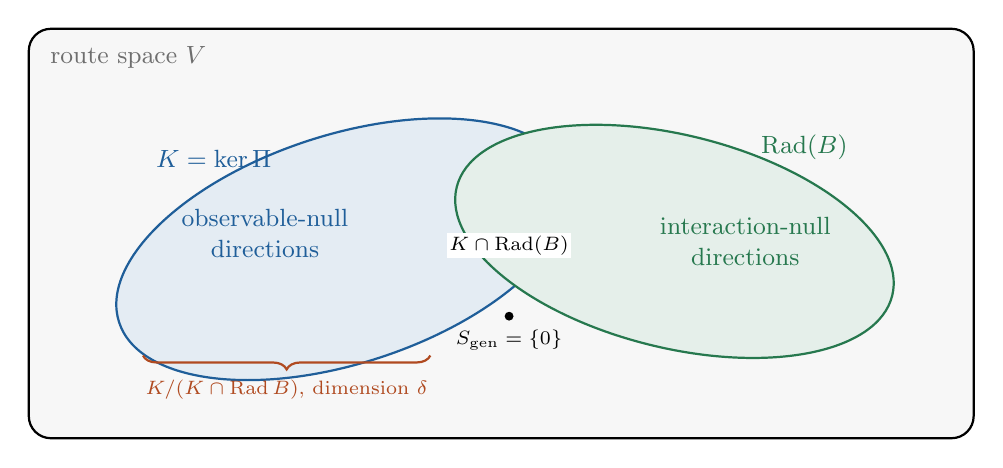
\begin{tikzpicture}[x=1cm,y=1cm,>=Stealth,font=\small]
 % ambient space
 \draw[rounded corners=8pt,thick,fill=gray!6] (0,0) rectangle (12,5.2);
 \node[anchor=north west,cGrey] at (0.15,5.1) {route space $V$};
 % K
 \draw[cObs,thick,fill=cObs!12,rotate around={18:(4.0,2.4)}] (4.0,2.4) ellipse (3.0 and 1.45);
 \node[cObs] at (2.35,3.55) {$K=\ker\Pi$};
 \node[cObs,align=center] at (3.0,2.6) {observable-null\\directions};
 % Rad
 \draw[cRel,thick,fill=cRel!12,rotate around={-14:(8.2,2.5)}] (8.2,2.5) ellipse (2.85 and 1.35);
 \node[cRel] at (9.85,3.7) {$\Rad(B)$};
 \node[cRel,align=center] at (9.1,2.5) {interaction-null\\directions};
 % overlap region label
 \node[font=\scriptsize,align=center,fill=white,inner sep=1pt] at (6.1,2.45) {$K\cap\Rad(B)$};
 % zero
 \fill (6.1,1.55) circle (1.6pt); \node[font=\scriptsize,below] at (6.1,1.5) {$S_{\mathrm{gen}}=\{0\}$};
 % deficit brace
 \draw[decorate,decoration={brace,amplitude=5pt,mirror},cHid,thick] (1.45,1.05) -- (5.1,1.05)
   node[midway,below=5pt,align=center,font=\scriptsize] {$K/(K\cap\Rad B)$,\ dimension $\defic$};
\end{tikzpicture}
\caption{The three equivalences as three subspaces. Observable equivalence implies interaction equivalence exactly when the left ellipse lies inside the right one. The part of $K$ that sticks out of $\Rad(B)$ is the relational content invisible to $\Pi$; its dimension is the relational deficit $\defic$ (Prop.~\ref{prop:deficit}).}\label{fig:equiv}
\end{figure}

%=====================================================================
\section{Interaction Preservation}\label{sec:interaction}
%=====================================================================
This section answers: for which observation maps $\Pi$ does a bilinear pairing $B$ \emph{descend}, that is, satisfy $B(X,Y)=\bar B(\Pi X,\Pi Y)$ for a bilinear $\bar B$ on $O$?

\subsection{The Observable Quotient Criterion}
\begin{theorem}[Observable Quotient Criterion --- Result I]\label{thm:quot}
Let $\Pi\colon V\to O$ be linear and onto with kernel $K$, and let $B\colon V\times V\to\RR$ be bilinear. The following are equivalent.
\begin{enumerate}[label=(\alph*)]
\item There is a bilinear $\bar B\colon O\times O\to\RR$ with $B(X,Y)=\bar B(\Pi X,\Pi Y)$ for all $X,Y$.
\item $\Pi X=\Pi X'$ and $\Pi Y=\Pi Y'$ imply $B(X,Y)=B(X',Y')$.
\item $K\subseteq\Rad_L(B)\cap\Rad_R(B)$.
\end{enumerate}
When they hold, $\bar B$ is unique. No finiteness, symmetry or field-specific hypothesis beyond linearity is used.
\end{theorem}
\begin{proof}
(a)$\Rightarrow$(b) is immediate. (b)$\Rightarrow$(c): let $k\in K$. Then $\Pi k=\Pi 0$, so for every $Y$, $B(k,Y)=B(0,Y)=0$; hence $k\in\Rad_L$; symmetrically $k\in\Rad_R$.
(c)$\Rightarrow$(a): for fixed $Y$ the linear functional $B(\cdot,Y)$ vanishes on $K$, so by Lemma~\ref{lem:universal} there is a unique linear functional $\beta_Y$ on $O$ with $B(X,Y)=\beta_Y(\Pi X)$. For fixed $o\in O$ pick $X$ with $\Pi X=o$; then $Y\mapsto\beta_Y(o)=B(X,Y)$ is linear and vanishes on $K$ because $K\subseteq\Rad_R$; so it factors through $\Pi$ as $\Pi Y\mapsto\bar B(o,\Pi Y)$. Linearity of $\bar B$ in $o$ follows from that of $B$ in $X$. Uniqueness: $\Pi$ is onto.
\end{proof}
\status{standard (universal property of quotients applied to bilinear maps~\cite{Lan02,Rom08,Mac71}); stated and proved here in the generality used below.}

\begin{corollary}\label{cor:sym}
If $B$ is symmetric or antisymmetric, $B$ descends to $\Pi$ iff $K\subseteq\Rad(B)$, i.e.\ iff the single condition $B(k,\cdot)=0$ holds for all observable-null $k$.
\end{corollary}

\begin{proposition}[One-sided descent]\label{prop:onesided}
$B(X,Y)=\tilde B(\Pi X,Y)$ for a bilinear $\tilde B\colon O\times V\to\RR$ iff $K\subseteq\Rad_L(B)$; analogously for the second slot with $\Rad_R(B)$.
\end{proposition}
\begin{proof}
Lemma~\ref{lem:universal} applied to $X\mapsto B(X,Y)$ for each $Y$.
\end{proof}
Proposition~\ref{prop:onesided} shows that \emph{both} radicals are needed in Theorem~\ref{thm:quot}:

\begin{example}[One-sided descent only]\label{ex:onesided}
$V=\RR^2$, $\Pi(x,y)=x$, $B(X,Y)=x\,y'$. Then $K=\spn\{(0,1)\}$, $B(k,\cdot)=0$ for $k\in K$ so $K\subseteq\Rad_L$, but $B(\cdot,k)=x\neq0$ so $K\not\subseteq\Rad_R$. $B$ depends on its first argument only through $\Pi$, but on the second through $y'$; it does not descend.
\end{example}

\subsection{Resolution ordering}
\begin{proposition}[Interaction quotient and resolution]\label{prop:resolution}
Let $q_L\colon V\to V/\Rad_L(B)$ and $q_R\colon V\to V/\Rad_R(B)$. Then $B$ factors canonically as $B=\hat B(q_L\cdot,q_R\cdot)$ with $\hat B$ nondegenerate, and
\[ B\text{ descends to }\Pi\iff q_L\text{ and }q_R\text{ both factor through }\Pi. \]
\end{proposition}
\begin{proof}
Nondegeneracy of $\hat B$ is the definition of the radicals. $q_L$ factors through $\Pi$ iff $K\subseteq\ker q_L=\Rad_L$ (Lemma~\ref{lem:universal}); likewise for $q_R$. Apply Theorem~\ref{thm:quot}.
\end{proof}
In words: \emph{the observable resolution must dominate the interaction resolution}. If $\Pi$ is coarser than $q_L$ or $q_R$ in the quotient-refinement order, some interaction information is invisible to $\Pi$.

\subsection{Relational deficit}
\begin{definition}[Relational deficit]\label{def:deficit}
$\defic(\Pi,B):=\dim\bigl(K/(K\cap\Rad(B))\bigr)\in\{0,1,2,\dots\}\cup\{\infty\}$ (cardinal dimension in general).
For finite-dimensional data define also the left and right obstruction ranks
$\rho_L=\dim K/(K\cap\Rad_L(B))=\rk\bigl(X\mapsto B(X,\cdot)\big|_K\bigr)$ and $\rho_R$ analogously.
\end{definition}

\begin{proposition}[Properties of the deficit]\label{prop:deficit}
\begin{enumerate}[label=(\roman*)]
\item $\defic=0$ iff $B$ descends to $\Pi$.
\item $\max(\rho_L,\rho_R)\le\defic\le\rho_L+\rho_R$; if $B$ is symmetric or antisymmetric, $\defic=\rho_L=\rho_R$.
\item (Matrix formula.) In bases, let the columns of $\mathsf K$ span $\ker\Pi$ and let $\mathsf B_{ij}=B(e_i,e_j)$. Then
\[ \defic=\rk\begin{pmatrix}\mathsf B\mathsf K\\ \mathsf B^{\!\top}\mathsf K\end{pmatrix},\qquad \rho_L=\rk(\mathsf B^{\!\top}\mathsf K),\qquad\rho_R=\rk(\mathsf B\mathsf K). \]
\item (Minimal completion.) Let $\Psi\colon V\to W$ be linear. $B$ descends to $(\Pi,\Psi)\colon V\to O\oplus W$ iff $K\cap\ker\Psi\subseteq\Rad(B)$. If $\defic<\infty$, the least $\dim W$ for which such a $\Psi$ exists equals $\defic$.
\end{enumerate}
\end{proposition}
\begin{proof}
(i) is Theorem~\ref{thm:quot} in the form $K\subseteq\Rad(B)$.
(ii) Since $K\cap\Rad\subseteq K\cap\Rad_L$, $\rho_L\le\defic$; likewise $\rho_R\le\defic$. The map $K/(K\cap\Rad)\to K/(K\cap\Rad_L)\oplus K/(K\cap\Rad_R)$, $k\mapsto([k],[k])$ is injective, giving $\defic\le\rho_L+\rho_R$. For symmetric/antisymmetric $B$ all radicals coincide.
(iii) Write $k=\mathsf Kc$. Then $k\in\Rad_L$ iff $k^{\!\top}\mathsf B=0$ iff $\mathsf B^{\!\top}\mathsf Kc=0$, and $k\in\Rad_R$ iff $\mathsf B\mathsf Kc=0$. So $K\cap\Rad(B)$ corresponds to the null space of the stacked matrix and $\defic=\dim K-\dim\ker=\rk$.
(iv) The kernel of $(\Pi,\Psi)$ is $K\cap\ker\Psi$; apply Theorem~\ref{thm:quot}. If $K\cap\ker\Psi\subseteq\Rad(B)$ then $\Psi|_K$ has kernel inside $K\cap\Rad$, so $\dim W\ge\dim K/(K\cap\Rad)=\defic$. Conversely let $\Psi_0\colon K\to K/(K\cap\Rad)$ be the quotient map and extend it linearly to $V$ (choose a complement of $K$); then $K\cap\ker\Psi=K\cap\Rad$ and $\dim W=\defic$.
\end{proof}
\status{elementary; the deficit and the minimal-completion statement are formulations introduced here. Verified numerically on 300 random instances (Appendix~\ref{app:tests}).}

Informally, $\defic$ counts the independent pieces of generative structure that are invisible to the observable representation yet visible to the interaction. In the example of \S\ref{sec:smallest}, $K=\spn\{(0,1)\}$, $\Rad(B)=0$, hence $\defic=1$: one extra observable ($y$) is exactly what is needed.

\subsection{Self-interaction and representatives}\label{sec:represent}
Two further statements explain why the obstruction cannot be detected from the wrong data, and why the pairing induced on observables is not canonical.

\begin{proposition}[Self-interaction]\label{prop:self}
Let $B$ be symmetric and $Q(X)=B(X,X)$. Then $Q(X)=\bar Q(\Pi X)$ for some function $\bar Q$ on $O$ iff $B$ descends to $\Pi$.
\end{proposition}
\begin{proof}
If $B$ descends, $Q(X)=\bar B(\Pi X,\Pi X)$. Conversely let $k\in K$, $X\in V$, $t\in\RR$. Then $0=Q(X+tk)-Q(X)=2tB(X,k)+t^2B(k,k)$ for all $t$, so $B(X,k)=0$ for all $X$ and $B(k,k)=0$. Hence $K\subseteq\Rad_R(B)=\Rad(B)$ by symmetry.
\end{proof}
The self-interaction is a function of the observable \emph{only} if it is constant on every fibre $X+K$. A refinement $T$ with $B(TX,TX)=B(X,X)$ (a consequence of joint invariance) tests constancy on the two-point set $\{X,TX\}\subseteq X+K$ only. In the hidden-sector model of \S\ref{sec:modelH}, $Q(X+k)-Q(X)=-\tfrac12h_k\!\cdot h_k-h_k\!\cdot h_X$, which vanishes at $k=-2h_X$ (the refinement partner, where $h_{X+k}=-h_X$) but not for general $k\in K$. Joint invariance is therefore the wrong test for observable adequacy.

\begin{proposition}[Representatives]\label{prop:sections}
Let $\sigma\colon O\to V$ be a linear section of $\Pi$ ($\Pi\sigma=\id_O$) and put $B_\sigma(o,o')=B(\sigma o,\sigma o')$.
\begin{enumerate}[label=(\alph*)]
\item Every other linear section is $\sigma'=\sigma+\kappa$ with $\kappa\colon O\to K$ linear, and
\[ B_{\sigma'}(o,o')-B_\sigma(o,o')=B(\sigma o,\kappa o')+B(\kappa o,\sigma o')+B(\kappa o,\kappa o'). \]
\item If $B$ descends, $B_\sigma=\bar B$ for every $\sigma$.
\item If $B$ is symmetric, $O\ne0$, and $B_\sigma$ does not depend on $\sigma$, then $B$ descends.
\end{enumerate}
In the hidden-sector model, the linear sections are $\sigma_H(s)=(s,Hs)$ in $(s,h)$-coordinates with $H\in\RR^{3\times3}$ arbitrary, and
\[ B_{\sigma_H}(s,s')=-\tfrac12\,s^{\!\top}(\mathsf I+H^{\!\top}H)\,s'. \]
\end{proposition}
\begin{proof}
(a) $\kappa=\sigma'-\sigma$ lands in $K$ because $\Pi\sigma'=\Pi\sigma$; the formula is bilinearity. (b) is Theorem~\ref{thm:quot}. (c) The hypothesis $O\ne0$ is needed: for $V=\RR$, $O=0$, $B(x,y)=xy$ the only section is $0$, so $B_\sigma$ is trivially independent of $\sigma$, yet $K=V$ and $\Rad(B)=0$. Now let $k\in K$, $0\ne\varphi\in O^*$ (which exists since $O\ne0$), and apply (a) with $\kappa=t\,\varphi(\cdot)k$. The coefficient of $t^2$ is $\varphi(o)\varphi(o')B(k,k)$, forcing $B(k,k)=0$. The coefficient of $t$ is $\varphi(o')B(\sigma o,k)+\varphi(o)B(\sigma o',k)$ (using symmetry); taking $o=o'$ with $\varphi(o)\neq0$ gives $B(\sigma o,k)=0$ on a set that spans $O$, hence for all $o$. Finally every $X\in V$ is $X=\sigma\Pi X+k'$ with $k'\in K$, and polarising $B(k,k)=0$ on the subspace $K$ gives $B(K,K)=0$; so $B(X,k)=0$ for all $X$ and $K\subseteq\Rad(B)$. The displayed formula is the model-$H$ pairing evaluated on $\sigma_H(s)=(s,Hs)$.
\end{proof}
\status{elementary. The model-$H$ formula is reproduced numerically (Appendix~\ref{app:tests}).}
Thus the pairing one would \emph{read off} on observables by choosing a representative of each observable value is canonical exactly when the interaction descends. In the hidden-sector model every choice of $H$ gives a legitimate but different observable pairing, from $-\tfrac12s\!\cdot s'$ at $H=0$ to arbitrarily large magnitudes; the observation map alone does not select among them.

%=====================================================================
\section{The Quotient Obstruction}\label{sec:obstruction}
%=====================================================================
We now give three families in which the obstruction is present although every ``natural'' symmetry is respected.

\subsection{The hidden-sector model}\label{sec:modelH}
Let $V=\RR^3\oplus\RR^3$ with elements $X=(u,v)$. Define the observable and internal components
\[ s=u+v,\qquad h=u-v, \]
the observation map $\Pi(X)=s_X\in\RR^3$, the pairing
\begin{equation}\label{eq:BH}
B(X,Y)=-\tfrac12\bigl(s_X\!\cdot s_Y+h_X\!\cdot h_Y\bigr),
\end{equation}
and the refinement $T(u,v)=(v,u)$, which in the new coordinates reads
\begin{equation}\label{eq:Th}
T(s,h)=(s,-h).
\end{equation}
\begin{proposition}[Properties of the hidden-sector model]\label{prop:H}
\begin{enumerate}[label=(\alph*)]
\item $B(X,Y)=-(u_X\!\cdot u_Y+v_X\!\cdot v_Y)$; $B$ is symmetric, negative definite, $\Rad(B)=0$.
\item $\Pi T=\Pi$, $h_{TX}=-h_X$ (observable component unchanged, internal component reversed).
\item Joint invariance: $B(TX,TY)=B(X,Y)$.
\item $B(TX,Y)=B(X,Y)+h_X\!\cdot h_Y$; hence independent invariance fails.
\item $K=\{(u,-u)\}=\{s=0\}$, $\dim K=3$, and $\spn\{X-TX\}=K$.
\item $\defic(\Pi,B)=3$. In particular $B$ does \emph{not} descend to $\Pi$: for $k=(u,-u)$ and every $Y$, $B(k,Y)=-\tfrac12h_k\!\cdot h_Y=-u\!\cdot h_Y$.
\end{enumerate}
\end{proposition}
\begin{proof}
(a) $s\!\cdot\!s'+h\!\cdot\!h'=(u{+}v)\!\cdot\!(u'{+}v')+(u{-}v)\!\cdot\!(u'{-}v')=2(u\!\cdot\!u'+v\!\cdot\!v')$.
(b) $s_{TX}=v+u=s_X$, $h_{TX}=v-u=-h_X$.
(c) $B(TX,TY)=-\tfrac12(s_X\!\cdot s_Y+(-h_X)\!\cdot(-h_Y))$.
(d) $B(TX,Y)=-\tfrac12(s_X\!\cdot s_Y-h_X\!\cdot h_Y)=B(X,Y)+h_X\!\cdot h_Y$.
(e) $s=0\iff v=-u$. $X-TX=(u-v,v-u)\in K$ and every $(w,-w)$ arises with $u=w/2$, $v=-w/2$.
(f) $K\cap\Rad(B)=0$ as $\Rad(B)=0$, so $\defic=\dim K=3$; the displayed value of $B(k,Y)$ follows from~\eqref{eq:BH} with $s_k=0$, $h_k=2u$.
\end{proof}
\begin{example}[Concrete witness]\label{ex:witness}
Let $\mathbf e_x=(1,0,0)$ and take $X=(\mathbf e_x,\mathbf 0)$, $X'=TX=(\mathbf 0,\mathbf e_x)$. Then $\Pi X=\Pi X'=\mathbf e_x$, but with $Y=X$: $B(X,X)=-1$ and $B(X',X)=0$.
Moreover $B(X,X)=B(X',X')=-1$, so the two routes agree on observable value and on self-interaction, and differ in their mutual interaction with $X$.
\end{example}
This is exactly the structure of the minimal example of \S\ref{sec:smallest}, with a three-dimensional hidden sector.

\subsection{The Legendre family on the route space of directions}\label{sec:legendre}
Let $V=F(S^2)$ with $\Pi(r(\mathbf a))=\mathbf a\in\RR^3$ (Example~\ref{ex:free}), and let $P_\ell$ be the Legendre polynomial of degree $\ell$. For $\ell\ge1$ define $B_\ell$ on generators by
\begin{equation}\label{eq:Bell}
B_\ell\bigl(r(\mathbf a),r(\mathbf b)\bigr)=-P_\ell(\mathbf a\cdot\mathbf b),
\end{equation}
extended bilinearly. In particular $B_1(r(\mathbf a),r(\mathbf b))=-\mathbf a\cdot\mathbf b$ and $B_3=-P_3(\mathbf a\cdot\mathbf b)$ with $P_3(x)=\tfrac12(5x^3-3x)$.

\begin{theorem}[The Legendre family]\label{thm:legendre}
\begin{enumerate}[label=(\roman*)]
\item (Admissibility profile.) $B_\ell$ is symmetric, satisfies $B_\ell(r(\mathbf a),r(\mathbf a))=-1$, and $-B_\ell$ is positive semidefinite on $V$; it is covariant under rotations,
\[ B_\ell\bigl(r(R\mathbf a),r(R\mathbf b)\bigr)=B_\ell\bigl(r(\mathbf a),r(\mathbf b)\bigr),\qquad R\in O(3), \]
and, for odd $\ell$, $B_\ell(r(-\mathbf a),r(\mathbf b))=-B_\ell(r(\mathbf a),r(\mathbf b))$.
\item $B_1$ descends to $\Pi$: $B_1(X,Y)=-\Pi X\cdot\Pi Y$; $\defic(\Pi,B_1)=0$.
\item For every $\ell\ge2$, $B_\ell$ does not descend to $\Pi$, and $\defic(\Pi,B_\ell)=\rho_L=\rho_R=2\ell+1$.
\end{enumerate}
\end{theorem}
\begin{proof}
(i) Rotation invariance of $\mathbf a\cdot\mathbf b$; $P_\ell(1)=1$; $P_\ell(-x)=(-1)^\ell P_\ell(x)$. Let $S_{\ell m}$, $m=1,\dots,2\ell+1$, be real orthonormal spherical harmonics of degree $\ell$. The addition theorem~\cite{AAR99} gives
\begin{equation}\label{eq:addition}
P_\ell(\mathbf a\cdot\mathbf b)=\frac{4\pi}{2\ell+1}\sum_{m=1}^{2\ell+1}S_{\ell m}(\mathbf a)S_{\ell m}(\mathbf b).
\end{equation}
Define linear functionals $f_m\colon V\to\RR$ by $f_m(r(\mathbf a))=S_{\ell m}(\mathbf a)$. Then
\begin{equation}\label{eq:Bf}
B_\ell(X,Y)=-c_\ell\sum_m f_m(X)f_m(Y),\qquad c_\ell=\tfrac{4\pi}{2\ell+1}>0,
\end{equation}
so $-B_\ell(X,X)=c_\ell\sum f_m(X)^2\ge0$.
(ii) $P_1(x)=x$ and $B_1(r(\mathbf a),r(\mathbf b))=-\Pi r(\mathbf a)\cdot\Pi r(\mathbf b)$; both sides are bilinear and agree on generators.
(iii) The $f_m$ are linearly independent functionals on $V$ because the $S_{\ell m}$ are linearly independent functions on $S^2$ (evaluate on generators). Consequently $F=(f_1,\dots,f_{2\ell+1})\colon V\to\RR^{2\ell+1}$ is onto, and by~\eqref{eq:Bf}, $B_\ell(X,\cdot)=0\iff\sum_mf_m(X)f_m=0\iff F(X)=0$; so $\Rad(B_\ell)=\ker F$ and
\[ \defic=\dim K/(K\cap\ker F)=\dim F(K). \]
Suppose $F(K)\neq\RR^{2\ell+1}$. Then there is $c\neq0$ with $c\cdot F(X)=0$ for all $X\in K$, i.e.\ the functional $\varphi=\sum c_mf_m$ vanishes on $K=\ker\Pi$. By Lemma~\ref{lem:universal}, $\varphi=w\circ\Pi$ for some $w\in\RR^3$. Evaluating on generators, $\sum_mc_mS_{\ell m}(\mathbf a)=w\cdot\mathbf a$ for all $\mathbf a\in S^2$. The left side is a spherical harmonic of degree $\ell$, the right a harmonic of degree $1$; for $\ell\neq1$ these are orthogonal in $L^2(S^2)$, so both vanish, and $c=0$ by independence: contradiction. Hence $F(K)=\RR^{2\ell+1}$ and $\defic=2\ell+1$. Symmetry of $B_\ell$ gives $\rho_L=\rho_R=\defic$ (Prop.~\ref{prop:deficit}(ii)).
\end{proof}

\begin{example}[Explicit witness, $\ell=3$]\label{ex:P3}
Let $\mathbf n=\tfrac12\mathbf e_x+\tfrac{\sqrt3}2\mathbf e_y$ and
\[ X=r(\mathbf n)-\tfrac12\,r(\mathbf e_x)-\tfrac{\sqrt3}2\,r(\mathbf e_y). \]
Then $\Pi X=\mathbf n-\tfrac12\mathbf e_x-\tfrac{\sqrt3}2\mathbf e_y=0$, so $X\in K$. Using $P_3(\tfrac12)=-\tfrac7{16}$, $P_3(1)=1$, $P_3(0)=0$:
\[ B_1\bigl(X,r(\mathbf e_x)\bigr)=-\tfrac12+\tfrac12=0,\qquad
 B_3\bigl(X,r(\mathbf e_x)\bigr)=\tfrac7{16}+\tfrac12=\tfrac{15}{16}. \]
Hence $X\notin\Rad_L(B_3)$ although $\Pi X=0$. The same $X$ gives, for $\ell=5$ ($P_5(\tfrac12)=\tfrac{23}{256}$), $B_5(X,r(\mathbf e_x))=\tfrac{105}{256}$.
\end{example}

\begin{example}[A four-route table]\label{ex:four}
Restrict to the four elementary routes $r_1=r(\mathbf e_x)$, $r_2=r(\mathbf e_y)$, $r_3=r(\mathbf e_z)$, $r_4=r(\mathbf n)$, with $\mathbf n=(\tfrac12,\tfrac{\sqrt3}2,0)$. Then the route space is $V_4=\RR^4$, $\Pi$ has matrix $(\mathbf e_x\ \mathbf e_y\ \mathbf e_z\ \mathbf n)$, $K=\spn\{k\}$ with $k=(-\tfrac12,-\tfrac{\sqrt3}2,0,1)^{\!\top}$, and the Gram matrices of $B_1$ and $B_3$ are
\[
G_1=-\begin{pmatrix}1&0&0&\tfrac12\\0&1&0&\tfrac{\sqrt3}2\\0&0&1&0\\\tfrac12&\tfrac{\sqrt3}2&0&1\end{pmatrix},\qquad
G_3=\begin{pmatrix}-1&0&0&\tfrac7{16}\\0&-1&0&-\tfrac{3\sqrt3}{16}\\0&0&-1&0\\\tfrac7{16}&-\tfrac{3\sqrt3}{16}&0&-1\end{pmatrix},
\]
using $P_3(\tfrac{\sqrt3}2)=\tfrac{3\sqrt3}{16}$. Then
\[ G_1k=0,\qquad G_3k=\Bigl(\tfrac{15}{16},\ \tfrac{5\sqrt3}{16},\ 0,\ -\tfrac{15}{16}\Bigr)^{\!\top}\neq0, \]
so $\defic=0$ for $B_1$ and $\defic=1$ for $B_3$ on this four-route space: the single observable-null route $k$ interacts nontrivially with $r_1$, $r_2$ and $r_4$ under $B_3$ and with nothing under $B_1$. Every entry is verified in exact arithmetic over $\mathbb Q(\sqrt3)$ (Appendix~\ref{app:tests}).
\end{example}

\begin{table}[t]
\centering\small
\renewcommand{\arraystretch}{1.55}
\begin{tabular}{@{}lccc@{}}
\toprule
 & $\ell=1$ & $\ell=3$ & $\ell=5$\\
\midrule
$C=B_\ell(r(\mathbf a),r(\mathbf b))$ at $60^\circ$ ($\mathbf a\!\cdot\!\mathbf b=\dfrac12$) & $-\dfrac12$ & $+\dfrac7{16}$ & $-\dfrac{23}{256}$\\
$\dfrac14(1+C)$ & $\dfrac18=0.125$ & $\dfrac{23}{64}=0.359375$ & $\dfrac{233}{1024}$\\
$B_\ell(X,r(\mathbf e_x))$ for the $X\in K$ of Ex.~\ref{ex:P3} & $0$ & $\dfrac{15}{16}$ & $\dfrac{105}{256}$\\
$\defic(\Pi,B_\ell)$ & $0$ & $7$ & $11$\\
\bottomrule
\end{tabular}
\caption{Values (exact fractions, reproduced by the verification script of \S\ref{sec:repro}). The second row applies the binary joint-event representation $P(A,B\mid\mathbf a,\mathbf b)=\tfrac14(1+AB\,C)$ proved in GCT v002~\cite{G2} purely as arithmetic on the first row; no probabilistic claim is made in this paper.}\label{tab:legendre}
\end{table}

\begin{remark}[Antipodal quotient]
If one prefers a route space in which $r(-\mathbf a)=-r(\mathbf a)$, replace $F(S^2)$ by its quotient by $\spn\{r(\mathbf a)+r(-\mathbf a)\}$. For odd $\ell$, $\Pi$ and $B_\ell$ are well defined on the quotient, the witness of Example~\ref{ex:P3} lives there unchanged, and the proof of Theorem~\ref{thm:legendre}(iii) goes through verbatim because $S_{\ell m}$ are odd for odd $\ell$. The obstruction is therefore not an artefact of freeness.
\end{remark}

\begin{remark}[Relation to the GCT v002 underdetermination theorem]\label{rem:gct}
The v002 lock freezes the conditions $C(\mathbf a,\mathbf b)=c(a-b)$, $c(-d)=c(d)$, $c(0)=-1$, $c(d+\pi)=-c(d)$ together with $|c|\le1$~\cite{G8,G2}. For planar directions the kernels $c_\ell(d)=-P_\ell(\cos d)$, $\ell$ odd, satisfy all of them (checked in Appendix~\ref{app:tests} for $\ell=3$). In route-space language, \emph{what distinguishes $B_1$ from $B_3$ among these admissible pairings is precisely whether the pairing descends to the observable vector}: $\defic=0$ versus $\defic=7$. The descent condition $K\subseteq\Rad(B)$ is therefore a \emph{selection criterion} within the admissible class. It is not a derivation: whether UNNS recursion supplies it independently is open (\S\ref{sec:discussion}).
\end{remark}

\subsection{Illustration: many routes, one observable}
\begin{figure}[t]
\centering
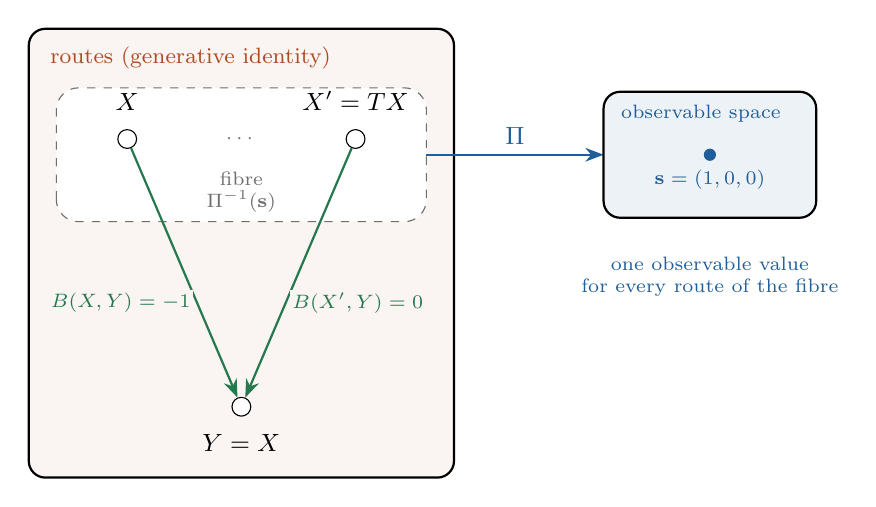
\begin{tikzpicture}[x=1cm,y=1cm,>=Stealth,font=\small]
 % route space
 \draw[rounded corners=6pt,thick,fill=cHid!6] (0,0) rectangle (5.4,5.7);
 \node[cHid,anchor=north west,font=\footnotesize] at (0.15,5.6) {routes (generative identity)};
 \draw[dashed,cGrey,rounded corners=8pt,fill=white] (0.35,3.25) rectangle (5.05,4.95);
 \node[cGrey,font=\scriptsize,align=center] at (2.7,3.62) {fibre\\$\Pi^{-1}(\mathbf s)$};
 \node[draw,circle,fill=white,inner sep=2.4pt] (x1) at (1.25,4.3) {};
 \node[draw,circle,fill=white,inner sep=2.4pt] (x2) at (4.15,4.3) {};
 \node[font=\scriptsize,cGrey] at (2.7,4.3) {$\cdots$};
 \node[above=3pt of x1] {$X$}; \node[above=3pt of x2] {$X'=TX$};
 \node[draw,circle,fill=white,inner sep=2.4pt] (y) at (2.7,0.9) {};
 \node[below=3pt of y] {$Y=X$};
 \draw[->,thick,cRel] (x1) -- (y) node[pos=0.62,left=1pt,font=\scriptsize,cRel,fill=cHid!6,inner sep=1pt] {$B(X,Y)=-1$};
 \draw[->,thick,cRel] (x2) -- (y) node[pos=0.62,right=1pt,font=\scriptsize,cRel,fill=cHid!6,inner sep=1pt] {$B(X',Y)=0$};
 % observation
 \draw[->,thick,cObs] (5.05,4.1) -- (7.3,4.1) node[midway,above] {$\Pi$};
 \draw[rounded corners=6pt,thick,fill=cObs!8] (7.3,3.3) rectangle (10.0,4.9);
 \node[cObs,anchor=north west,font=\scriptsize] at (7.4,4.85) {observable space};
 \fill[cObs] (8.65,4.1) circle (2.2pt);
 \node[cObs,font=\scriptsize,below=2pt] at (8.65,4.1) {$\mathbf s=(1,0,0)$};
 \node[cObs,font=\scriptsize,align=center] at (8.65,2.55) {one observable value\\for every route of the fibre};
\end{tikzpicture}
\caption{Many routes, one observable. The hidden-sector model of \S\ref{sec:modelH} (Example~\ref{ex:witness}): $X$ and $X'=TX$ lie in one fibre of $\Pi$ and have the same self-interaction $B(X,X)=B(X',X')=-1$, but different pairings with $Y=X$.}\label{fig:many}
\end{figure}

%=====================================================================
\section{Refinement and Relational Invariance}\label{sec:refinement}
%=====================================================================
The hidden-sector model of \S\ref{sec:modelH} has a refinement $T$ for which the interaction is invariant under the simultaneous refinement of both arguments. This section isolates what that does and does not imply.

\subsection{Joint refinement invariance does not eliminate hidden interactions}\label{sec:joint}
\begin{theorem}[Result II]\label{thm:joint}
There exist a linear route system $(V,\Pi,B,\{T\})$ with $\Pi T=\Pi$, $\spn\{X-TX\}=\ker\Pi$, and $B$ symmetric, nondegenerate and jointly invariant, $B(TX,TY)=B(X,Y)$, such that $B$ does not descend to $\Pi$ and $\defic(\Pi,B)=\dim\ker\Pi>0$.
\end{theorem}
\begin{proof}
The hidden-sector model, Proposition~\ref{prop:H}(b)--(f).
\end{proof}
Thus joint refinement invariance need not eliminate interactions involving individually unobserved structural distinctions: $B(TX,Y)-B(X,Y)=h_X\!\cdot h_Y$ is nonzero whenever the internal components of $X$ and $Y$ overlap, even though the same distinction cancels when \emph{both} routes are refined.

\subsection{Involutive refinements: a block decomposition}\label{sec:invol}
\begin{proposition}[Involutive refinement]\label{prop:invol}
Let $T$ be a refinement ($\Pi T=\Pi$) with $T^2=\id$. Put $V_\pm=\{X:\ TX=\pm X\}$, so $V=V_+\oplus V_-$, and assume $\ker\Pi=V_-$ (so that $\Pi|_{V_+}$ is injective). Then:
\begin{enumerate}[label=(\alph*)]
\item $B$ is jointly invariant iff $B(V_+,V_-)=B(V_-,V_+)=0$, i.e.\ $B=B|_{V_+}\oplus B|_{V_-}$.
\item $B$ is left-invariant iff $V_-\subseteq\Rad_L(B)$; right-invariant iff $V_-\subseteq\Rad_R(B)$.
\item Under joint invariance, $B$ descends to $\Pi$ iff $B|_{V_-\times V_-}=0$. In that case $B=B|_{V_+}$ and $\defic=0$; in general $\defic=\dim V_-/\bigl(V_-\cap\Rad(B|_{V_-})\bigr)$.
\end{enumerate}
\end{proposition}
\begin{proof}
We use that the characteristic of $\RR$ is not $2$. (a) For $x\in V_+$, $y\in V_-$: joint invariance gives $B(x,y)=B(Tx,Ty)=-B(x,y)$, hence $B(x,y)=0$; similarly for $B(y,x)$. Conversely if $B$ is block diagonal, write $X=x_++x_-$, $Y=y_++y_-$ and compute $B(TX,TY)=B(x_+,y_+)+B(x_-,y_-)=B(X,Y)$.
(b) $B(TX,Y)-B(X,Y)=-2B(x_-,Y)$.
(c) $K=V_-\subseteq\Rad(B)$ iff $B(V_-,V_-)=0$ in view of the block structure; the formula for $\defic$ follows because $B(V_-,V_+)=0$.
\end{proof}
The hidden-sector model is the case $V_+=\{h=0\}$, $V_-=\{s=0\}$ with $B|_{V_-}=-\tfrac12h\!\cdot h'$ nondegenerate. Joint invariance is exactly the statement that no interaction couples the observable and the internal sector; it says nothing about the internal sector's \emph{own} interaction, which survives all refinements of both arguments.

\subsection{Diagonal versus factorwise coinvariants}\label{sec:coinv}
Let a group $G$ act on $V$ by refinements (so $\Pi g=\Pi$ for all $g\in G$) and write $V_G=V/\spn\{X-gX\}$ for the coinvariants~\cite{Bro82}.
\begin{proposition}[Joint versus independent invariance]\label{prop:coinv}
\begin{enumerate}[label=(\alph*)]
\item Bilinear forms that are \emph{independently} invariant (left and right) under $G$ are exactly the bilinear forms on $V$ that factor through $V_G\times V_G$, i.e.\ $(V_G\otimes V_G)^*$.
\item Bilinear forms that are \emph{jointly} invariant under $G$ are exactly $((V\otimes V)_G)^*$, coinvariants for the diagonal action $g\mapsto g\otimes g$.
\item The natural surjection $(V\otimes V)_G\twoheadrightarrow V_G\otimes V_G$ has kernel $N$, and the gap between joint and independent invariance is the space of functionals on $(V\otimes V)_G$ that do not vanish on $N$.
\end{enumerate}
For $G=\mathbb Z_2=\{1,T\}$ acting on $V=V_+\oplus V_-$ (over $\RR$): $V_G=V_+$, $(V\otimes V)_G=V_+\otimes V_+\oplus V_-\otimes V_-$, so $N=V_-\otimes V_-$.
\end{proposition}
\begin{proof}
(a) Left- and right-invariance say $B$ vanishes on $\spn\{X-gX\}\times V$ and $V\times\spn\{X-gX\}$, i.e.\ $B$ factors through $V_G\times V_G$ (universal property for each slot, as in Theorem~\ref{thm:quot}).
(b) Joint invariance says that the linear functional $\tilde B$ on $V\otimes V$ vanishes on $X\otimes Y-gX\otimes gY$.
(c) The natural map $V\otimes V\to V_G\otimes V_G$ sends the span of $X\otimes Y-gX\otimes gY$ into the span of $\{X-gX\}\otimes V+V\otimes\{Y-gY\}$ because $X\otimes Y-gX\otimes gY=(X-gX)\otimes Y+gX\otimes(Y-gY)$; so it descends. For $\mathbb Z_2$: $T\otimes T$ acts by $+1$ on $V_\pm\otimes V_\pm$ and $-1$ on $V_+\otimes V_-$ and $V_-\otimes V_+$, whose coinvariants vanish in characteristic $\ne2$.
\end{proof}
For the hidden-sector model, $\dim N=\dim V_-\otimes V_-=9$, and the hidden interaction $-\tfrac12h\!\cdot h'$ is a functional on $(V\otimes V)_G$ that is supported on $N$, hence invisible to $V_G\otimes V_G$. This is the algebraic reason that the joint/independent distinction is real: \emph{the diagonal coinvariants are strictly larger than the tensor square of the single-argument coinvariants}.

\begin{figure}[t]
\centering
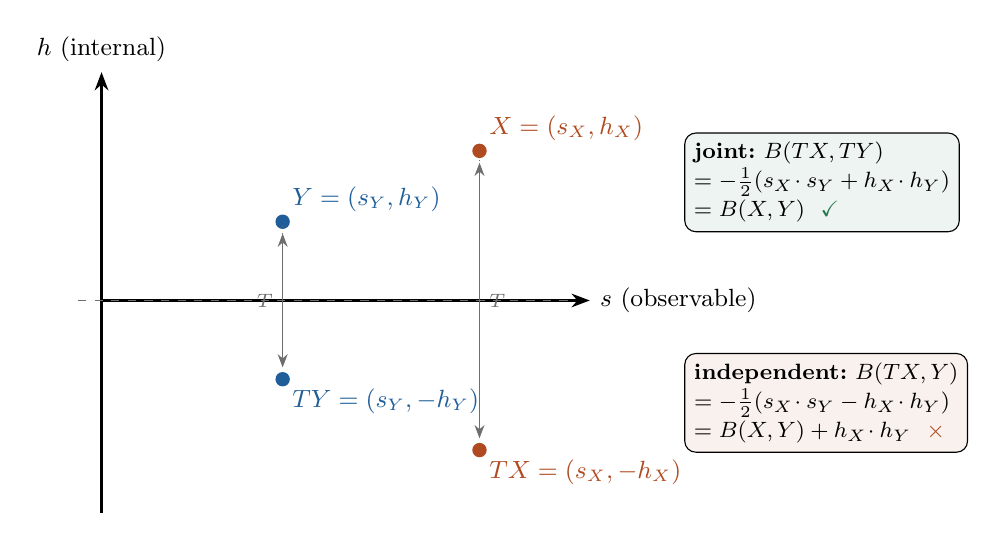
\begin{tikzpicture}[x=1cm,y=1cm,>=Stealth,font=\small]
 \draw[->,thick] (0,0) -- (6.2,0) node[right] {$s$ (observable)};
 \draw[->,thick] (0,-2.7) -- (0,2.9) node[above] {$h$ (internal)};
 \draw[dashed,cGrey] (-0.3,0) -- (6.0,0);
 % X, TX
 \fill[cHid] (4.8,1.9) circle (2.6pt) node[above right] {$X=(s_X,h_X)$};
 \fill[cHid] (4.8,-1.9) circle (2.6pt) node[below right] {$TX=(s_X,-h_X)$};
 % Y, TY
 \fill[cObs] (2.3,1.0) circle (2.6pt) node[above right] {$Y=(s_Y,h_Y)$};
 \fill[cObs] (2.3,-1.0) circle (2.6pt) node[below right] {$TY=(s_Y,-h_Y)$};
 \draw[<->,cGrey] (4.8,1.75) -- (4.8,-1.75) node[midway,right,font=\scriptsize] {$T$};
 \draw[<->,cGrey] (2.3,0.85) -- (2.3,-0.85) node[midway,left,font=\scriptsize] {$T$};
 \draw[dotted,cGrey] (4.8,0) -- (4.8,1.8); \draw[dotted,cGrey] (2.3,0) -- (2.3,1.0);
 % boxes
 \node[draw,rounded corners=4pt,fill=cRel!8,align=left,font=\footnotesize,anchor=west] at (7.4,1.5)
   {\textbf{joint:}\ $B(TX,TY)$\\[1pt]
    $=-\tfrac12(s_X\!\cdot s_Y+h_X\!\cdot h_Y)$\\[1pt]
    $=B(X,Y)$\ \ \textcolor{cRel}{$\checkmark$}};
 \node[draw,rounded corners=4pt,fill=cHid!8,align=left,font=\footnotesize,anchor=west] at (7.4,-1.3)
   {\textbf{independent:}\ $B(TX,Y)$\\[1pt]
    $=-\tfrac12(s_X\!\cdot s_Y-h_X\!\cdot h_Y)$\\[1pt]
    $=B(X,Y)+h_X\!\cdot h_Y$\ \ \textcolor{cHid}{$\times$}};
\end{tikzpicture}
\caption{Refinement and relational preservation (one scalar internal coordinate drawn). $T$ reflects the internal coordinate and fixes the observable one. Reflecting \emph{both} routes preserves the interaction; reflecting only one changes it by $h_X\!\cdot h_Y$.}\label{fig:refine}
\end{figure}

%=====================================================================
\section{The Observable-Null Compatibility Theorem}\label{sec:compat}
%=====================================================================

\subsection{Hypotheses}
Let $\{T_i\}_{i\in I}$ be a family of refinements of $(V,\Pi)$. We use two hypotheses.
\begin{description}[leftmargin=0pt,style=unboxed,itemsep=2pt]
\item[(H1) Observable preservation.] $\Pi T_i=\Pi$ for all $i$.
\item[(H2) Kernel generation.] $\ker\Pi=\spn\{X-T_iX:\ X\in V,\ i\in I\}$.
\end{description}
(H1) implies $\spn\{X-T_iX\}\subseteq\ker\Pi$; (H2) asserts that refinement differences exhaust the observable-null directions. Equivalently, $\Pi$ is (isomorphic to) the quotient of $V$ by the span of refinement differences: observable identity \emph{is} identity up to refinement.

\subsection{The theorem}
\begin{theorem}[Refinement-Compatibility Theorem --- Result III]\label{thm:compat}
Assume (H1) and (H2). Let $B$ be bilinear on $V$ satisfying independent invariance for every $i\in I$:
\[ B(T_iX,Y)=B(X,Y),\qquad B(X,T_iY)=B(X,Y)\qquad(X,Y\in V). \]
Then $\ker\Pi\subseteq\Rad_L(B)\cap\Rad_R(B)$; consequently $B$ factors through $\Pi$: $B(X,Y)=\bar B(\Pi X,\Pi Y)$ for a unique bilinear $\bar B$.
Conversely, (H1) alone shows that any $B$ which factors through $\Pi$ is independently invariant under every $T_i$. Hence, under (H1)--(H2),
\[ B\text{ independently invariant}\iff B\text{ factors through }\Pi\iff \ker\Pi\subseteq\Rad(B). \]
\end{theorem}
\begin{proof}
For each $X$ and $i$, left-invariance gives $B(X-T_iX,Y)=0$ for all $Y$, i.e.\ $X-T_iX\in\Rad_L(B)$; right-invariance gives $B(Y,X-T_iX)=0$, i.e.\ $X-T_iX\in\Rad_R(B)$. Radicals are subspaces, so by (H2) $\ker\Pi=\spn\{X-T_iX\}\subseteq\Rad_L\cap\Rad_R$. Apply Theorem~\ref{thm:quot}.
For the converse, if $B=\bar B(\Pi\cdot,\Pi\cdot)$ then $B(T_iX,Y)=\bar B(\Pi T_iX,\Pi Y)=\bar B(\Pi X,\Pi Y)=B(X,Y)$ by (H1), and likewise in the second slot.
\end{proof}
\status{elementary corollary of Theorem~\ref{thm:quot}, equivalently the universal property of the coinvariants $V_G\cong O$ applied to bilinear forms (Prop.~\ref{prop:coinv}(a)). What is new is the explicit separation of the hypotheses, below.}

\begin{corollary}[Hierarchy]\label{cor:hier}
Under (H1) the following implications hold and none can be reversed in general:
\begin{center}
independent invariance $\Longrightarrow$ joint invariance, \qquad factoring through $\Pi$ $\Longrightarrow$ independent invariance.
\end{center}
Under (H1)--(H2) additionally independent invariance $\Longrightarrow$ factoring through $\Pi$. Joint invariance $\not\Longrightarrow$ factoring, even under (H1)--(H2) (hidden-sector model).
\end{corollary}

\subsection{Sharpness of the hypotheses}\label{sec:sharp}
Each hypothesis of Theorem~\ref{thm:compat} is necessary in the following sense.
\begin{example}[Independent invariance without (H2)]\label{ex:noH2}
$V=\RR^2$, $\Pi(x,y)=x$, $\mathcal T=\{\id\}$, $B(X,Y)=yy'$. (H1) holds, $B$ is trivially independently invariant under $\id$, but $\spn\{X-X\}=0\subsetneq K=\spn\{(0,1)\}$, and $B$ does not descend ($\defic=1$). Refinements must be \emph{rich enough} to generate the observable-null directions.
\end{example}
\begin{example}[One-sided invariance]\label{ex:oneside}
$V=\RR^2$, $\Pi(x,y)=x$, $T(x,y)=(x,-y)$ (so (H1), (H2) hold) and $B(X,Y)=x\,y'$ (Example~\ref{ex:onesided}). $B$ is left-invariant, $B(TX,Y)=B(X,Y)$, but not right-invariant, and does not descend. \emph{Both} slots must be refined independently.
\end{example}
\begin{example}[Joint invariance only]
The hidden-sector model (Prop.~\ref{prop:H}) satisfies (H1), (H2), joint invariance and fails independent invariance and descent.
\end{example}

\begin{example}[Permutation refinements and a sum observable]\label{ex:perm}
Let $V=\RR^n$ ($n\ge2$), $\Pi(x)=\sum_ix_i\in\RR$, and let $\mathcal T=\{T_i\}$ be the adjacent transpositions $(i\ i{+}1)$, acting by permuting coordinates.
(H1) holds. $X-T_iX=(x_i-x_{i+1})(e_i-e_{i+1})$, so $\spn\{X-T_iX\}=\spn\{e_i-e_{i+1}\}=\{\sum x_i=0\}=\ker\Pi$: (H2) holds.
The space of bilinear forms invariant under all $T_i$ \emph{jointly} is two dimensional, spanned by $\langle x,y\rangle=\sum x_iy_i$ and $(\sum x_i)(\sum y_i)$; the space of \emph{independently} invariant forms is one dimensional, spanned by $(\sum x_i)(\sum y_i)$ --- exactly the forms that factor through $\Pi$, as Theorem~\ref{thm:compat} predicts. For $B=a\langle x,y\rangle+b(\sum x)(\sum y)$ with $a\ne0$, $K\cap\Rad(B)=0$ and $\defic=n-1$.
\end{example}
\begin{proof}[Verification]
Joint invariance under all transpositions makes $B$ an $S_n$-equivariant endomorphism of the permutation module $\RR^n=\mathbf 1\oplus\{\sum=0\}$, which has exactly two irreducible summands (non-isomorphic for $n\ge2$) --- a two-dimensional commutant. Independent invariance forces the $\{\sum=0\}$ block to vanish by Theorem~\ref{thm:compat} (equivalently, $B(e_i-e_{i+1},\cdot)=0$ for all $i$). The dimension counts are reproduced numerically for $n=5$ in Appendix~\ref{app:tests}.
\end{proof}
The example shows the theorem at work in a coarse-graining setting: a macroscopic sum is a complete observable for interactions that are invariant under \emph{each} micro-relabelling separately, and incomplete for interactions that are invariant only under simultaneous relabelling.

\subsection{The compatibility hierarchy}
Figure~\ref{fig:hier} summarises Theorem~\ref{thm:compat} and Corollary~\ref{cor:hier}, together with the examples that block each reverse arrow.
\begin{figure}[t]
\centering
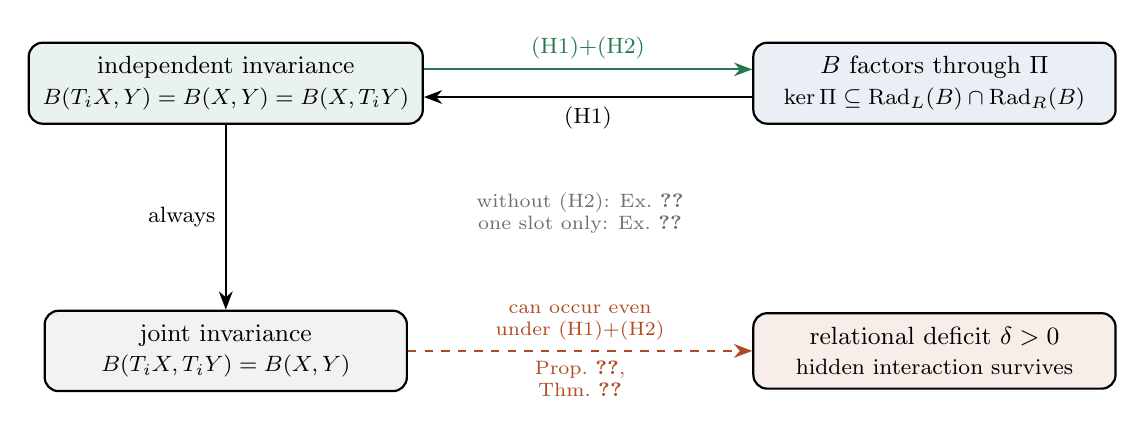
\begin{tikzpicture}[x=1cm,y=1cm,>=Stealth,font=\small,
  box/.style={draw,rounded corners=5pt,thick,align=center,inner sep=5pt,minimum width=4.6cm}]
 \node[box,fill=cRel!10] (sep) at (0,3.4) {independent invariance\\{\footnotesize $B(T_iX,Y)=B(X,Y)=B(X,T_iY)$}};
 \node[box,fill=cObs!10] (fac) at (9.0,3.4) {$B$ factors through $\Pi$\\{\footnotesize $\ker\Pi\subseteq\Rad_L(B)\cap\Rad_R(B)$}};
 \node[box,fill=gray!10] (joint) at (0,0) {joint invariance\\{\footnotesize $B(T_iX,T_iY)=B(X,Y)$}};
 \node[box,fill=cHid!10] (def) at (9.0,0) {relational deficit $\defic>0$\\{\footnotesize hidden interaction survives}};
 \draw[->,thick,cRel] ([yshift=5pt]sep.east) -- ([yshift=5pt]fac.west)
   node[midway,above,font=\footnotesize] {(H1)+(H2)};
 \draw[->,thick] ([yshift=-5pt]fac.west) -- ([yshift=-5pt]sep.east)
   node[midway,below,font=\footnotesize] {(H1)};
 \draw[->,thick] (sep) -- (joint) node[midway,left,font=\footnotesize] {always};
 \draw[->,thick,dashed,cHid] (joint) -- (def)
   node[midway,above,align=center,font=\scriptsize,cHid] {can occur even\\under (H1)+(H2)}
   node[midway,below,align=center,font=\scriptsize,cHid] {Prop.~\ref{prop:H},\\Thm.~\ref{thm:joint}};
 \node[font=\scriptsize,cGrey,align=center] at (4.5,1.75)
   {without (H2): Ex.~\ref{ex:noH2}\\one slot only: Ex.~\ref{ex:oneside}};
\end{tikzpicture}
\caption{The refinement-compatibility hierarchy. Independent invariance is the only refinement condition that reaches factorisation, and only together with (H1) and the kernel-generation hypothesis (H2). Joint invariance, however strong the symmetry, stops short: the converse of the left-hand vertical arrow fails.}\label{fig:hier}
\end{figure}

\subsection{Quantitative form}
\begin{proposition}\label{prop:quant}
Assume (H1)--(H2) with $V$ of finite dimension. For any bilinear $B$, $\defic(\Pi,B)=\dim\,q\bigl(\spn\{X-T_iX\}\bigr)$, where $q\colon V\to V/\Rad(B)$ is the quotient map; i.e.\ the deficit is the dimension of the image of the refinement differences in the interaction quotient. In particular $\defic=0$ iff $B$ is independently refinement invariant.
\end{proposition}
\begin{proof}
$\defic=\dim K/(K\cap\Rad)=\dim q(K)$, and $K=\spn\{X-T_iX\}$ by (H2). The last statement is Theorem~\ref{thm:compat}.
\end{proof}


%=====================================================================
\section{Generative Response Profiles}\label{sec:response}
%=====================================================================
Sections~\ref{sec:quot}--\ref{sec:compat} ask what one projection $\Pi$ and one pairing $B$ can and cannot say about a route.
A generative description should say more: it should show how generative constraints become observable \emph{consequences}, rather than assert that a structure is present.
We therefore add one ingredient, a transformation operator, and ask which distinctions between routes survive in the way a route \emph{responds}.
Everything in this section is a proposed formal extension of the model of \S\ref{sec:routes}; none of it is a canonical UNNS definition.
The one statement of a programmatic kind (Principle~\ref{princ:gen}) is labelled as a proposal and kept apart from the propositions, which are proved.

\subsection{Mechanisms, realisations and response profiles}
\begin{definition}[Mechanism and realisation]\label{def:mech}
A \emph{mechanism} is a quadruple $M=(\Sigma,R,C,O)$ of ingredients, generation rules, admissibility constraints and ordering, in the vocabulary of~\cite{G3}.
A \emph{realisation} of $M$ on a route space $(V,\Pi)$ is a pair $(B,F)$ of a bilinear pairing $B$ and a linear \emph{transformation operator} $F\colon V\to V$ (a refinement step, an evolution step or a perturbation).
The assignment $M\mapsto(B,F)$ is part of the model and is not derived here.
$F$ need not preserve $\Pi$; if $\Pi F=\Pi$ it is an observable-preserving refinement in the sense of Definition~\ref{def:refine}.
\end{definition}

\begin{definition}[Generative response profile]\label{def:profile}
For $X\in V$ the \emph{generative response profile} is
\begin{equation}\label{eq:profile}
G(X)=\Bigl(\bigl(\Pi F^nX\bigr)_{n\ge0},\ \bigl(B(F^nX,\eta)\bigr)_{n\ge0,\ \eta\in V}\Bigr).
\end{equation}
The first component records what is present and how it persists under transformation; the second records how the transformed route interacts with every probe $\eta$.
Write $X\sim_GX'$ (\emph{profile equivalence}) if $G(X)=G(X')$.
\end{definition}
The profile uses the left slot of $B$. For symmetric $B$ nothing is lost; the right-slot version exchanges $\Rad_L$ and $\Rad_R$ below.

\begin{proposition}[Profile congruence]\label{prop:profile}
$G$ is linear, so $X\sim_GX'$ iff $X-X'\in S_G$, where
\begin{equation}\label{eq:SG}
S_G=\bigcap_{n\ge0}F^{-n}\bigl(K\cap\Rad_L(B)\bigr)
\end{equation}
is the largest $F$-invariant subspace contained in $K\cap\Rad_L(B)$. If $\dim V=d<\infty$ the intersection may be truncated at $n\le d-1$.
\end{proposition}
\begin{proof}
$G(Z)=0$ iff $\Pi F^nZ=0$ and $B(F^nZ,\cdot)=0$ for all $n$, i.e.\ $F^nZ\in W:=K\cap\Rad_L(B)$ for all $n\ge0$; this is \eqref{eq:SG}.
The set so defined is $F$-invariant and lies in $W$; and every $F$-invariant subspace of $W$ consists of vectors whose whole $F$-orbit stays in $W$, hence lies in it.
The truncation is the classical rank argument of Kalman~\cite{Kal60,Son98}.
\end{proof}
In the language of linear systems, $S_G$ is the \emph{unobservable subspace} of the system with transition $F$ and output $Z\mapsto(\Pi Z,B(Z,\cdot))$. The proposition is therefore standard; what is new here is its reading in the route-system setting.

\begin{corollary}[Levels of identity]\label{cor:levels}
\begin{enumerate}[label=(\alph*)]
\item $0\subseteq S_G\subseteq K\cap\Rad_L(B)\subseteq K$.\\
So route identity implies profile equivalence, which implies observable equivalence and equality of left interaction classes, $B(X,\cdot)=B(X',\cdot)$.
\item Observable equivalence implies profile equivalence iff $FK\subseteq K$ and $K\subseteq\Rad_L(B)$.
\item If $\Pi F=\Pi$, then $FK\subseteq K$ automatically and (b) reduces to $K\subseteq\Rad_L(B)$, the left half of Theorem~\ref{thm:quot}. Moreover $\Pi F^nX=\Pi X$ for all $n$: the transformation channel is silent, and every distinction inside a fibre is carried by $B$.
\item $S_G=0$ iff $G$ is injective, i.e.\ the profile determines the route.
\end{enumerate}
\end{corollary}
\begin{proof}
(a) is read off \eqref{eq:SG}. (b): $K\subseteq S_G$ forces $K\subseteq K\cap\Rad_L(B)$ and $FK\subseteq FS_G\subseteq S_G\subseteq K$; conversely an $F$-invariant $K\subseteq\Rad_L(B)$ is an $F$-invariant subspace of $K\cap\Rad_L(B)$, hence lies in $S_G$. (c) $\Pi FZ=\Pi Z=0$ for $Z\in K$. (d) $G$ is linear.
\end{proof}

\begin{center}\small
\begin{tabularx}{\textwidth}{@{}l>{\raggedright\arraybackslash}X>{\raggedright\arraybackslash}X@{}}
\toprule
Level & Question & Formal object\\
\midrule
Observable identity & what is seen? & $X-X'\in K$\\
Relational (response) identity & how does it transform, persist and interact? & $X-X'\in S_G$\\
Generative identity & which admissible mechanism produces it? & route level: $X=X'$ in $V$; mechanism level: the class of $M$ modulo $\sim_P$ (Def.~\ref{def:protocol})\\
\bottomrule
\end{tabularx}
\end{center}
The three levels need not coincide. The route-level inclusions of Corollary~\ref{cor:levels}(a) are the response-layer form of the three equivalences of Definition~\ref{def:three}, and the following examples show that each can be strict.

\begin{example}[Same observable, same refinement, opposite verdicts]\label{ex:H8}
In the coordinates $X=(u,v)\in\RR^3\oplus\RR^3$ of Proposition~\ref{prop:H} take $\Pi(u,v)=u+v$ and $F=T$, $T(u,v)=(v,u)$.
Compare $B_H=-(u\cdot a+v\cdot b)$ (the hidden-sector pairing) with $B_1=-\Pi^{\!\top}\Pi$, which factors through $\Pi$.
For $X=(e_x,0)$, $X'=(0,e_x)$ and $Y=X$ we have $\Pi X=\Pi X'=e_x$; $B_H(X,Y)=-1$ but $B_H(X',Y)=0$, whereas $B_1(X,Y)=B_1(X',Y)=-1$.
Since $\Rad_L(B_H)=0$ we get $S_G=0$ for $B_H$, while $\Rad_L(B_1)=K$ gives $S_G=K$ ($\dim 3$) for $B_1$.
The same observable and the same refinement thus carry different generative characters. Since $\Pi T=\Pi$, the whole difference lies in the relational channel (Corollary~\ref{cor:levels}(c)); the individual observation does not show it.
\end{example}

\begin{example}[A distinction invisible to $\Pi$ and $B$ that the dynamics reveals]\label{ex:dyn}
Let $V=\RR^2$, $\Pi(x,y)=x$, $B(X,Y)=xx'$. Then $K=\spn\{e_y\}=\Rad(B)$, so $B$ factors through $\Pi$, $\defic=0$, and at $n=0$ the profiles of $e_y$ and $0$ coincide.
Take two realisations with the same $B$: $M_1$ with $F_1=\id$ and $M_2$ with the shear $F_2(x,y)=(x+y,y)$.
Then $S_G(M_1)=K$ but $S_G(M_2)=0$, because $\Pi F_2^nX=x+ny$.
The two realisations agree on every output of order $n=0$ and are separated by the first transformation response $\Pi F$; moreover $\Pi F_2^nX$ stays bounded iff $y=0$, a persistence property that $M_1$ lacks.
\end{example}

\subsection{Forward and inverse directions}
A mechanism generates routes and their responses (forward); an observer holds only recorded outputs and asks which routes and mechanisms are compatible with them (inverse).
Figure~\ref{fig:fwdinv} separates the two. Proposition~\ref{prop:profile} describes what the inverse direction can resolve at the level of routes; the next two statements describe what it cannot resolve at the level of mechanisms.

\begin{figure}[t]
\centering
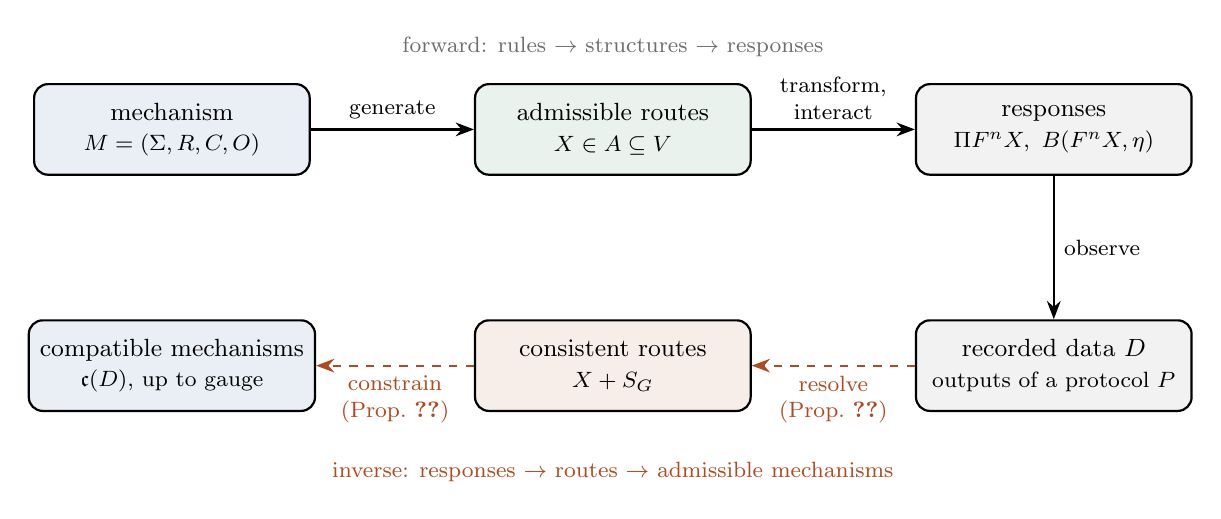
\begin{tikzpicture}[x=1cm,y=1cm,>=Stealth,font=\small,
  box/.style={draw,rounded corners=5pt,thick,align=center,inner sep=4pt,minimum width=3.5cm,minimum height=1.15cm}]
 \node[box,fill=cObs!10] (M)  at (0,0)    {mechanism\\{\footnotesize $M=(\Sigma,R,C,O)$}};
 \node[box,fill=cRel!10] (X)  at (5.6,0)  {admissible routes\\{\footnotesize $X\in A\subseteq V$}};
 \node[box,fill=gray!10] (G)  at (11.2,0) {responses\\{\footnotesize $\Pi F^nX,\ B(F^nX,\eta)$}};
 \node[box,fill=cObs!10] (Mc) at (0,-3.0)   {compatible mechanisms\\{\footnotesize $\mathfrak c(D)$, up to gauge}};
 \node[box,fill=cHid!10] (Xc) at (5.6,-3.0) {consistent routes\\{\footnotesize $X+S_G$}};
 \node[box,fill=gray!10] (D)  at (11.2,-3.0){recorded data $D$\\{\footnotesize outputs of a protocol $P$}};
 \draw[->,thick] (M) -- (X) node[midway,above,align=center,font=\footnotesize] {generate};
 \draw[->,thick] (X) -- (G) node[midway,above,align=center,font=\footnotesize] {transform,\\interact};
 \draw[->,thick] (G) -- (D) node[midway,right,align=left,font=\footnotesize] {observe};
 \draw[->,thick,dashed,cHid] (D) -- (Xc) node[midway,below,align=center,font=\footnotesize,cHid] {resolve\\(Prop.~\ref{prop:profile})};
 \draw[->,thick,dashed,cHid] (Xc) -- (Mc) node[midway,below,align=center,font=\footnotesize,cHid] {constrain\\(Prop.~\ref{prop:gauge})};
 \node[font=\footnotesize,cGrey] at (5.6,1.05) {forward: rules $\to$ structures $\to$ responses};
 \node[font=\footnotesize,cHid] at (5.6,-4.35) {inverse: responses $\to$ routes $\to$ admissible mechanisms};
\end{tikzpicture}
\caption{Forward and inverse directions. The forward direction generates structures and responses from rules. The inverse direction can recover a route only up to $S_G$ (Proposition~\ref{prop:profile}) and a mechanism only up to the gauge of Proposition~\ref{prop:gauge}; what it returns is a \emph{class} of compatible mechanisms.}\label{fig:fwdinv}
\end{figure}

\begin{definition}[Observation protocol; observational equivalence of mechanisms]\label{def:protocol}
An \emph{observation protocol} $P=(N,\mathcal P,A)$ consists of a set $N\subseteq\mathbb N$ of iterates, a set $\mathcal P\subseteq V$ of probes, and a set $A\subseteq V$ of admissible routes.
Its output on a realisation $(B,F)$ is $G_P(X)=\bigl((\Pi F^nX)_{n\in N},(B(F^nX,\eta))_{n\in N,\eta\in\mathcal P}\bigr)$, $X\in A$.
Realisations $M_1,M_2$ are \emph{$P$-equivalent}, $M_1\sim_PM_2$, if $G_P^{M_1}(X)=G_P^{M_2}(X)$ for all $X\in A$; if this holds for every protocol declared admissible we write $M_1\sim_{\mathrm{obs}}M_2$.
\end{definition}
Enlarging $N$, $\mathcal P$ or $A$ can only refine $\sim_P$. If $M_1\sim_{\mathrm{obs}}M_2$, no evidence from the declared protocols can separate them, and the most that can be claimed is membership of a class.

\begin{proposition}[Mechanisms are identifiable only up to gauge]\label{prop:gauge}
Let $\dim V<\infty$ and let $g\in GL(V)$ satisfy $\Pi g=\Pi$. For a realisation $M=(B,F)$ put $g\cdot M=(B^g,F^g)$ with $B^g(X,Y)=B(g^{-1}X,g^{-1}Y)$ and $F^g=gFg^{-1}$. Then:
\begin{enumerate}[label=(\alph*)]
\item $\Pi(F^g)^n(gX)=\Pi F^nX$ and $B^g\bigl((F^g)^n(gX),g\eta\bigr)=B(F^nX,\eta)$ for all $X,\eta\in V$ and $n\ge0$. Thus $M$ and $g\cdot M$ produce the same set of responses \emph{when routes and probes are relabelled by $g$ together}.
\item $\dim K$, $\rho_L$, $\rho_R$, $\defic$ and $\dim S_G$ take the same values on $M$ and $g\cdot M$.
\item If $g$ fixes every route of $A$ and every probe of $\mathcal P$, then $M\sim_Pg\cdot M$ for $P=(N,\mathcal P,A)$. Without that condition the fixed-label outputs of $M$ and $g\cdot M$ may differ.
\end{enumerate}
The group $\{g:\Pi g=\Pi\}$ contains every invertible $\id+N$ with $N\in\operatorname{Hom}(V,K)$, so it is non-trivial whenever $K\ne0$.
\end{proposition}
\begin{proof}
(a) $\Pi g=\Pi$ gives $\Pi g^{-1}=\Pi$, and $(F^g)^n=gF^ng^{-1}$; then $\Pi(F^g)^ngX=\Pi gF^nX=\Pi F^nX$ and $B^g(gF^nX,g\eta)=B(F^nX,\eta)$.
(b) $\Pi g=\Pi$ implies $gK\subseteq K$, hence $gK=K$. Also $\Rad_L(B^g)=g\Rad_L(B)$ and $\Rad_R(B^g)=g\Rad_R(B)$, so $K\cap\Rad_{L/R}(B^g)=g\bigl(K\cap\Rad_{L/R}(B)\bigr)$, and $S_{G}(g\cdot M)=gS_G(M)$ by conjugacy of $F$ and $F^g$. All dimensions are preserved. (c) For $X\in A$, $\eta\in\mathcal P$: $\Pi(F^g)^nX=\Pi gF^ng^{-1}X=\Pi F^nX$ and $B^g((F^g)^nX,\eta)=B(F^nX,g^{-1}\eta)=B(F^nX,\eta)$. For the last claim, $\Pi(\id+N)=\Pi$.
\end{proof}
\begin{remark}[Relabelled versus fixed-label equivalence]\label{rem:labels}
Part (a) is an identity between $M$ evaluated at $(X,\eta)$ and $g\cdot M$ evaluated at $(gX,g\eta)$; it is not an identity at fixed labels. Example: $V=\RR^2$, $\Pi(x,y)=x$, $B(X,Y)=y_Xy_Y$, $F=\id$, $g(x,y)=(x,2y)$. At the fixed route and probe $e_y$ the output of $M$ is $1$ while that of $g\cdot M$ is $B(g^{-1}e_y,g^{-1}e_y)=\tfrac14$; at $(ge_y,ge_y)$ it is $1$ again. Hence the $P$-equivalence of Definition~\ref{def:protocol}, which compares outputs at fixed labels, is finer than equivalence up to relabelling, and the two coincide for the gauge elements allowed by (c), which is a sufficient condition; necessity is not claimed. If an experiment names its routes and probes operationally, the $g$ fixing them certainly remain unidentified; if it does not, the full group acts.
\end{remark}
Labels of the unobservable directions of $V$ are therefore identifiable only to the extent that the protocol names routes and probes (Remark~\ref{rem:labels}); the \emph{invariants} of the isomorphism class of $(V,\Pi,B,F)$ over $\Pi$ are. This is what ``relational identity'' can mean operationally: a statement about $\defic$, $S_G$ or $\rho_L$ is meaningful, a statement about which element of $V$ a route ``really is'' is not, unless the protocol names it.

\begin{proposition}[Probe complexity]\label{prop:probe}
Assume $\dim K<\infty$ (e.g.\ $\dim V<\infty$); ``generic'' means outside a proper algebraic subset of $V^m$. Let $\rho_L=\dim K/(K\cap\Rad_L(B))$ and let $\eta_1,\dots,\eta_m\in V$ be probes. The routes of the fibre $X_0+K$ that no probe separates from $X_0$ at $n=0$ are $X_0+K_J$, $K_J=\{Z\in K:B(Z,\eta_j)=0,\ j\le m\}$. Then $\dim K_J\ge\dim K-m$, and for generic probes $\dim K_J=\dim K-\min(m,\rho_L)$. In particular $\rho_L$ generic probes reduce the ambiguity to $K\cap\Rad_L(B)$, which no left probe can resolve, and fewer than $\rho_L$ probes cannot.
\end{proposition}
\begin{proof}
The map $K\to V^{*}$, $Z\mapsto B(Z,\cdot)$, has kernel $K\cap\Rad_L(B)$ and rank $\rho_L$; so $\Lambda=\{B(\cdot,\eta)|_K:\eta\in V\}\subseteq K^{*}$ has dimension $\rho_L$ (the rank of the same matrix, read column-wise).
$K_J$ is the annihilator in $K$ of $m$ elements of $\Lambda$. These span at most $m$ and, generically, $\min(m,\rho_L)$ dimensions. If $m<\rho_L$ then $\dim K_J\ge\dim K-m>\dim K-\rho_L=\dim(K\cap\Rad_L(B))$.
\end{proof}
Since $\rho_L\le\defic$ (Proposition~\ref{prop:deficit}), this is the experimental counterpart of the statement that $\defic$ additional observables restore descent: here $\rho_L$ interaction tests resolve the fibre up to what no test can see.

\subsection{Admissibility as restriction}
\begin{definition}[Admissible set and its fibre differences]
Let $A\subseteq V$ be the set of routes admitted by the constraints $C$ of a mechanism, and put $K_A=\spn\{X-X':X,X'\in A,\ \Pi X=\Pi X'\}\subseteq K$.
\end{definition}
\begin{proposition}[Restriction]\label{prop:fibre}
For $X,X'\in A$, the implication $\Pi X=\Pi X'\Rightarrow B(X,\eta)=B(X',\eta)\ \forall\eta$ holds iff $K_A\subseteq\Rad_L(B)$. The restricted left deficit $\defic_A=\dim K_A/(K_A\cap\Rad_L(B))$ satisfies $\defic_A\le\rho_L$ and can vanish while $\defic>0$.
\end{proposition}
\begin{proof}
By linearity of $B$ in the first slot the implication holds for all pairs iff every generating difference lies in $\Rad_L(B)$, i.e.\ iff $K_A\subseteq\Rad_L(B)$. $K_A/(K_A\cap\Rad_L(B))$ injects into $K/(K\cap\Rad_L(B))$. For the last claim, in Example~\ref{ex:H8} take $A=\{(u,0)\}$: $\Pi$ is injective on $A$, so $K_A=0$ and $\defic_A=0$, whereas $\defic(\Pi,B_H)=3$.
\end{proof}
Restriction is only as informative as the admissibility principle that imposes it is independent of the observations: choosing $A$ to be a section of $\Pi$ removes every obstruction by fiat.

\subsection{What would make a generative description explanatory}
\begin{definition}[Predicted and discriminating responses]\label{def:predict}
Let $P_0$ be a calibration protocol with recorded outputs $D$, and let $\mathfrak c(D)$ be the class of realisations whose $P_0$-output equals $D$.
A realisation $M\in\mathfrak c(D)$ \emph{predicts} the output $q(M)$ of any protocol $P\supsetneq P_0$. The prediction is \emph{discriminating} if $q(M)\ne q(M')$ for some $M'\in\mathfrak c(D)$.
\end{definition}
In Example~\ref{ex:dyn}, $M_1$ and $M_2$ lie in the same class for $P_0=(\{0\},V,V)$; the response $\Pi F$ discriminates them.
Four requirements for a generative \emph{explanation} then have formal counterparts, with one that is methodological:
\begin{center}\small
\begin{tabularx}{\textwidth}{@{}l>{\raggedright\arraybackslash}X>{\raggedright\arraybackslash}X@{}}
\toprule
Requirement & Formal counterpart & Status\\
\midrule
Construction & $(B,F)$ fixed from $M=(\Sigma,R,C,O)$ without importing the target observable & protocol-level condition (pre-registration); not an algebraic statement\\
Restriction & admissible set $A$, fibre differences $K_A$, restricted deficit $\defic_A$ (Prop.~\ref{prop:fibre}) & formal; its force depends on independent justification of $C$\\
Prediction & outputs of $P\supsetneq P_0$ determined by $M\in\mathfrak c(D)$ (Def.~\ref{def:predict}) & formal; the prediction is fixed before validation data are inspected\\
Discrimination & predictions that split $\mathfrak c(D)$ (Ex.~\ref{ex:dyn}) & formal; instance in the abstract model only\\
\bottomrule
\end{tabularx}
\end{center}

\subsection{The proposed principle}
\begin{principle}[Generative characterisation; proposed]\label{princ:gen}
The generative nature of an observable structure is characterised by the admissible mechanisms capable of producing it, together with the transformation, persistence, boundary and interaction relations those mechanisms imply.
Observable identity alone need not determine generative identity; generative explanations become scientifically informative when they constrain or predict observable behaviour beyond the data used to construct them.
\end{principle}
\noindent
This is a proposed foundational principle, \emph{not a theorem}. Its mathematical content in the present model is the following dictionary; the empirical content, whether canonical UNNS recursion supplies independently justified admissibility principles that make such predictions, is not established.
\begin{center}\small
\begin{tabularx}{\textwidth}{@{}>{\raggedright\arraybackslash}p{0.30\textwidth}>{\raggedright\arraybackslash}X>{\raggedright\arraybackslash}p{0.22\textwidth}@{}}
\toprule
Clause of the principle & Formal object here & Status\\
\midrule
admissible mechanisms capable of producing it & compatible class $\mathfrak c(D)$; restriction through $A$, $K_A$ & definitions; whether UNNS rules fix $A$ is open\\
transformation, persistence & $F$; $\Pi F^nX$; $S_G$ (Ex.~\ref{ex:dyn}) & defined; example only\\
interaction & $B(F^nX,\eta)$; $\rho_L$, $\defic$ & defined and proved\\
boundary & not modelled (linear $F$ has no exit from $A$) & \textbf{open} (L7)\\
observable identity does not determine generative identity & Thm.~\ref{thm:quot}; Cor.~\ref{cor:levels}; Ex.~\ref{ex:H8} & proved\\
only a class of mechanisms is identifiable & Prop.~\ref{prop:gauge} & proved\\
informative beyond calibration data & Def.~\ref{def:predict} & definition; no UNNS instance\\
\bottomrule
\end{tabularx}
\end{center}

\begin{remark}[Weak and strong claims]\label{rem:weakstrong}
\emph{Weak claim:} every observable structure has some generative description. In this framework it is vacuous: the realisation $V=O$, $\Pi=\id$ has $K=0$, $\defic=0$ and $S_G=0$ for any $B,F$.
\emph{Strong claim:} a mechanism whose admissibility principles are justified independently of the observations restricts the admissible routes (small $K_A$) and predicts discriminating responses. Nothing in this paper establishes the strong claim for canonical UNNS; the machinery above only makes it precise enough to be tested, and Problem~\ref{prob:strong} records what a test would need.
\end{remark}
%=====================================================================
\section{Reproducible Constructions}\label{sec:repro}
%=====================================================================
Every example above is finite-dimensional or reduces to a finite computation, and has been checked by deterministic scripts delivered with this manuscript: \path{verify_ri.py} (61 checks; the linear framework and the canonical value-fibre count), \path{rgg2.py} (23 checks and 5 data rows; the nonlinear layer) and \path{rgg21.py} (14 checks and 2 data rows; the consolidation of the nonlinear layer: erratum, single-probe theorem, coordinate robustness). This section records the design of the checks and their outcome; the full output, the SHA-256 digests and the listings are in Appendix~\ref{app:tests}.

\subsection{Design}
\begin{itemize}
\item \textbf{Exact arithmetic where the statement is exact.} The Legendre witnesses (Example~\ref{ex:P3}, Table~\ref{tab:legendre}) are computed with rational arithmetic (\texttt{fractions.Fraction}), and the four-route table (Example~\ref{ex:four}) in $\mathbb Q(\sqrt3)$ by a small exact class; the identities $P_3(\tfrac12)=-\tfrac7{16}$, $B_3(X,r(\mathbf e_x))=\tfrac{15}{16}$, $B_5(X,r(\mathbf e_x))=\tfrac{105}{256}$ are tested for equality, not for tolerance.
\item \textbf{Seeded randomised tests for the general theorems.} Theorem~\ref{thm:quot}, Proposition~\ref{prop:deficit}, Proposition~\ref{prop:invol}, and Theorem~\ref{thm:compat} are tested on random finite-dimensional instances (NumPy generator seeded with a fixed integer), in both ``factoring'' and ``generic'' regimes, with the criterion $K\subseteq\Rad_L\cap\Rad_R$ compared against a direct least-squares test for $B=\mathsf P^{\!\top}\bar{\mathsf B}\mathsf P$.
\item \textbf{Response layer.} Proposition~\ref{prop:profile} (the congruence subspace against a direct unobservability computation, and the completeness criterion of Corollary~\ref{cor:levels}(b)), Proposition~\ref{prop:gauge} (gauge invariance of every protocol output and of $\dim S_G,\rho_L,\defic$), Proposition~\ref{prop:probe} (probe counts) and Proposition~\ref{prop:fibre} (restriction) are tested on seeded random instances; Examples~\ref{ex:H8} and~\ref{ex:dyn} are checked directly.
\item \textbf{Rank computation for the obstruction.} For $N=120$ generic points of $S^2$ (fixed seed) the matrix of $B_\ell$ restricted to $\ker\Pi\times V$ is formed and its numerical rank (tolerance $10^{-8}$) is compared with $2\ell+1$, $\ell=1,\dots,7$.
\item \textbf{Nonlinear layer (RGG-2, RGG-2.1).} Everything in \S\ref{sec:nonlinear} is exact integer arithmetic over fibres $F(m)$ for $m\le6000$ (single-probe theorem: all non-empty fibres with $m\le20000$). Each proved statement is tested as stated; counts that are not theorems (one-argument invariance failures, probe resolution under alternative coordinates, the excess on a grid) are reported as data, never as proofs.
\item \textbf{Quarantine of the scope.} No check uses a probability, a quantum state or a Bell inequality, apart from the arithmetic $\frac14(1+C)$ in Table~\ref{tab:legendre}.
\end{itemize}

\subsection{Checks and outcomes}
\begin{table}[t]
\centering\small
\begin{tabularx}{\textwidth}{@{}l>{\raggedright\arraybackslash}X>{\raggedright\arraybackslash}p{0.25\textwidth}@{}}
\toprule
Group & Statement checked & Outcome\\
\midrule
H & Prop.~\ref{prop:H}(a)--(f): $B=-(uu'+vv')$, $\Pi T=\Pi$, $h_{TX}=-h_X$, joint invariance, failure of independent invariance, $\rk\spn\{X-TX\}=3$, witness $B(k,Y)=-2$ & all pass (max float error $<2\times10^{-15}$)\\
Q & Thm.~\ref{thm:quot}: criterion $\Leftrightarrow$ direct factorisation, 300 random instances; one-sided counterexample & 150 factoring, 150 non-factoring; all agree\\
D & Prop.~\ref{prop:deficit}: bounds, matrix formula, minimal completion with $\defic$ rows (and failure with $\defic-1$) & 300 random cases pass\\
L & Thm.~\ref{thm:legendre}: exact witnesses $\ell=1,3,5$; ranks for $\ell\le7$; positivity of $-B_\ell$; odd-$\ell$ sign reversal & ranks $0,5,7,9,11,13,15$ $=2\ell+1$ for $\ell\ge2$; $-B_\ell\succeq0$\\
I & Prop.~\ref{prop:invol} and Thm.~\ref{thm:compat}: 200 random involutions, block structure and compatibility; coinvariant gap $\dim V_-^{\otimes2}=9$ & all pass\\
P & Example~\ref{ex:perm}, $n=5$: dimension of joint-invariant forms $=2$, independent-invariant forms $=1$; (H2); $\defic=4$ & $2,\,1$; pass; $4$\\
C & \S\ref{sec:closure}: ideal Helmholtz projector per Fourier mode ($\mathbf k=(1,2)$) & idempotent; $R$ involution; joint but not independent invariance; $\defic=1$\\
G & Remark~\ref{rem:gct}: $c_3(d)=-P_3(\cos d)$ satisfies $c(0)=-1$, evenness, $c(d+\pi)=-c(d)$, $|c|\le1$ & pass (41 sample angles)\\
F & Example~\ref{ex:four}: Gram matrices of $B_1,B_3$ on four routes; $G_1k=0$, $G_3k=(\tfrac{15}{16},\tfrac{5\sqrt3}{16},0,-\tfrac{15}{16})^{\!\top}$ & exact over $\mathbb Q(\sqrt3)$; pass\\
S & Prop.~\ref{prop:self}: $Q$ descends iff $B$ descends (100 random symmetric forms); Prop.~\ref{prop:sections}: induced pairing $-\tfrac12s^{\!\top}(\mathsf I+H^{\!\top}H)s'$ & pass\\
R & \S\ref{sec:response}: Props.~\ref{prop:profile}, \ref{prop:gauge}, \ref{prop:probe}, \ref{prop:fibre} (300/300/200/200 random instances); Ex.~\ref{ex:H8} witness $B(X,Y)=-1$, $B(X',Y)=0$, $S_G$ of dimensions $0$ and $3$; Ex.~\ref{ex:dyn} (shear separates, identity does not); trivial realisation $V=O$ & all pass\\
N & Prop.~\ref{prop:nest}: identity $M\perp N=M(N+1)^2/N$ (exact, $59\times59$); fibre of $72$ is $\{(18,1),(16,2),(10,5)\}$; $235$ multi-route values for $M\le200$, $N\le40$; Cor.~\ref{cor:fibre}: $R(m)$ formula for all $m\le3000$, squarefree characterisation, integer iff $N\mid M$ & all pass (exact arithmetic)\\
\midrule
RGG-2 & \S\ref{sec:nonlinear} (\path{rgg2.py}): order structure and antichain fibres; join value $m(L/g)^2$; universal separation; $D$ as weighted $\ell^1$ metric, triangle inequality, fibre $=$ box minus origin, diameter; joint covariance, isometry of $D$, step cost $2\log q$; one-argument invariance failure ($5098/10304$); fibre connectivity; geodesic $=D$ ($3581$ pairs); set deficit of $\vj$ and of the product; excess; meet and mixed operations; occurrence-coordinate closure & 23 pass, 0 fail; 5 data rows\\
RGG-2.1 & \S\ref{sec:nlprobe}, \S\ref{sec:nlrobust}, \S\ref{sec:nlalt} (\path{rgg21.py}): erratum (admissibility of mixed operations; join-semilattice; lattice after adjoining $(m,1)$); single-probe theorem and decoding on $7840$ non-empty fibres ($m\le20000$); probe family; monotonicity and separation in three coordinate charts & 14 pass, 0 fail; 2 data rows\\
\bottomrule
\end{tabularx}
\caption{Summary of the verification. All $61+23+14=98$ checks pass (plus $5+2$ data rows that are reported, not asserted); each script exits with status $0$. Raw output and digests: Appendix~\ref{app:tests}.}\label{tab:checks}
\end{table}

\subsection{What was not re-run}
The GCT repository contains its own regression suites (for instance \path{tests/test_gct_joint_origin_v002.py}). Those were not executed as part of this work and are not relied upon. The route-test analysis that first produced the Legendre counterexample and the $(s,h)$ decomposition is available to us as a transcript~\cite{G9}; the package of tests that it reports for its own two-state recurrent realisation was \emph{not} among the files provided, so no claim about that realisation is verified here. The models of this paper are the abstract algebraic ones defined above, and the verification concerns them only.

%=====================================================================
\section{Implications for UNNS}\label{sec:unns}
%=====================================================================
This section relates the results to canonical UNNS. It keeps three kinds of statement apart: a \emph{proven consequence} (a statement about canonical UNNS objects that follows by proof from adopted definitions alone), a \emph{conditional consequence} (valid for any interaction or transformation that is specified independently and satisfies a stated hypothesis), and a \emph{proposed extension} (a definition or principle introduced here). It asserts no property of canonical UNNS recursion beyond the first kind. The nonlinear results of \S\ref{sec:nonlinear} are conditional in the second sense on one proposed operation, and are stated there with that status.

\subsection{Canonical UNNS: structural commitments and mathematical consequences}\label{sec:canon}
Not having proved a theorem about the interaction of a canonical mechanism does not make the results irrelevant to UNNS. The entry grammar commits UNNS to a particular reading of a number: a value is structurally meaningful as a \emph{generated occurrence}, carrying a rule, a position, a route, a boundary and a status, so that a value is read together with its rule and route~\cite{G11,G12}. The question treated here, what is lost when only the value is retained, is therefore a question about canonical UNNS. The correspondence below states which features are inherited, which are formal representations, and which are new.
\begin{center}\small
\begin{tabularx}{\textwidth}{@{}>{\raggedright\arraybackslash}p{0.25\textwidth}>{\raggedright\arraybackslash}p{0.27\textwidth}>{\raggedright\arraybackslash}X@{}}
\toprule
Canonical UNNS concept & Object in this manuscript & Origin\\
\midrule
Generated occurrence $(M,N)$ with rule, route, boundary, status & elementary route $r(M,N)$; route space $V=F(E)$ & concept inherited; the free linear span is a \emph{formal representation} introduced here\\
Generated value $M\perp N$ & observation $\Pi$ & value inherited; linear extension formal\\
Same occurrence (same rule, position, route) & generative identity, equality in $V$ & inherited on $E$; canonicalisation relations for combinations: new, unspecified\\
Admissibility, five criteria & admissible set $A$, fibre differences $K_A$ & criteria inherited; their use as restriction is new\\
Recursive operation & transformation operator $F$ & concept inherited; a linear $F$ for the nest rule is not specified (open)\\
Structure-preserving morphism & refinement family $\mathcal T$, $\Pi T=\Pi$ & concept inherited; identification with $\Pi$-preserving maps new\\
Generative interaction & pairing $B$ & \textbf{not defined in the entry grammar~\cite{G11}}; must be specified independently (open)\\
Lost relational distinction & $K/(K\cap\Rad B)$ & formal; conditional on $B$\\
\bottomrule
\end{tabularx}
\end{center}
\begin{proposition}[Value does not determine route; proven consequence]\label{prop:nest}
The nest operation satisfies $M\perp N=MN+M/N+2M=M(N+1)^2/N$. Among positive integer pairs, the value $72$ is generated by exactly three occurrences, $(M,N)=(18,1),(16,2),(10,5)$. Each lies on an integer-anchor route ($M=kN$ with $k=18,8,2$), for three different nests and three different boundary conditions $N\mid M$.
\end{proposition}
\begin{proof}
The identity is algebra. For $72$ we need $M=72N/(N+1)^2\ge1$, i.e.\ $N\le69$; checking $N\le69$ leaves exactly $N=1,2,5$ with $M=18,16,10$, and $k(N+1)^2=72$ in each case. (Exact enumeration: Appendix~\ref{app:tests}.)
\end{proof}
Thus the observable value $72$ does not determine the generated occurrence: the three occurrences differ in generative identity (rule parameter $N$, position $M$) and in boundary ($N\mid M$ for $N=1,2,5$), although all three share the status of anchor. In the linear representation, $r(10,5)-r(18,1)$ and $r(10,5)-r(16,2)$ lie in $K=\ker\Pi$. This is a statement about canonical objects (the set-level non-injectivity of the value map) and needs no linear model. By direct enumeration $235$ values with $M\le200$, $N\le40$ have at least two occurrences.
\begin{corollary}[Nest fibre multiplicity]\label{cor:fibre}
For positive integers $M,N$, $M\perp N$ is an integer iff $N\mid M$, and then $M\perp N=k(N+1)^2$ with $k=M/N$; in particular every occurrence with an integer value lies on an anchor route, so equal integer values have equal anchor status. For an integer $m\ge1$ the number of positive-integer pairs $(M,N)$ with $M\perp N=m$ is
\[R(m)=\#\{d\ge2:\ d^2\mid m\}=\prod_{p^e\,\Vert\, m}\Bigl(\Bigl\lfloor\frac e2\Bigr\rfloor+1\Bigr)-1 .\]
In particular $R(72)=(1+1)(1+1)-1=3$, and $R(m)=0$ iff $m$ is squarefree: no squarefree integer is an output of the positive-integer nest operation, and every integer divisible by a nontrivial square is an output.
\end{corollary}
\begin{proof}
Since $\gcd(N,(N+1)^2)=1$, $N$ divides $M(N+1)^2$ iff $N\mid M$. Writing $M=kN$ gives $m=k(N+1)^2$, so the occurrences of integer value $m$ correspond bijectively to $d=N+1\ge2$ with $d^2\mid m$ (then $k=m/d^2$). The number of $d\ge1$ with $d^2\mid m=\prod p^e$ is $\prod(\lfloor e/2\rfloor+1)$; remove $d=1$. $R(m)=0$ iff $m$ has no square divisor $>1$. (Checked by enumeration for all $m\le3000$: Appendix~\ref{app:tests}.) The formula concerns integer values; fibres over non-integer values are not covered.
\end{proof}
\par\smallskip\noindent\textbf{Conditional consequence.} For \emph{any} bilinear interaction $B$ on $V$ that is specified independently, Theorem~\ref{thm:quot} says that the interaction of occurrences is determined by their values iff differences of colliding occurrences lie in $\Rad(B)$; a pairing that separates $(18,1)$ from $(10,5)$ against some probe cannot descend to the value. The entry grammar does not define such a pairing, so whether canonical UNNS retains interaction information invisible to the value is \textbf{not demonstrated}. Section~\ref{sec:nonlinear} proves the corresponding statement for a nonlinear joint continuation, which does not require a bilinear $B$, but whose selection by UNNS rules is open (Problem~\ref{prob:select}).
\par\smallskip\noindent\textbf{The bridge.} The research obligation is a map
\[\boxed{\text{canonical mechanism}\ \longrightarrow\ (V,\Pi,B,\mathcal T,F)}\]
constructed for at least one authentic mechanism, with $B$ determined independently of the desired theorem. For the nest rule, the pair $(V,\Pi)$ is supplied by Proposition~\ref{prop:nest}; $F$, $\mathcal T$ and $B$ are not. If the bridge is built, the manuscript can make a direct claim about that mechanism; if not, the results remain model-conditional (Problem~\ref{prob:bridge}). For the nest rule, \S\ref{sec:nonlinear} supplies a nonlinear instance of the bridge in which $\Pi=v$, the refinements are $T_q$ and the joint operation is $\vj$; it is an instance with a \emph{proposed} operation, not yet a derivation from the mechanism's own rules.
\begin{principle}[Scoped statement for the UNNS Substrate; proposed]\label{princ:scoped}
In the UNNS Substrate, the characterisation of generated structures includes their routes, admissibility conditions and transformation histories. Consequently, equality of observable representations alone does not establish equality of generative descriptions. The present work gives a rigorous algebraic criterion for when observational reduction preserves interaction equivalence and when relational distinctions may survive it. Its applicability to a particular canonical mechanism depends on constructing the observation and interaction maps from that mechanism's independently specified rules.
\end{principle}
The first two sentences rest on the adopted grammar and Proposition~\ref{prop:nest}; the third is Theorem~\ref{thm:quot}; the fourth is the conditional consequence above.


\subsection{Structural identity}
The three equivalences of Definition~\ref{def:three} (and, with a transformation operator, the profile equivalence of Definition~\ref{def:profile} between the generative and the observable one) correspond to levels at which a UNNS-style description can speak about a generated occurrence:
\begin{center}\small
\begin{tabularx}{\textwidth}{@{}l>{\raggedright\arraybackslash}X>{\raggedright\arraybackslash}X@{}}
\toprule
Equivalence & Meaning in the route language & Substitution requires\\
\midrule
Generative & same structural identity under declared canonicalisation & nothing (strongest)\\
Observable & same projected observable & $K\subseteq\Rad(B)$ to replace interaction equivalence\\
Interaction & identical pairings with all other routes & $\Rad(B)\subseteq K$ to replace observable equivalence\\
\bottomrule
\end{tabularx}
\end{center}
The point is not that a particular substitution is false but that \emph{none is automatic}. A description that treats ``same observable'' as ``same structure'' is making a compatibility assumption, and Theorem~\ref{thm:quot} states exactly which one.

\subsection{Projection and admissibility}
A projection $\Pi$ is part of the specification of an observable realisation. Two disciplines follow.
\begin{enumerate}[label=(D\arabic*)]
\item \emph{Declare the observation map together with each pairing.} For every interaction $B$ used, either prove $\ker\Pi\subseteq\Rad(B)$ (observable-null compatibility), or report $\defic(\Pi,B)$.
\item \emph{Declare the transformation and the protocol.} A claim about the generative character of a structure names the operator $F$, the iterates and probes used, and the admissible set $A$ (Definition~\ref{def:protocol}); without them only $\Pi$ and $B$ at $n=0$ are specified, and mechanisms that differ in $F$ are indistinguishable (Example~\ref{ex:dyn}).
\item \emph{Do not infer compatibility from joint symmetry.} Joint refinement invariance is what an exchange or relabelling symmetry of \emph{both} arguments delivers; Theorem~\ref{thm:joint} shows that it leaves the internal sector's own interaction untouched. Independent invariance under a family satisfying (H2) is the condition that does the work (Theorem~\ref{thm:compat}).
\end{enumerate}
In the language of the GCT analysis, the \emph{observable-null refinement condition} --- a route combination with no net observable cannot contribute to joint pairings --- was identified as an additional principle not forced by the route and admissibility rules examined there~\cite{G9}. In the present formulation it is precisely $K\subseteq\Rad(B)$, equivalently (under (H2)) independent refinement invariance. Whether canonical UNNS admissibility entails it remains open (Problem~\ref{prob:entail}); this paper supplies the exact form of the question and examples showing that it is not vacuous.

\subsection{Illustration: Operator XVI closure as an observation-like projection}\label{sec:closure}
Chamber XVI states the Closure hypothesis as a Helmholtz decomposition that seals flux divergence in an evolved $\tau$-field~\cite{G7}. We use only the \emph{ideal} $L^2$ projector on a periodic domain, not the Chamber's discrete implementation (whose source audit records a hybrid discrete/spectral symbol and a closure diagnostic that is not a direct projector-idempotence test~\cite{G5}).
Per nonzero Fourier wavevector $\mathbf k\in\RR^2$, the solenoidal projector is $\mathsf P_{\mathbf k}=\mathsf I-\mathbf k\mathbf k^{\!\top}/|\mathbf k|^2$ on the amplitude space $V_{\mathbf k}=\RR^2$; it is idempotent with kernel $K=\spn\{\mathbf k\}$ (longitudinal, i.e.\ gradient, amplitudes). Take $\Pi=\mathsf P_{\mathbf k}$ as the ``observable'' map, the involution $\mathsf R=2\mathsf P_{\mathbf k}-\mathsf I$ (which reverses the longitudinal part), and the $L^2$ pairing $B(X,Y)=X\cdot Y$. Then $\mathsf R$ preserves $\Pi$, $B(\mathsf RX,\mathsf RY)=B(X,Y)$, $B(\mathsf RX,Y)\ne B(X,Y)$ in general, $\Rad(B)=0$ and $\defic=1$.
This is the structure of Proposition~\ref{prop:invol} with $V_+$ the solenoidal and $V_-$ the longitudinal part. In words: the $L^2$ pairing of two fields is invariant under reflecting the compressive component of \emph{both}, but a pairing that depended on the closed field alone would have to ignore the compressive component entirely. This is a formal illustration of the abstract structure; it makes no statement about the numerical behaviour of Chamber XVI.


\subsection{Relational information}
Define the \emph{relational residue} of $(\Pi,B)$ as the quotient $\mathcal R(\Pi,B)=K/(K\cap\Rad B)$, with $\dim\mathcal R=\defic$. It is the part of the generative description that is invisible to $\Pi$ but visible to $B$; in the algebraic sense used here, ``relational information'' that is lost by observation is exactly this residue. We use the word information only in this algebraic sense; no entropy or probability is defined. The compatibility hierarchy (Figure~\ref{fig:hier}) says that under (H1)--(H2) the residue vanishes if and only if the interaction is independently refinement invariant.

\subsection{Possible applications (not validated)}
Questions of the same form --- does an interaction between microscopic configurations depend on them only through a macroscopic variable? --- occur in coarse-grained dynamical systems, multiscale modelling, structural representations and accounts of emergent observables. Example~\ref{ex:perm} is the prototype: a sum observable is complete for interactions invariant under each relabelling separately and incomplete otherwise. We offer the criteria of Theorems~\ref{thm:quot} and~\ref{thm:compat} as candidate tests in such settings, and present these as \emph{possible} applications. No empirical claim is made, and no physical system is analysed.

%=====================================================================
\section{Nonlinear Relational Invariants: Joint Generation, Quotient Obstruction, and Refinement Geometry}\label{sec:nonlinear}
%=====================================================================
Sections~\ref{sec:routes}--\ref{sec:response} work in a linear route space with a bilinear pairing; the only statement about canonical UNNS objects (\S\ref{sec:canon}) is that the nest \emph{value} does not determine the generated \emph{occurrence}.
That statement leaves a gap: it shows that the value map $\Pi$ is not injective on canonical routes, but says nothing about whether the lost distinction can be detected through \emph{relations}, because the entry grammar defines no interaction (\S\ref{sec:canon}).
This section closes part of that gap without leaving the canonical objects and without assuming bilinearity.
It studies one explicit, nonlinear \emph{joint-continuation} operation on anchor routes, the least upper bound $\vj$ in the divisibility order of the nest, and proves what follows from it: universal separation of every collision fibre, an exact relational distance, its identification with minimal refinement cost, a set-theoretic version of the quotient criterion, and a theorem that a single value-dependent probe reconstructs every route of a fibre.

\medskip\noindent
\fbox{\parbox{0.955\textwidth}{\small
\textbf{Central claim, in the form proved here.}
\begin{center}\textbf{Observable equality $\not\Rightarrow$ relational indistinguishability.}\end{center}
Equal nest values do not make two anchor routes indistinguishable once routes may be \emph{jointly continued}: for the least-upper-bound continuation $\vj$, any two distinct routes of one value fibre are separated by the value of their joint continuation with a suitable probe, and the separation has an exact geometry,
\[ D(r,r')=\log\frac{v(r\vj r')}{m}\;=\;\text{minimal refinement-path cost between }r\text{ and }r'.\]
\textbf{What is not claimed.} The consequences of $\vj$ are proved. The independent generative principle that would \emph{select} $\vj$ from the competing operations of \S\ref{sec:nlalt} is \emph{open}; with the componentwise product the same fibres are \emph{not} separated. No physical interaction and no quantum-entanglement mechanism has been derived.}}
\medskip

\paragraph{Status labels.}
\textbf{Proved}: an argument is given in the text. \textbf{Checked}: finite computation by \path{rgg2.py} or \path{rgg21.py} only (Appendix~\ref{app:tests}); not a theorem. \textbf{Proposed}: a definition or choice made here. \textbf{Open}: not settled.

%---------------------------------------------------------------------
\subsection{Setting: anchor routes, fibres, and the join}\label{sec:nlset}
By Corollary~\ref{cor:fibre}, an integer nest output $M\perp N$ has $N\mid M$. Writing $M=kN$ and $d=N+1\ge2$ we have $M\perp N=kd^2$.
An \emph{anchor route} is therefore a pair $r=(k,d)$ of integers $k\ge1$, $d\ge2$, with \emph{value} $v(r)=kd^2$; the occurrence is $(M,N)=(k(d-1),d-1)$, and $(k,d)\leftrightarrow(M,N)$ is a bijection onto anchor occurrences.
For $m\ge1$ the \emph{fibre} is $F(m)=\{r:\ v(r)=m\}=\{(m/d^2,d):\ d\ge2,\ d^2\mid m\}$, and $|F(m)|=R(m)$ (Corollary~\ref{cor:fibre}).
For $m=72$ the fibre is $\{(18,2),(8,3),(2,6)\}$, the occurrences $(18,1),(16,2),(10,5)$ of Proposition~\ref{prop:nest}.
Field occurrences ($N\nmid M$) have non-integer values and are \emph{excluded} from this section (see \S\ref{sec:nlstatus}).

\begin{definition}[Divisibility order and joint continuation; proposed]\label{def:nljoin}
Order anchor routes by $r\le s$ iff $k_r\mid k_s$ and $d_r\mid d_s$. The \emph{joint continuation} is
\[ r\vj s=\bigl(\lcm(k_r,k_s),\ \lcm(d_r,d_s)\bigr). \]
\end{definition}
\noindent Definition~\ref{def:nljoin} is a proposal: it is the least route that extends both arguments in the divisibility structure of the nest. It is not given by the entry grammar~\cite{G11,G12}, and \S\ref{sec:nlalt} shows what changes if another operation is used.

\begin{lemma}[Order structure; proved]\label{lem:nlorder}
$\vj$ is the least upper bound of $r,s$ for $\le$ (hence commutative, associative and idempotent); $v(r)\mid v(r\vj s)$ and $v(s)\mid v(r\vj s)$; and $v$ is strictly increasing in each coordinate, so every fibre $F(m)$ is an antichain.
\end{lemma}
\begin{proof}
The componentwise least common multiple is the least upper bound for componentwise divisibility. Divisibility of values is immediate from $v=kd^2$. If $r\le r'$ and $v(r)=v(r')$ then $(k'/k)(d'/d)^2=1$ with both ratios positive integers, so $r=r'$.
\end{proof}

%---------------------------------------------------------------------
\subsection{Join structure and universal fibre separation}\label{sec:nlsep}
\begin{theorem}[Join value; proved]\label{thm:nljoin}
Let $r=(m/d^2,d)$ and $r'=(m/d'^2,d')$ lie in $F(m)$, and put $g=\gcd(d,d')$, $L=\lcm(d,d')$. Then $\lcm(k,k')=m/g^2$ and
\[ v(r\vj r')\;=\;m\Bigl(\frac Lg\Bigr)^{2}. \]
\end{theorem}
\begin{proof}
Fix a prime $p$ with $\nu_p(m)=e$, $\nu_p(d)=a$, $\nu_p(d')=a'$. Then $\nu_p(k)=e-2a$ and $\nu_p(k')=e-2a'$, so $\nu_p\lcm(k,k')=\max(e-2a,e-2a')=e-2\min(a,a')=\nu_p(m/g^2)$. Hence $v(r\vj r')=\lcm(k,k')L^2=(m/g^2)L^2$.
\end{proof}
\noindent Example: in $F(72)$, $(18,2)\vj(8,3)=(72,6)$ of value $2592=72\cdot6^2$; $(18,2)\vj(2,6)=(18,6)$ of value $648=72\cdot3^2$; $(8,3)\vj(2,6)=(8,6)$ of value $288=72\cdot2^2$.

\begin{corollary}[Universal fibre separation; proved]\label{cor:nlsep}
If $r\neq r'$ lie in $F(m)$ then $v(r\vj r')>m=v(r\vj r)$. Consequently the value of the joint continuation with probe $s=r$ distinguishes $r$ from every other route of its fibre, and every non-trivial nest fibre is resolved at the level of joint-continuation values.
\end{corollary}
\begin{proof}
Since $k=m/d^2$, $r\neq r'$ forces $d\ne d'$, hence $L>g$ and $v(r\vj r')=m(L/g)^2>m$; while $r\vj r=r$ has value $m$.
\end{proof}
\noindent This is a consequence of the definition of $\vj$ and of the fact that the join is a lattice-theoretic upper bound; it is not independent evidence that canonical UNNS routes interact.

\paragraph{Contrast with the product.}
Let $r\times s=(k_rk_s,d_rd_s)$ (componentwise product, \emph{proposed}). Then $v(r\times s)=v(r)v(s)$ exactly, so $v(r\times s)$ depends only on the values $v(r),v(s)$: the product descends to the value and separates nothing. Hence the separation of Corollary~\ref{cor:nlsep} is a property of $\vj$, not of joint continuation as such (see \S\ref{sec:nlquot}).

%---------------------------------------------------------------------
\subsection{Relational distance and fibre geometry}\label{sec:nldist}
\begin{definition}[Relational distance; proposed as a name]\label{def:nldist}
For $r,r'\in F(m)$ let
\[ D(r,r')=\log\frac{v(r\vj r')}{m}=2\log\frac Lg=2\sum_p\bigl|\nu_p(d)-\nu_p(d')\bigr|\log p. \]
\end{definition}
\begin{theorem}[Fibre geometry; proved]\label{thm:nlgeom}
Put $b_p=\lfloor\nu_p(m)/2\rfloor$. The map $d\mapsto(\nu_p(d))_p$ identifies $F(m)$ with $\prod_p\{0,\dots,b_p\}\setminus\{0\}$ (the box of exponent vectors, origin $d=1$ removed), and $D$ is the weighted $\ell^1$ metric with weights $2\log p$. In particular $D$ is a metric, $|F(m)|=\prod_p(b_p+1)-1=R(m)$, and
\[ \operatorname{diam}F(m)=\begin{cases}2\sum_p b_p\log p,&\text{if at least two }b_p\ge1,\\ 2(b_p-1)\log p,&\text{if exactly one }b_p\ge1.\end{cases} \]
\end{theorem}
\begin{proof}
$d^2\mid m$ iff $0\le\nu_p(d)\le b_p$ for all $p$, and $d\ge2$ iff the vector is nonzero; the displayed formula for $D$ is the weighted $\ell^1$ distance, hence a metric. For the diameter, the full box has diameter $2\sum b_p\log p$, attained at opposite corners. If at least two primes have $b_p\ge1$, split the relevant primes into two non-empty groups; the point equal to $b$ on the first group and $0$ elsewhere and the point equal to $b$ on the second group and $0$ elsewhere are both non-zero and at the full distance. If exactly one prime is relevant, the points are $1,\dots,b_p$ on a line and the diameter is $(b_p-1)2\log p$.
\end{proof}
\noindent The diameter formula and the triangle inequality on all fibre triples are also machine-checked for $m\le6000$ (\path{rgg2.py}, checks~3b, 4, 4b).

%---------------------------------------------------------------------
\subsection{Refinement geometry}\label{sec:nlref}
For a prime $q$ set $T_q(k,d)=(k/q^2,\,dq)$ whenever $q^2\mid k$. It \emph{preserves the value} ($k/q^2\cdot d^2q^2=kd^2$); its inverse is $(k,d)\mapsto(kq^2,d/q)$ when $q\mid d$ and $d/q\ge2$. These are the \emph{refinements} of the anchor setting, the analogue of the family $\mathcal T$ of \S\ref{sec:refinement}: they preserve $\Pi=v$ and move a route within its fibre. Give the step $T_q^{\pm1}$ the \emph{cost} $2\log q$.

\begin{theorem}[Joint covariance versus independent invariance; proved, with one checked count]\label{thm:nlcov}
If $T_qr$ and $T_qs$ are defined, then $T_qr\vj T_qs=T_q(r\vj s)$. Consequently the value $v(r\vj s)$ and the distance $D$ are invariant under \emph{joint} refinement of both arguments, and one step moves a route by $D(T_qr,r)=2\log q$. Invariance under refinement of only \emph{one} argument fails: $v(T_qr\vj s)\ne v(r\vj s)$ in $5098$ of $10304$ tested cases (checked, \path{rgg2.py} check~5d).
\end{theorem}
\begin{proof}
$\lcm(k/q^2,k'/q^2)=\lcm(k,k')/q^2$ and $\lcm(dq,d'q)=q\,\lcm(d,d')$, so the joint continuation of the refined routes is the refinement of the joint continuation, and $T_q$ preserves value. For the step cost, $T_qr$ and $r$ differ by one in $\nu_q(d)$, so $D=2\log q$.
\end{proof}
\noindent This is the nonlinear counterpart of Result~II: joint refinement covariance holds, one-argument invariance fails, and the value alone does not determine the relational behaviour.

\begin{theorem}[Relational distance equals minimal refinement cost; proved, checked on $3581$ pairs]\label{thm:nlgeo}
For $r,r'\in F(m)$, the minimal total cost of a chain of refinement steps (and inverses) from $r$ to $r'$ equals $D(r,r')$. Hence three descriptions coincide: the logarithmic join excess, the weighted $\ell^1$ distance of exponent vectors, and the minimal refinement-path cost.
\end{theorem}
\begin{proof}
A step changes one exponent $\nu_p(d)$ by $\pm1$ at cost $2\log p$, so any chain costs at least $\sum_p|\nu_p(d)-\nu_p(d')|\,2\log p=D$. Conversely, the exponent vector $\max(\nu(d),\nu(d'))$ satisfies $\le b$ coordinatewise and is non-zero, so it is a fibre route (namely $d=\lcm(d,d')$); the chain $d\to\lcm(d,d')\to d'$ stays inside the fibre (it never reaches $d=1$) and costs exactly $D$.
\end{proof}
\noindent The statement that the generated equivalence of the refinements is the value equivalence on anchors (every fibre is connected by prime refinements) is the content of the same argument and is checked in \path{rgg2.py} (check~5e). It is the analogue of hypothesis (H2) of \S\ref{sec:compat}.

%---------------------------------------------------------------------
\subsection{A set-theoretic quotient criterion without bilinearity}\label{sec:nlquot}
Theorem~\ref{thm:quot} uses linearity to speak of radicals. For an arbitrary joint operation the same idea survives in set-theoretic form. Let $\Pi$ be an observation, $\sim_\Pi$ the induced equivalence, and $J$ a (possibly set-valued) joint operation, with $\Pi_*J(r,s)$ the image set. Say that $J$ \emph{descends} to $\Pi$ if $r\sim_\Pi r'$ implies $\Pi_*J(r,s)=\Pi_*J(r',s)$ for all $s$, and likewise in the second slot.

\begin{theorem}[Set-theoretic Quotient Criterion; proved]\label{thm:nlsetq}
Let $\mathcal T$ be a family of refinements and $\sim_{\mathcal T}$ the equivalence relation generated by the pairs $(r,Tr)$. Assume $\sim_{\mathcal T}\,=\,\sim_\Pi$. Then $J$ descends to $\Pi$ if and only if $\Pi_*J(Tr,s)=\Pi_*J(r,s)$ and $\Pi_*J(r,Ts)=\Pi_*J(r,s)$ for all generating $T$, $r$ and $s$.
\end{theorem}
\begin{proof}
Necessity is immediate because $r\sim_\Pi Tr$. For sufficiency, fix $s$. The relation $\{(r,r'):\Pi_*J(r,s)=\Pi_*J(r',s)\}$ is an equivalence relation; it contains $\sim_{\mathcal T}$ as soon as it contains the generating pairs $(r,Tr)$, and $\sim_{\mathcal T}=\sim_\Pi$ by assumption. The same argument applies in the second slot.
\end{proof}
This is the nonlinear analogue of the Refinement-Compatibility Theorem~\ref{thm:compat}: the hypothesis $\sim_{\mathcal T}=\sim_\Pi$ is the analogue of (H2), the one-argument invariance on generators is the analogue of independent refinement invariance.

\begin{corollary}[Application to anchors; proved / checked]\label{cor:nlapp}
For the value observation the hypothesis $\sim_{\mathcal T}=\sim_{v}$ holds (Theorem~\ref{thm:nlgeo}). The product $\times$ satisfies the one-argument invariance (it descends, \path{rgg2.py} check~6c), whereas $\vj$ violates it (Theorem~\ref{thm:nlcov}) and therefore does not descend to the value.
\end{corollary}

\begin{definition}[Set deficit; proposed]\label{def:nlsetdef}
For a fibre $F(m)$ let $\kappa(m)$ be the number of classes of the largest $J$-congruence contained in $\sim_\Pi$, and $\defic_{\rm set}(m)=\kappa(m)-1$.
\end{definition}
\noindent Then $\defic_{\rm set}(m)=R(m)-1$ for $\vj$, because by Corollary~\ref{cor:nlsep} all routes of a fibre are pairwise separated, and $\defic_{\rm set}(m)=0$ for $\times$ with value observation (checked on fibres with $m\le3000$ against a finite set of probes; \path{rgg2.py} checks~6, 6b). The set deficit counts classes rather than dimensions and is not claimed to equal the linear deficit of Proposition~\ref{prop:deficit} in any setting; the comparison is an analogy, not a theorem of this paper.

%---------------------------------------------------------------------
\subsection{Single-probe fibre reconstruction}\label{sec:nlprobe}
Corollary~\ref{cor:nlsep} uses a probe that depends on the route to be separated. A stronger statement holds: one \emph{fixed} probe per fibre resolves the whole fibre, and the route can be \emph{decoded} from a single value. Let
\[ h(m)=\prod_p p^{\lfloor\nu_p(m)/2\rfloor},\qquad s_m=\bigl(m/h(m)^2,\ h(m)\bigr). \]
\begin{theorem}[Single-Probe Fibre Reconstruction; proved]\label{thm:nlsingle}
$F(m)\ne\varnothing$ iff $m$ is not squarefree iff $h(m)\ge2$, and then $s_m\in F(m)$. For every $r=(m/d^2,d)\in F(m)$,
\[ r\vj s_m=\bigl(m/d^2,\ h(m)\bigr),\qquad v(r\vj s_m)=m\Bigl(\frac{h(m)}{d}\Bigr)^{2}. \]
Hence the \emph{decoding formula}
\[ d=h(m)\sqrt{\frac{m}{v(r\vj s_m)}},\qquad r=(m/d^2,d), \]
recovers the entire route $r$ from the single value $v(r\vj s_m)$, and $r\mapsto v(r\vj s_m)$ is injective on $F(m)$.
\end{theorem}
\begin{proof}
$d^2\mid m$ implies $\nu_p(d)\le\lfloor\nu_p(m)/2\rfloor$ for every $p$, so $d\mid h(m)$; in particular $h^2\mid m$, and if $h\ge2$ then $s_m=(m/h^2,h)$ is an admissible route of value $m$. Since $d\mid h$ we have $\lcm(d,h)=h$, and since $m/h^2$ divides $m/d^2$ we have $\lcm(m/d^2,m/h^2)=m/d^2$. Hence $r\vj s_m=(m/d^2,h)$ and its value is $(m/d^2)h^2=m(h/d)^2$. Solving for $d$ gives the decoding formula. The equivalences at the start: $h(m)\ge2$ iff some $\nu_p(m)\ge2$ iff $m$ is not squarefree iff $R(m)\ge1$.
\end{proof}
\noindent Example: $h(72)=6$, $s_{72}=(2,6)$, and the joint values with $(18,2)$, $(8,3)$, $(2,6)$ are $648$, $288$, $72$; decoding gives $d=6\sqrt{72/648}=2$, $d=6\sqrt{72/288}=3$, $d=6$. The theorem is checked on all $7840$ non-empty fibres with $m\le20000$ (\path{rgg21.py}, checks~B1--B5).

\begin{corollary}[Probe family; proved]\label{cor:nlfamily}
Any probe $s=(k_s,d_s)$ with $h(m)\mid d_s$ and $k_s\mid m/h(m)^2$ resolves $F(m)$: for every route of the fibre $\lcm(d,d_s)=d_s$ and $\lcm(m/d^2,k_s)=m/d^2$, so $v(r\vj s)=(m/d^2)\,d_s^2$, which is injective in $d$. The probe need not lie in the fibre.
\end{corollary}
\noindent The condition is \emph{sufficient and not claimed necessary}: in a $12\times12$ grid of probes with $m\le3000$, $13238$ of $45672$ (fibre, probe) pairs resolve the fibre while only $1146$ satisfy the condition (\path{rgg21.py}, data row B7). Note also that $s_m$ depends on $m$: it is one probe per fibre, not a universal probe.

%---------------------------------------------------------------------
\subsection{Coordinate-robust separation and relational excess}\label{sec:nlrobust}
The exact formulas of \S\ref{sec:nlsep}--\ref{sec:nlprobe} are specific to the coordinates $(k,d)$, in which the value is $kd^2$. The \emph{phenomenon} of separation is not.
\begin{lemma}[Coordinate-robust separation; proved]\label{lem:nlrobust}
Let anchor routes carry coordinates in which a value $v$ is strictly increasing in each coordinate, and let $J$ be a joint operation with $J(r,s)\ge r,s$ coordinatewise and $J(r,r)=r$. If $r\ne r'$ and $v(r)=v(r')$, then $v(J(r,r'))>v(r)$.
\end{lemma}
\begin{proof}
If $J(r,r')=r$, then $r'\le r$ coordinatewise; with $v(r')=v(r)$ strict monotonicity forces $r'=r$, a contradiction. So $J(r,r')\ge r$ and $\ne r$, and strict monotonicity gives $v(J(r,r'))>v(r)$.
\end{proof}
The lemma applies to the join in $(k,d)$, to the join in $(k,N)$ with $N=d-1$, and to the join in occurrence coordinates $(M,N)$, where the value $M(N+1)^2/N$ is strictly increasing in $M$ and in $N\ge1$; the occurrence join is anchor-closed because $\lcm(N,N')\mid\lcm(M,M')$ whenever $N\mid M$ and $N'\mid M'$.
Strict monotonicity in the three charts and the resulting separation are checked on $2745$ same-value pairs ($m\le6000$) (\path{rgg21.py}, checks~C1, C2; \path{rgg2.py}, check~9e).
Two limits must be recorded. The formulas of Theorems~\ref{thm:nljoin}--\ref{thm:nlgeo} are specific to $(k,d)$. And that the single probe $s_m$ also resolves every fibre under the other two joins is only \emph{checked} ($693/693$ fibres, \path{rgg21.py}, data row C3), not proved.
Lemma~\ref{lem:nlrobust} has a sobering corollary for interpretation: because every upper-bound-type join separates, the \emph{existence} of separation is weak evidence that $\vj$ in particular is distinguished. It supports the phenomenon, not the choice of operation.

\begin{definition}[Relational excess; proposed]\label{def:nlexcess}
For anchor routes $r,s$ put $\varepsilon(r,s)=v(r\vj s)/\lcm\bigl(v(r),v(s)\bigr)$.
\end{definition}
\begin{proposition}[Excess is an integer, equals $1$ on comparable routes, and is not a function of values; proved]\label{prop:nlexcess}
$\varepsilon(r,s)$ is a positive integer; $\varepsilon(r,s)=1$ if $r\le s$ or $s\le r$; and $\varepsilon$ is not a function of $(v(r),v(s))$.
\end{proposition}
\begin{proof}
By Lemma~\ref{lem:nlorder}, $v(r)$ and $v(s)$ both divide $v(r\vj s)$, hence so does their least common multiple. If $r\le s$ then $r\vj s=s$ and $v(r)\mid v(s)$, so both numerator and denominator equal $v(s)$. For the last claim, take the values $4$ and $36$: $F(4)=\{(1,2)\}$ and $F(36)=\{(9,2),(4,3),(1,6)\}$. Then $(1,2)\vj(9,2)=(9,2)$ has value $36$ and $\varepsilon=1$, whereas $(1,2)\vj(4,3)=(4,6)$ has value $144$ and $\varepsilon=144/36=4$.
\end{proof}
\noindent On the tested grid of routes $1\le k\le24$, $2\le d\le24$ the script finds $35687$ value pairs admitting more than one excess (\path{rgg2.py}, check~7). Thus the joint continuation carries route-level information invisible to the two values: the nonlinear counterpart of a positive deficit, obtained without assuming any bilinear $B$.

%---------------------------------------------------------------------
\subsection{Adversarial alternatives and the erratum}\label{sec:nlalt}
The choice of $\vj$ must be tested against its competitors.
\begin{itemize}
\item \textbf{Meet.} $r\wedge s=(\gcd(k,k'),\gcd(d,d'))$ is \emph{partial}: it leaves the anchor domain when $\gcd(d,d')=1$, which happens for $501$ of $2745$ same-value pairs ($m\le6000$). When defined for $r,r'\in F(m)$, $v(r\wedge r')\,v(r\vj r')=m^2$ (proved by the exponent computation of Theorem~\ref{thm:nljoin}; checked).
\item \textbf{Mixed operations.} $(\lcm k,\gcd d)$ and $(\gcd k,\lcm d)$ preserve the value on a fibre: they return $(m/g^2,g)$ and $(m/L^2,L)$, the ``meet'' and ``join'' of the exponent box \emph{inside} the fibre. On foreign probes both leak heavily (checked, data row 9c).
\item \textbf{Other coordinates.} Joins in $(k,N)$ and $(M,N)$ separate all tested pairs (Lemma~\ref{lem:nlrobust}) but with different value formulas.
\item \textbf{Product.} $\times$ is a value homomorphism: it descends and separates nothing (\S\ref{sec:nlsep}).
\end{itemize}

\paragraph{Erratum to the RGG-2 note (not an error in manuscript v2).}
The RGG-2 note stated that the mixed operations stay in the fibre and therefore that \emph{the fibre is a lattice}. That statement is false on the anchor domain $d\ge2$. The mixed operation $(\lcm k,\gcd d)=(m/g^2,g)$ is inadmissible exactly when $g=\gcd(d,d')=1$: for instance $(18,2)$ and $(8,3)$ would map to $(72,1)$, i.e.\ $N=0$, outside the nest ($501$ of $2745$ same-value pairs for $m\le6000$; \path{rgg21.py}, checks~A1--A5). The correct statement is:
\begin{proposition}[Fibre order; proved, checked]\label{prop:nlerratum}
Order $F(m)$ by divisibility of $d$. Then $F(m)$ is a \emph{join-semilattice} with least upper bound $(\gcd k,\lcm d)=(m/L^2,L)$, which is always admissible and lies in $F(m)$; it is a lattice only after adjoining the formal route $(m,1)$ (value $m$, $d=1$), when it becomes the full exponent box $\prod_p\{0,\dots,b_p\}$. Pairs with $\gcd(d,d')=1$ have no common lower bound inside $F(m)$.
\end{proposition}
\begin{proof}
Per prime, $d\mapsto\nu_p(d)$ identifies $F(m)$ with the box minus the origin. The coordinatewise maximum of two non-zero vectors is non-zero, so the least upper bound exists in the fibre. The coordinatewise minimum is non-zero iff the two vectors share a prime of positive exponent, i.e.\ iff $\gcd(d,d')\ge2$; for $\gcd(d,d')=1$ any common lower bound would be the origin. Adjoining the origin gives the full box, a lattice.
\end{proof}
\noindent The principal results of RGG-2 (Theorems~\ref{thm:nljoin}--\ref{thm:nlgeo}, \ref{thm:nlsetq}) are unaffected: they use the join, which stays inside the fibre, and the path in Theorem~\ref{thm:nlgeo} avoids $d=1$. The RGG-2 check~9b verified the algebra of the mixed operations but not admissibility; \path{rgg21.py} closes that gap. Manuscript v2 contains none of these statements.

%---------------------------------------------------------------------
\subsection{Status of the nonlinear layer and what remains open}\label{sec:nlstatus}
\begin{center}\small
\begin{tabularx}{\textwidth}{@{}>{\raggedright\arraybackslash}X>{\raggedright\arraybackslash}p{0.24\textwidth}@{}}
\toprule
Statement & Status\\
\midrule
$\vj$ is the least upper bound; fibres are antichains (Lemma~\ref{lem:nlorder}) & proved\\
$v(r\vj r')=m(L/g)^2$; universal fibre separation (Thm.~\ref{thm:nljoin}, Cor.~\ref{cor:nlsep}) & proved\\
$D$ is a weighted $\ell^1$ metric; fibre $\cong$ box minus origin; diameter (Thm.~\ref{thm:nlgeom}) & proved\\
Joint refinement covariance; $D$ joint-invariant (Thm.~\ref{thm:nlcov}) & proved\\
One-argument invariance fails ($5098/10304$) & checked\\
$D$ equals minimal refinement-path cost (Thm.~\ref{thm:nlgeo}) & proved; checked on $3581$ pairs\\
Set-theoretic Quotient Criterion (Thm.~\ref{thm:nlsetq}) & proved\\
Single-Probe Fibre Reconstruction and decoding (Thm.~\ref{thm:nlsingle}) & proved; checked on $7840$ fibres\\
Probe family (Cor.~\ref{cor:nlfamily}) & proved (sufficient only)\\
Coordinate-robust separation (Lemma~\ref{lem:nlrobust}) & proved\\
$s_m$ resolves fibres under $(k,N)$, $(M,N)$ joins & checked only ($693/693$)\\
Excess $\varepsilon$ integral, $1$ on comparable routes, not a function of values (Prop.~\ref{prop:nlexcess}) & proved\\
Fibre is a join-semilattice, a lattice after adjoining $(m,1)$ (Prop.~\ref{prop:nlerratum}) & proved; erratum to RGG-2\\
An independent UNNS generative constraint that \emph{selects} $\vj$ (Problem~\ref{prob:select}) & \textbf{open}\\
A bilinear or tropical representation of $\vj$ (Problem~\ref{prob:tropical}) & \textbf{open}\\
Joint continuation for field (non-anchor) occurrences (Problem~\ref{prob:field}) & \textbf{open}\\
Physical interaction, quantum entanglement, Bell-type correlations & \textbf{not claimed, not derived}\\
\bottomrule
\end{tabularx}
\end{center}
\paragraph{Relation to the linear framework.}
In exponent coordinates the join is the coordinatewise \emph{maximum}, a tropical operation; it is not bilinear, so none of Theorems~\ref{thm:quot}--\ref{thm:compat} applies to it directly, and the nonlinear results above are not corollaries of the linear ones. What carries over is the structure of the argument: an observation (the value), a family of value-preserving refinements generating the observable equivalence (the analogue of (H1)--(H2)), joint covariance without independent invariance, and a quotient criterion (Theorem~\ref{thm:nlsetq}) saying when the joint operation descends. In the language of \S\ref{sec:unns}, the value $v$ plays the role of $\Pi$, the refinements $T_q$ the role of $\mathcal T$, and $\vj$ the role of $B$: and the bridge problem (Problem~\ref{prob:bridge}) has acquired a precise nonlinear instance.
\paragraph{Scope.}
All results concern anchor routes only; the composition of field occurrences is not defined by the rule used here (no composition rule for them is assumed, and no theorem here depends on one). The operation $\vj$ is a \emph{proposal}; the consequences proved above are conditional on it, which is why the selection question (Problem~\ref{prob:select}) is the central open problem of the nonlinear layer.

%=====================================================================
\section{Discussion and Limitations}\label{sec:discussion}
%=====================================================================

\subsection{Relation to existing theory}
\textbf{Quotient spaces and bilinear algebra.} Theorem~\ref{thm:quot} is the universal property of quotients for bilinear maps; radicals of bilinear forms and the nondegenerate quotient pairing are classical~\cite{Lan02,Rom08,Gre75}. Theorem~\ref{thm:compat} is the universal property of coinvariants~\cite{Bro82} applied to bilinear forms, plus the observation that coinvariant-generation (H2) is a hypothesis on the observation map rather than on the interaction. We claim no novelty of technique.
\par\smallskip\noindent
\textbf{Coarse-graining.} Descent criteria of this type recur in coarse-graining. For linear dynamics, strong lumpability of a Markov chain with respect to a partition~\cite{KS60} is the statement that the aggregation map $\Pi$ on measures satisfies $A(\ker\Pi)\subseteq\ker\Pi$ for the transition operator $A$; for bilinear pairings the analogous descent condition is $\ker\Pi\subseteq\Rad(B)$. The two conditions are of the same kind (a structure descends to the quotient iff it respects the kernel) but are not equivalent and should not be conflated.
\par\smallskip\noindent
\textbf{Linear systems.} Proposition~\ref{prop:profile} is the characterisation of the unobservable subspace of a linear system~\cite{Kal60,Son98}; the response profile is its input-free output sequence augmented by an interaction channel. We claim no novelty for the proposition, only for its use as the relational layer of a route system.
\par\smallskip\noindent
\textbf{Order theory and number theory.} The join $\vj$ is the least upper bound in a product of divisibility lattices; the formulas of \S\ref{sec:nonlinear} are elementary $p$-adic valuation arguments, and the weighted $\ell^1$ geometry is that of a box in the exponent lattice. We claim no novelty of technique; the contribution is the identification of this structure with the relational behaviour of value fibres of the nest rule and with refinement cost.
\par\smallskip\noindent
\textbf{Hidden-state models.} The decomposition $V=O\oplus H$ is formally a hidden-state structure. We use it only as algebra: there is no probability measure on $H$, no dynamics, no notion of locality, and nothing here constrains correlations. In particular nothing in this paper bears on Bell-type inequalities~\cite{Bel64,CHSH69,Tsi80}, and any account of experimental correlations built on relational invariants would have to satisfy no-signalling and the established Bell constraints independently.

\subsection{Limitations}\label{sec:limits}
\begin{enumerate}[label=(L\arabic*)]
\item \S\ref{sec:routes}--\ref{sec:response} treat linear structures and bilinear interactions; higher-order (trilinear, tensor) interactions are outside the scope. Nonlinear route composition is treated only in \S\ref{sec:nonlinear}, and only for the single proposed operation $\vj$ and its listed competitors, on anchor routes.
\item The field is $\RR$ throughout; the characteristic-$\neq2$ hypothesis is used in Propositions~\ref{prop:invol} and~\ref{prop:coinv}.
\item The analysis is algebraic. In infinite dimensions no topology or continuity is imposed, so ``kernel'' and ``radical'' are algebraic subspaces; a Hilbert-space version would require closed kernels and bounded forms.
\item The route spaces are \emph{constructed}; they are not derived from canonical UNNS grammar. All hypotheses (linearity, bilinearity, the form of $\Pi$, the refinements) are hypotheses of a proposed model.
\item The Legendre family is a specific example family with $O(3)$ covariance; the obstruction rank $2\ell+1$ is a property of that family, not a general law.
\item The verification (\S\ref{sec:repro}) concerns the abstract models; it does not test any UNNS engine.
\item The transformation $F$ is linear and the admissible set $A$ is a subset of a vector space. Boundary behaviour, where an orbit leaves an admissible region and the regime changes, requires nonlinear admissibility and is not modelled; the ``boundary'' clause of Principle~\ref{princ:gen} is therefore not captured.
\item The assignment from a mechanism $(\Sigma,R,C,O)$ to a realisation $(B,F)$ is assumed, not derived; the profile uses the left slot of $B$ only.
\item The join $\vj$ is a proposed operation. Every consequence in \S\ref{sec:nonlinear} holds because $\vj$ is an upper-bound operation (Lemma~\ref{lem:nlrobust}); the independent UNNS constraint that would select $\vj$ over other operations, including the componentwise product for which fibres are not separated, has not been identified.
\item \S\ref{sec:nonlinear} concerns integer-anchor routes only. Field occurrences ($N\nmid M$) are not covered, and the exact formulas are specific to the $(k,d)$ chart; separation survives other charts (Lemma~\ref{lem:nlrobust}) but the single probe in other charts is verified only on a finite range.
\item The join is a tropical (coordinatewise maximum) operation on exponent vectors, not a bilinear one; no bilinear representation is known, and the relation to the linear deficit is an analogy.
\item The verification of the nonlinear layer is finite ($m\le6000$ for the fibre statements, $m\le20000$ for the single-probe theorem); the proofs, not the checks, carry the claims, and the checks are not a substitute for proofs of the items labelled checked.
\end{enumerate}

\subsection{What is and is not established}
\begin{center}\small
\begin{tabularx}{\textwidth}{@{}>{\raggedright\arraybackslash}X>{\raggedright\arraybackslash}p{0.32\textwidth}@{}}
\toprule
Statement & Status\\
\midrule
$\Pi X=\Pi X'\not\Rightarrow B(X,Y)=B(X',Y)$ in the models above & proved (Thm.~\ref{thm:joint}, Thm.~\ref{thm:legendre}), machine-checked\\
Exact descent criterion $K\subseteq\Rad_L\cap\Rad_R$ & proved (standard)\\
Joint invariance does not imply independent invariance or descent & proved by explicit model\\
Independent invariance $\Leftrightarrow$ descent under (H1)--(H2) & proved\\
Canonical UNNS recursion satisfies (H2) with independent refinement invariance & \textbf{open}\\
Canonical UNNS admissibility entails $K\subseteq\Rad(B)$ & \textbf{open}\\
The nest value $M\perp N$ does not determine the occurrence (value $72$: three routes); integer fibres have size $R(m)=\prod(\lfloor e/2\rfloor+1)-1$ & proved (Prop.~\ref{prop:nest}, Cor.~\ref{cor:fibre}); canonical\\
Canonical UNNS retains interaction information invisible to the value & \textbf{not demonstrated} (needs an independent $B$ or an independent selection of $\vj$)\\
Under the proposed join $\vj$, every nest value fibre is separated; $D=\log(v(r\vj r')/m)$ is a weighted $\ell^1$ metric equal to minimal refinement cost & proved (Thms.~\ref{thm:nljoin}, \ref{thm:nlgeom}, \ref{thm:nlgeo}); consequence of $\vj$\\
One probe $s_m$ reconstructs every route of a non-empty fibre through $d=h\sqrt{m/v(r\vj s_m)}$ & proved (Thm.~\ref{thm:nlsingle}); checked to $m\le20000$\\
The fibre of a value is a join-semilattice, a lattice only after adjoining $d=1$ & proved (Prop.~\ref{prop:nlerratum}); erratum to RGG-2\\
An independent UNNS constraint selects $\vj$ & \textbf{open}\\
Profile equivalence is $X-X'\in S_G$, between route and observable identity & proved (standard: unobservable subspace)\\
Mechanisms are identifiable only up to a gauge; $\defic,\rho_L,\dim S_G$ are invariants & proved (Prop.~\ref{prop:gauge})\\
UNNS supplies independently justified admissibility principles that restrict routes and predict discriminating responses (the strong claim) & \textbf{open; not established}\\
Any physical system realises the structure & \textbf{not claimed}\\
Any consequence for quantum correlations & \textbf{not claimed}\\
\bottomrule
\end{tabularx}
\end{center}

\subsection{Open problems}
\begin{problem}\label{prob:entail}
Determine whether the independently defined route-composition and admissibility rules of canonical UNNS entail $\ker\Pi\subseteq\Rad(B)$ for the interactions they define, or whether they admit a model of the type of Proposition~\ref{prop:H}.
\end{problem}
\begin{problem}[Selection of the joint operation]\label{prob:select}
Identify a generative constraint \emph{derived from UNNS structure} (the nest rule, its admissibility criteria, boundary or closure conditions), fixed before the fibre separation is examined, that selects a joint operation on routes, and decide whether it is $\vj$, the product $\times$, or another operation. Lemma~\ref{lem:nlrobust} shows that separation alone cannot be the criterion: it holds for every upper-bound operation in the charts considered.
\end{problem}
\begin{problem}[Tropical or bilinear representation]\label{prob:tropical}
Decide whether $\vj$ (coordinatewise maximum of exponent vectors) admits a representation as a bilinear pairing on a suitable linear route space with observation $\Pi$, so that Theorems~\ref{thm:quot}--\ref{thm:compat} apply to it, or whether a tropical analogue of the quotient criterion is the right framework.
\end{problem}
\begin{problem}[Field occurrences]\label{prob:field}
Define, from the nest rule, a composition of non-anchor occurrences ($N\nmid M$) with non-integer values, and decide whether the fibre separation and the single-probe theorem extend to them.
\end{problem}
\begin{problem}
Identify natural refinement families $\{T_i\}$ in UNNS-style grammars for which (H2) holds, i.e.\ for which observable identity coincides with identity up to refinement.
\end{problem}
\begin{problem}\label{prob:bridge}
Construct the map $\text{canonical mechanism}\to(V,\Pi,B,\mathcal T,F)$ for at least one authentic UNNS mechanism (for instance the nest rule, for which $(V,\Pi)$ is given by Proposition~\ref{prop:nest}), specifying $B$ and $F$ from the mechanism's own rules, fixed before the descent criterion is applied, and decide whether $\ker\Pi\subseteq\Rad(B)$.
\end{problem}
\begin{problem}\label{prob:strong}
Exhibit an admissibility class $A$ derived from canonical UNNS rules, fixed before inspecting any observation, with $\defic_A=0$ or small $K_A$ (Proposition~\ref{prop:fibre}), together with a response not determined by the calibration data that discriminates it from a competing admissible mechanism (Definition~\ref{def:predict}). This is the formal content of the strong claim of Remark~\ref{rem:weakstrong}.
\end{problem}
\begin{problem}
Extend the response profile to nonlinear admissible transformations with boundaries, so that the ``boundary'' clause of Principle~\ref{princ:gen} acquires a formal counterpart, and to both slots of $B$.
\end{problem}
\begin{problem}
Extend Theorems~\ref{thm:quot}--\ref{thm:compat} to multilinear interactions and to topological vector spaces, with a robust version in which the deficit is replaced by a norm-distance from the descended subspace.
\end{problem}
\begin{problem}
Characterise all $O(3)$-covariant, sign-reversing, normalised pairings on $F(S^2)$ (the admissibility profile of \S\ref{sec:legendre}); the family $B_\ell$ and the positive-definiteness of $-B_\ell$ suggest a Schoenberg-type description by positive-definite zonal kernels, which we have not attempted.
\end{problem}

\subsection{Conclusion}
Observable representation, structural identity and interaction are three distinct equivalences on a generative route space, and each implication between them is an inclusion between subspaces. Under the stated hypotheses the descent of an interaction to an observable quotient is governed by one criterion, $\ker\Pi\subseteq\Rad_L(B)\cap\Rad_R(B)$; refinement invariance reaches that criterion only when the refinements are applied to each argument independently and generate the observable-null directions. Simultaneous refinement invariance does not suffice, and the cost of mistaking it for sufficiency is measured by an explicit, computable deficit. The response layer adds that, once a transformation operator is given, the relational identity of a route is the coset of the largest $F$-invariant subspace of $\ker\Pi\cap\Rad_L(B)$, that mechanisms are identifiable only up to a gauge, and that a generative description becomes informative only through independently justified restriction and discriminating prediction; the proposed Principle~\ref{princ:gen} is a programme for UNNS, not a result. These are results about a proposed mathematical realisation; whether and where canonical UNNS recursion satisfies the compatibility conditions is the question this paper makes precise rather than answers.
The nonlinear section sharpens the same point on canonical objects. Equal nest values do not make routes relationally indistinguishable under the joint continuation $\vj$: every collision fibre is separated, the separation has an exact geometry in which relational distance equals refinement cost, and a single probe reconstructs every route of a fibre. These are proved consequences of $\vj$. That $\vj$, rather than an operation for which fibres are not separated, is what UNNS structure selects is not established, and it is the question to which the investigation now turns: which UNNS-derived generative constraint could select a relational operation. No physical interaction and no quantum-entanglement mechanism has been derived.

\appendix
%=====================================================================
\section{Detailed Algebra}\label{app:algebra}
%=====================================================================

\subsection{Coordinates of the hidden-sector model}
The map $(u,v)\mapsto(s,h)=(u+v,\,u-v)$ on $\RR^3\oplus\RR^3$ is linear with block matrix $\begin{psmallmatrix}\mathsf I&\mathsf I\\ \mathsf I&-\mathsf I\end{psmallmatrix}$ of determinant $(-2)^3\neq0$ (each $2\times2$ block pair $\begin{psmallmatrix}1&1\\1&-1\end{psmallmatrix}$ has determinant $-2$, and there are three), so it is an isomorphism with inverse $u=\tfrac12(s+h)$, $v=\tfrac12(s-h)$. In these coordinates:
\begin{align*}
\Pi(s,h)&=s,\qquad K=\{(0,h)\},\\
T(u,v)=(v,u)&\ \Longleftrightarrow\ s\mapsto v+u=s,\quad h\mapsto v-u=-h,\\
B&=-\tfrac12\bigl(s\!\cdot s'+h\!\cdot h'\bigr)=-\bigl(u\!\cdot u'+v\!\cdot v'\bigr).
\end{align*}
The Gram matrix of $B$ in $(s,h)$-coordinates is $-\tfrac12\mathsf I_6$, so $B$ is nondegenerate and negative definite; $\Rad(B)=0$.
The left defect of independent invariance is
\[ B(TX,Y)-B(X,Y)=-\tfrac12\bigl(s\!\cdot s'-h\!\cdot h'\bigr)+\tfrac12\bigl(s\!\cdot s'+h\!\cdot h'\bigr)=h\!\cdot h', \]
which is the bilinear form of rank $3$ with null space $\{h=0\}$ in each slot, matching $\defic=3$.

\subsection{Matrix form of the deficit}
Let $\mathsf B$ be the Gram matrix of $B$ in a basis of $V$ and let the columns of $\mathsf K$ be a basis of $\ker\Pi$. Then $B(\mathsf Kc,\cdot)$ has coordinate row $c^{\!\top}\mathsf K^{\!\top}\mathsf B$, and $B(\cdot,\mathsf Kc)$ has coordinate column $\mathsf B\mathsf Kc$. Thus $\mathsf Kc\in\Rad_L$ iff $\mathsf B^{\!\top}\mathsf Kc=0$ and $\mathsf Kc\in\Rad_R$ iff $\mathsf B\mathsf Kc=0$, whence
\[ \defic=\dim K-\dim\ker\begin{pmatrix}\mathsf B\mathsf K\\\mathsf B^{\!\top}\mathsf K\end{pmatrix}=\rk\begin{pmatrix}\mathsf B\mathsf K\\\mathsf B^{\!\top}\mathsf K\end{pmatrix}. \]
\emph{Worked examples.}
(a) \S\ref{sec:smallest}: $\mathsf B=\mathsf I_2$, $\mathsf K=(0,1)^{\!\top}$, stacked matrix $\begin{psmallmatrix}0&1&0&1\end{psmallmatrix}^{\!\top}$ of rank $1$; $\defic=1$.
(b) Example~\ref{ex:onesided}: $\mathsf B=\begin{psmallmatrix}0&1\\0&0\end{psmallmatrix}$, $\mathsf K=(0,1)^{\!\top}$: $\mathsf B\mathsf K=(1,0)^{\!\top}$, $\mathsf B^{\!\top}\mathsf K=(0,0)^{\!\top}$; $\rho_R=1$, $\rho_L=0$, $\defic=1$, showing $\max(\rho_L,\rho_R)\le\defic\le\rho_L+\rho_R$ with equality at the lower bound.
(c) Permutation module, $\mathsf B=a\mathsf I+b\mathsf J$ ($\mathsf J$ all ones), $\mathsf K$ any basis of $\{\sum x_i=0\}$: $\mathsf J\mathsf K=0$, so $\mathsf B\mathsf K=a\mathsf K$ and the stacked matrix has rank $n-1$ if $a\neq0$.

\subsection{Spherical-harmonic facts used in Theorem~\ref{thm:legendre}}
We use three classical facts~\cite{AAR99}: (1) the real spherical harmonics $S_{\ell m}$ ($m=1,\dots,2\ell+1$) of degree $\ell$ form an orthonormal basis of the degree-$\ell$ harmonic polynomials restricted to $S^2$; (2) harmonics of different degrees are $L^2(S^2)$-orthogonal; (3) the addition theorem~\eqref{eq:addition}. The restriction to $S^2$ of a linear function $\mathbf a\mapsto w\cdot\mathbf a$ is a degree-$1$ harmonic. Linear independence of $\{S_{\ell m}\}_m$ as functions on $S^2$ follows from orthonormality, and gives linear independence of the functionals $f_m$ on $F(S^2)$: if $\sum_mc_mf_m=0$ then evaluating on every generator $r(\mathbf a)$ gives $\sum c_mS_{\ell m}\equiv0$.

\subsection{Exact Legendre values}
\begin{center}\small
\begin{tabular}{@{}lccc@{}}
\toprule
$x$ & $P_1(x)$ & $P_3(x)=\tfrac12(5x^3-3x)$ & $P_5(x)=\tfrac18(63x^5-70x^3+15x)$\\
\midrule
$0$ & $0$ & $0$ & $0$\\
$\tfrac12$ & $\tfrac12$ & $-\tfrac7{16}$ & $\tfrac{23}{256}$\\
$1$ & $1$ & $1$ & $1$\\
\bottomrule
\end{tabular}
\end{center}
For the witness $X=r(\mathbf n)-\tfrac12r(\mathbf e_x)-\tfrac{\sqrt3}2r(\mathbf e_y)$ of Example~\ref{ex:P3}, since $\mathbf n\cdot\mathbf e_x=\tfrac12$, $\mathbf e_x\cdot\mathbf e_x=1$ and $\mathbf e_y\cdot\mathbf e_x=0$,
\[ B_\ell\bigl(X,r(\mathbf e_x)\bigr)=-P_\ell(\tfrac12)+\tfrac12P_\ell(1)+\tfrac{\sqrt3}2P_\ell(0)=\tfrac12-P_\ell(\tfrac12)\quad(\ell\text{ odd}), \]
giving $0$, $\tfrac{15}{16}$, $\tfrac{105}{256}$ for $\ell=1,3,5$.

\subsection{The \texorpdfstring{$\mathbb Z_2$}{Z2} coinvariants}
Let $T^2=\id$ on $V$ (characteristic $\neq2$), $V_\pm$ its $\pm1$ eigenspaces. The span of $\{X-TX\}$ is $2V_-\!=V_-$, so $V_G=V/V_-\cong V_+$. For the diagonal action, $T\otimes T$ acts as $+1$ on $V_+\!\otimes V_+$ and $V_-\!\otimes V_-$ and as $-1$ on the mixed summands; $\spn\{w-(T\otimes T)w\}$ equals $2\cdot(\text{mixed summands})$, so $(V\otimes V)_G\cong V_+\!\otimes V_+\oplus V_-\!\otimes V_-$. The natural map to $V_G\otimes V_G=V_+\otimes V_+$ kills $V_-\otimes V_-=N$.

\subsection{The permutation example}
Let $\mathsf P$ be a permutation matrix and $\mathsf B$ the Gram matrix of $B$ in the standard basis. Joint invariance is $\mathsf P^{\!\top}\mathsf B\mathsf P=\mathsf B$, i.e.\ $\mathsf B\mathsf P=\mathsf P\mathsf B$ since $\mathsf P^{\!\top}=\mathsf P^{-1}$. For $S_n$ acting on $\RR^n$ the commutant is spanned by $\mathsf I$ and $\mathsf J$. Independent invariance additionally requires $\mathsf P^{\!\top}\mathsf B=\mathsf B$: applied to $\mathsf B=a\mathsf I+b\mathsf J$ with $\mathsf P\ne\mathsf I$ this reads $a(\mathsf P^{\!\top}-\mathsf I)=0$, so $a=0$.

%=====================================================================
\section{Computational Tests}\label{app:tests}
%=====================================================================
\subsection{Overview of the verification programs and how to reproduce them}\label{sec:progs}
Three deterministic programs back the manuscript. They are delivered as separate files alongside the manuscript; the listings and the recorded output of each are in this appendix, and the digest ties each recorded output to the exact code that produced it.
\begin{center}\small
\begin{tabularx}{\textwidth}{@{}l>{\raggedright\arraybackslash}X>{\raggedright\arraybackslash}p{0.22\textwidth}@{}}
\toprule
Program & Scope & Recorded result\\
\midrule
\path{verify_ri.py} (494 lines) & \S\ref{sec:routes}--\ref{sec:response} and \S\ref{sec:canon}: linear framework, value fibres & 61 checks, all pass\\
\path{rgg2.py} (240 lines) & \S\ref{sec:nonlinear}: join, separation, distance, refinement, set deficit, alternatives & 23 checks pass, 0 fail; 5 data rows\\
\path{rgg21.py} (148 lines) & \S\ref{sec:nlprobe}--\ref{sec:nlalt}: erratum, single-probe theorem, robustness & 14 checks pass, 0 fail; 2 data rows\\
\bottomrule
\end{tabularx}

\medskip\footnotesize
\begin{tabular}{@{}l@{\quad}l@{}}
SHA-256 \path{verify_ri.py} & \texttt{\scriptsize ccb0a4ff9c7baec4ecafadf0efd7e344a19d0f6368e4486035d970cfc81b3b5e}\\
SHA-256 \path{rgg2.py} & \texttt{\scriptsize 1923013335feb3e29c1ddab9b575726b9fea44362043d21283a527200f3085e7}\\
SHA-256 \path{rgg21.py} & \texttt{\scriptsize 9faab8cb445a70b80bb86a957d94cdb91ce569f31eb8d85380a1f95b7997225b}\\
\end{tabular}
\end{center}
\noindent\textbf{Reproduction.} Place the three files in one directory and run
\begin{center}\texttt{python3 verify\_ri.py}\qquad\texttt{python3 rgg2.py}\qquad\texttt{python3 rgg21.py}\end{center}
Each program prints one line per check (\texttt{PASS}, \texttt{FAIL}, or \texttt{DATA} for a reported count that is not asserted), writes a JSON report (\path{verify_ri_report.json}, \path{rgg2_report.json}, \path{rgg21_report.json}) in the working directory, prints \texttt{ALL PASS} and exits with status~$0$ iff every asserted check passes. \path{verify_ri.py} needs Python~3 and NumPy; \path{rgg2.py} and \path{rgg21.py} use only the Python standard library (integer arithmetic; floating point only for logarithmic cross-checks in \path{rgg2.py}). The outputs recorded below were produced with Python~3.13 and NumPy~2.5; a second run reproduced all three outputs byte for byte, and each run takes about one second. A data row is a finite count reported for the record; it is never used as evidence for a statement labelled proved. Verify the files with \path{sha256sum} against the digests above before comparing output. The earlier exploratory verifier \path{rgg1.py} is not part of this release record (Appendix~\ref{app:prov}).

\subsection{The linear framework: \texttt{verify\_ri.py}}
The script \path{verify_ri.py} (Python~3, NumPy; no other dependency) is delivered with the manuscript. It is deterministic: random instances come from a NumPy generator (\path{default_rng}, seed $20261021$) and a fixed seed for the point set on $S^2$; exact statements use rational arithmetic. Run:
\begin{center}\texttt{python3 verify\_ri.py}\end{center}
It prints one line per check, writes \path{verify_ri_report.json}, and exits with status $0$ iff all 61 checks pass. Output of the run reported here:

\begin{lstlisting}[numbers=none,xleftmargin=0pt,basicstyle=\ttfamily\tiny,breaklines=true]
PASS H.B_equals_minus_uu_plus_vv  [max err 1.78e-15]
PASS H.T_preserves_Pi
PASS H.T_reverses_h
PASS H.joint_invariance_B(TX,TY)=B(X,Y)
PASS H.separate_invariance_FAILS  [max |B(TX,Y)-B(X,Y)| = 11.194]
PASS H.span{X-TX}_has_dim_3=dim_kerPi  [rank 3]
PASS H.span{X-TX}_inside_kerPi
PASS H.witness_Pi(k)=0_but_B(k,Y)=-2  [B=-2.0]
PASS H.obstruction_rank_rho_L=3
PASS ResultI.criterion_matches_direct_factorization(300 random)  [150 factoring / 150 non-factoring cases]
PASS ResultI.one_sided_radical_insufficient
PASS ResultIII+Prop(block-diagonal): 200 random involutions
PASS Legendre.P3(1/2)=-7/16  [-7/16]
PASS Legendre.B3(X,r(ex))=15/16 exact  [15/16]
PASS Legendre.B1(X,r(ex))=0 exact
PASS Legendre.corr_60deg_B1=-1/2,B3=+7/16
PASS Legendre.P(++)_B1=1/8
PASS Legendre.P(++)_B3=23/64=0.359375
   numeric B_1(X,r(ex)) = 0.000000000000
   numeric B_3(X,r(ex)) = 0.937500000000
PASS Legendre.numeric_matches
PASS Legendre.odd_l_sign_reversal
   l=1: rank(B_l|ker Pi)=0   (-B_l PSD: True)
   l=2: rank(B_l|ker Pi)=5   (-B_l PSD: True)
   l=3: rank(B_l|ker Pi)=7   (-B_l PSD: True)
   l=4: rank(B_l|ker Pi)=9   (-B_l PSD: True)
   l=5: rank(B_l|ker Pi)=11   (-B_l PSD: True)
   l=6: rank(B_l|ker Pi)=13   (-B_l PSD: True)
   l=7: rank(B_l|ker Pi)=15   (-B_l PSD: True)
PASS Legendre.B1_factors(rank 0)
PASS Legendre.B_l_l>=2_do_not_factor
PASS Legendre.obstruction_rank=2l+1 (generic N=120)  [{1: 0, 2: 5, 3: 7, 4: 9, 5: 11, 6: 13, 7: 15}]
PASS GCTv002.Thm3_symmetry_conditions_hold_for_c3
PASS Coinvariant.dim_gap=dim(V-)^2 for model H
PASS Fig1.same_observable_s=(1,0,0)
PASS Fig1.B(X,X)=-1,B(TX,X)=0,B(TX,TX)=-1
PASS Minimal2D.values
PASS OneSided2D.K_in_RadL_not_RadR
PASS Legendre.l=5_exact  [C=-23/256, B5(X,ex)=105/256, P(++)=233/1024]
PASS Deficit.bounds+formula+minimal_completion (300 random)  [300 cases]
PASS Perm.joint_invariant_forms_dim=2,separate=1  [joint 2, separate 1]
PASS Perm.deficit=n-1=4
PASS Perm.H2_span{X-T_iX}=ker(sum) (dim 4)
PASS Closure.ideal_Helmholtz_per_mode: P idem, R involution, joint-inv, not separate
PASS Closure.deficit=1_per_mode
PASS FourRoute.k_in_kerPi
PASS FourRoute.G1*k=0
PASS FourRoute.G3*k=(15/16,5sqrt3/16,0,-15/16)  [[(15/16+0*sqrt3), (0+5/16*sqrt3), (0+0*sqrt3), (-15/16+0*sqrt3)]]
PASS FourRoute.G3_entries
PASS FourRoute.deficit_B3=1,B1=0
PASS SelfInteraction.Q_descends_iff_B_descends (100 random symmetric)
PASS Sections.model_H_induced_pairing=-1/2(I+H^T H)
PASS Profile.congruence_subspace=largest_F-invariant_subspace_of_K_cap_RadL (300 random)  [300 cases]
PASS Profile.completeness: ~Pi => ~G iff K F-invariant and K in Rad_L (300 random)
PASS Profile.hidden-sector: S_G=0 (route fully recoverable from profile); first-order: S_G=K (dim 3)
PASS Identifiability: rho_L generic probes resolve the fibre up to K cap Rad_L; rho_L-1 do not (200 random)
PASS AdmissibleFibres: adequacy on A iff K_A in Rad_L, with K_A a proper subspace of K (200 random)
PASS Witness.same_Pi_different_B: Pi(X)=Pi(X')=e_x, B(X,Y)=-1, B(X',Y)=0
PASS Example.dynamics_separates: Z in K cap Rad_L; M1 (F=id) cannot separate Z from 0, M2 (F=shear) does at n>=1
PASS Gauge: g with Pi g = Pi relabels routes but preserves every protocol output; dim S_G, rho_L, delta invariant (200 random)
PASS Weak_claim.trivial_realisation: Pi=id has K=0, delta=0, S_G=0 for any B,F
PASS Regression.Prop4.9c: O=0 counterexample (unique section, B not descending, K not in Rad)
PASS Regression.Prop8.8: fixed-label output 1 vs 1/4; relabelled (g e_y, g e_y) output 1
PASS Regression.Prop8.8c: g fixing named routes and probes leaves fixed-label outputs unchanged (200 random)
PASS Canonical.nest_identity: M(x)N = M(N+1)^2/N (59x59 exact)
PASS Canonical.fibre_of_72: exactly (18,1),(16,2),(10,5), all anchors M=kN with k(N+1)^2=72
PASS Canonical.non_injective: 235 values in (M<=200,N<=40) have >=2 routes
PASS Corollary.R(m): brute-force integer-fibre sizes equal prod(floor(e/2)+1)-1 for all m<=3000
PASS Corollary.squarefree: R(m)=0 iff m squarefree (m<=3000)
PASS Corollary.integer_iff_anchor: M(x)N integer iff N|M (M,N<=120)

ALL PASS
\end{lstlisting}

\subsection{Script identity and listing: \texttt{verify\_ri.py}}
The script (494 lines) is delivered as a separate file and listed in full below; its digest ties the output above to the exact code that produced it:
\begin{center}\footnotesize\path{verify_ri.py}\quad SHA-256 \texttt{\scriptsize ccb0a4ff9c7baec4ecafadf0efd7e344a19d0f6368e4486035d970cfc81b3b5e}\end{center}
\begin{lstlisting}[basicstyle=\ttfamily\tiny,breaklines=true,numbers=left,xleftmargin=1.4em]
#!/usr/bin/env python3
"""Deterministic verification for 'Observable Equivalence and Relational Invariants'.
Exact rational arithmetic (fractions) for model H and the Legendre counterexample;
seeded floating-point checks (numpy) for the general theorems. Prints a report."""
import json, sys
from fractions import Fraction as Fr
import numpy as np

out = {}
ok_all = True
def check(name, cond, detail=""):
    global ok_all
    ok_all &= bool(cond)
    out[name] = {"pass": bool(cond), "detail": detail}
    print(("PASS " if cond else "FAIL ") + name + (("  [" + detail + "]") if detail else ""))

# ---------- Model H: R = R^3 (+) R^3, X=(u,v) ----------
rng = np.random.default_rng(20261021)
def Pi(X): return X[:3] + X[3:]            # s = u+v
def h(X):  return X[:3] - X[3:]            # h = u-v
def B(X, Y): return -0.5 * (Pi(X) @ Pi(Y) + h(X) @ h(Y))
def T(X): return np.concatenate([X[3:], X[:3]])

# identity B = -(u.u' + v.v')
errs = []
for _ in range(200):
    X, Y = rng.normal(size=6), rng.normal(size=6)
    errs.append(abs(B(X, Y) + (X[:3] @ Y[:3] + X[3:] @ Y[3:])))
check("H.B_equals_minus_uu_plus_vv", max(errs) < 1e-12, f"max err {max(errs):.2e}")
check("H.T_preserves_Pi", all(np.allclose(Pi(T(X)), Pi(X)) for X in rng.normal(size=(50, 6))))
check("H.T_reverses_h", all(np.allclose(h(T(X)), -h(X)) for X in rng.normal(size=(50, 6))))
check("H.joint_invariance_B(TX,TY)=B(X,Y)",
      max(abs(B(T(X), T(Y)) - B(X, Y)) for X, Y in rng.normal(size=(200, 2, 6))) < 1e-12)
sep = max(abs(B(T(X), Y) - B(X, Y)) for X, Y in rng.normal(size=(200, 2, 6)))
check("H.separate_invariance_FAILS", sep > 0.1, f"max |B(TX,Y)-B(X,Y)| = {sep:.3f}")
# kernel of Pi = {(u,-u)}; span{X-TX} equals it (dimension 3)
D = np.array([X - T(X) for X in rng.normal(size=(40, 6))])
rk = np.linalg.matrix_rank(D, tol=1e-9)
check("H.span{X-TX}_has_dim_3=dim_kerPi", rk == 3, f"rank {rk}")
check("H.span{X-TX}_inside_kerPi", max(np.abs(Pi(d)).max() for d in D) < 1e-12)
# witness: k=(u,-u), Y arbitrary => B(k,Y) = -1/2 h_k.h_Y != 0
k = np.concatenate([[1., 0, 0], [-1., 0, 0]]); Y = np.concatenate([[1., 0, 0], [-1., 0, 0]])
check("H.witness_Pi(k)=0_but_B(k,Y)=-2", np.allclose(Pi(k), 0) and abs(B(k, Y) + 2) < 1e-12, f"B={B(k,Y)}")
# obstruction ranks: rho_L = rank of X-> B(X,.) on ker Pi
K = np.array([np.concatenate([e, -e]) for e in np.eye(3)])
Gram = np.array([[B(k_, np.eye(6)[j]) for j in range(6)] for k_ in K])
check("H.obstruction_rank_rho_L=3", np.linalg.matrix_rank(Gram) == 3)

# ---------- Result I: factorization criterion (random finite-dim) ----------
def factors(Bm, P, tol=1e-9):
    """does Bm = P^T Bbar P for some Bbar ? test via kernel-in-radicals AND direct lstsq"""
    n = Bm.shape[0]
    Kk = np.linalg.svd(P)[2][P.shape[0]:].T if P.shape[0] < n else np.zeros((n, 0))
    krit = (Kk.size == 0) or (np.abs(Bm @ Kk).max() < tol and np.abs(Bm.T @ Kk).max() < tol)
    # direct: solve Bm = P^T Bbar P  (P full row rank)
    Pp = np.linalg.pinv(P)
    Bbar = Pp.T @ Bm @ Pp
    direct = np.abs(P.T @ Bbar @ P - Bm).max() < tol
    return krit, direct
agree = True; n_fact = n_nonfact = 0
for trial in range(300):
    n, m = int(rng.integers(3, 8)), int(rng.integers(1, 3)) + 1
    m = min(m, n - 1)
    P = rng.normal(size=(m, n))
    if trial % 2 == 0:   # construct a factoring B
        Bm = P.T @ rng.normal(size=(m, m)) @ P
    else:                # generic non-factoring B
        Bm = rng.normal(size=(n, n))
    a, b = factors(Bm, P)
    agree &= (a == b); n_fact += a; n_nonfact += (not a)
check("ResultI.criterion_matches_direct_factorization(300 random)", agree,
      f"{n_fact} factoring / {n_nonfact} non-factoring cases")
# one-sided counterexample: kernel in Rad_L but not Rad_R => NOT factoring
n = 4; P = np.array([[1., 0, 0, 0], [0, 1, 0, 0]]); k = np.array([0, 0, 1., 0])
Bm = np.zeros((n, n)); Bm[0, 0] = 1; Bm[0, 2] = 1  # B(e0,e2)=1: e2 in ker; B(e2,.)=0 so in Rad_L; B(.,e2)!=0 so not Rad_R
check("ResultI.one_sided_radical_insufficient",
      np.abs(Bm.T @ k).max() < 1e-12 and np.abs(Bm @ k).max() > 0.5 and not factors(Bm, P)[1])

# ---------- Result III: involution / coinvariant, random ----------
ok = True
for trial in range(200):
    d1, d2 = int(rng.integers(1, 4)), int(rng.integers(1, 4))
    n = d1 + d2
    Tm = np.diag([1.]*d1 + [-1.]*d2)                 # involution, V+ (+) V-
    Q, _ = np.linalg.qr(rng.normal(size=(n, n)))      # random basis change
    Ti = Q @ Tm @ Q.T
    Pm = (np.eye(n) + Ti) / 2                         # projection onto V+ (observable)
    # ker Pi = V-, span{X-TX} = V-
    Bm = rng.normal(size=(n, n))
    # separately invariant projection: B -> Pm^T B Pm  (the only separately invariant ones factor)
    Bs = Pm.T @ Bm @ Pm
    sepinv = np.abs(Ti.T @ Bs - Bs).max() < 1e-9 and np.abs(Bs @ Ti - Bs).max() < 1e-9
    # general joint-invariant: average
    Bj = (Bm + Ti.T @ Bm @ Ti) / 2
    jointinv = np.abs(Ti.T @ Bj @ Ti - Bj).max() < 1e-9
    # block diagonality: B(V+,V-)=0
    Vp = Q[:, :d1]; Vm = Q[:, d1:]
    blockdiag = np.abs(Vp.T @ Bj @ Vm).max() < 1e-9 and np.abs(Vm.T @ Bj @ Vp).max() < 1e-9
    # Result III: sep-inv => factors through Pi
    Pi_rows = Vp.T                                    # Pi: V -> V+ coordinates
    f_sep = factors(Bs, Pi_rows)[0]
    # joint-inv with nonzero V- block does NOT factor
    nz = np.abs(Vm.T @ Bj @ Vm).max() > 1e-6
    f_joint = factors(Bj, Pi_rows)[0]
    ok &= sepinv and jointinv and blockdiag and f_sep and ((not f_joint) == nz)
check("ResultIII+Prop(block-diagonal): 200 random involutions", ok)

# ---------- Legendre family on the free space over S^2 ----------
def P(l, x):
    from numpy.polynomial import legendre as L
    c = np.zeros(l + 1); c[l] = 1; return L.legval(x, c)
# exact rational P3
P3 = lambda x: (5 * x**3 - 3 * x) / 2
half, sq3h_sq = Fr(1, 2), Fr(3, 4)
# exact: B3(X,r(ex)) = -P3(1/2) + (1/2) P3(1) + (sqrt3/2) P3(0);  P3(0)=0 => sqrt3 term vanishes
B3_exact = -P3(half) + half * P3(Fr(1)) + 0
check("Legendre.P3(1/2)=-7/16", P3(half) == Fr(-7, 16), str(P3(half)))
check("Legendre.B3(X,r(ex))=15/16 exact", B3_exact == Fr(15, 16), str(B3_exact))
B1_exact = -half + half * 1 + 0
check("Legendre.B1(X,r(ex))=0 exact", B1_exact == 0)
check("Legendre.corr_60deg_B1=-1/2,B3=+7/16", -half == Fr(-1, 2) and -P3(half) == Fr(7, 16))
check("Legendre.P(++)_B1=1/8", (1 + Fr(-1, 2)) / 4 == Fr(1, 8))
check("Legendre.P(++)_B3=23/64=0.359375", (1 + Fr(7, 16)) / 4 == Fr(23, 64) and float(Fr(23, 64)) == 0.359375)
# numerical cross-check with unit vectors
n = np.array([.5, np.sqrt(3) / 2, 0]); ex = np.array([1., 0, 0]); ey = np.array([0, 1., 0])
Xv = [(1, n), (-.5, ex), (-np.sqrt(3) / 2, ey)]
for l in (1, 3):
    val = sum(-c * P(l, v @ ex) for c, v in Xv)
    print(f"   numeric B_{l}(X,r(ex)) = {val:.12f}")
check("Legendre.numeric_matches", abs(sum(-c*P(3, v@ex) for c, v in Xv) - 15/16) < 1e-12 and abs(sum(-c*P(1, v@ex) for c, v in Xv)) < 1e-12)
# oddness of P_l(l odd): sign reversal property
check("Legendre.odd_l_sign_reversal", all(abs(P(l, -x) + P(l, x)) < 1e-12 for l in (1, 3, 5, 7) for x in np.linspace(-1, 1, 11)))
# obstruction rank on N generic points of S^2
def sphere_points(N, seed):
    r = np.random.default_rng(seed); Z = r.normal(size=(N, 3)); return Z / np.linalg.norm(Z, axis=1, keepdims=True)
N = 120; pts = sphere_points(N, 7)
Gm = pts @ pts.T
Pm_ = pts.T                                          # 3 x N : Pi on coordinates r(a_i) -> a_i
Kb = np.linalg.svd(Pm_)[2][3:].T                     # N x (N-3) basis of ker Pi
ranks = {}
for l in range(1, 8):
    Bl = -P(l, np.clip(Gm, -1, 1))
    # sanity: PSD of -B
    ev = np.linalg.eigvalsh(-Bl); psd = ev.min() > -1e-9
    rho = np.linalg.matrix_rank(Kb.T @ Bl, tol=1e-8)
    ranks[l] = int(rho)
    print(f"   l={l}: rank(B_l|ker Pi)={rho}   (-B_l PSD: {psd})")
check("Legendre.B1_factors(rank 0)", ranks[1] == 0)
check("Legendre.B_l_l>=2_do_not_factor", all(ranks[l] > 0 for l in range(2, 8)))
check("Legendre.obstruction_rank=2l+1 (generic N=120)", all(ranks[l] == 2 * l + 1 for l in range(2, 8)), str(ranks))
out["obstruction_ranks_N120"] = ranks

# ---------- GCT v002 Theorem-3 symmetry conditions for c3(d) = -P3(cos d) ----------
ds = np.linspace(-np.pi, np.pi, 41)
c3 = lambda d: -P(3, np.cos(d))
cond = (abs(c3(0) + 1) < 1e-12 and all(abs(c3(-d) - c3(d)) < 1e-12 and abs(c3(d + np.pi) + c3(d)) < 1e-12 and abs(c3(d)) <= 1 + 1e-12 for d in ds))
check("GCTv002.Thm3_symmetry_conditions_hold_for_c3", cond)

# ---------- coinvariants: diagonal vs factorwise (Z2) ----------
# (V (x) V)_G has dim = dim(V+ (x) V+) + dim(V- (x) V-);  V_G (x) V_G has dim = (dim V+)^2.
d1, d2 = 3, 3
check("Coinvariant.dim_gap=dim(V-)^2 for model H", (d1*d1 + d2*d2) - d1*d1 == d2*d2 == 9)


# ---------- Fig.1 concrete numbers (model H) ----------
Xa = np.array([1., 0, 0, 0, 0, 0]); Xb = T(Xa)
check("Fig1.same_observable_s=(1,0,0)", np.allclose(Pi(Xa), [1, 0, 0]) and np.allclose(Pi(Xb), [1, 0, 0]))
check("Fig1.B(X,X)=-1,B(TX,X)=0,B(TX,TX)=-1",
      abs(B(Xa, Xa) + 1) < 1e-12 and abs(B(Xb, Xa)) < 1e-12 and abs(B(Xb, Xb) + 1) < 1e-12)
# 2-D minimal example of Sec.1
Pi2 = lambda X: X[0]; T2 = lambda X: np.array([X[0], -X[1]]); B2 = lambda X, Y: X @ Y
X1, X2, Y1 = np.array([1., 1]), np.array([1., -1]), np.array([0., 1])
check("Minimal2D.values", Pi2(X1) == Pi2(X2) and B2(X1, Y1) == 1 and B2(X2, Y1) == -1 and B2(X1, X1) == B2(X2, X2) == 2)
# one-sided 2-D example B(X,Y)=x*y'
B3 = np.array([[0., 1], [0, 0]])  # B(X,Y)=X^T B3 Y = x*y'
Kk2 = np.array([[0.], [1.]])
check("OneSided2D.K_in_RadL_not_RadR", np.abs(Kk2.T @ B3).max() == 0 and np.abs(B3 @ Kk2).max() > 0)

# ---------- ell=5 exact ----------
P5 = lambda x: (63 * x**5 - 70 * x**3 + 15 * x) / 8
check("Legendre.l=5_exact", -P5(half) == Fr(-23, 256) and -P5(half) + half * P5(Fr(1)) == Fr(105, 256) and (1 + (-P5(half))) / 4 == Fr(233, 1024),
      f"C={-P5(half)}, B5(X,ex)={-P5(half)+half}, P(++)={(1-P5(half))/4}")

# ---------- relational deficit: formula and minimal completion (random) ----------
def deficit_formula(Bm, K):
    S = np.vstack([Bm @ K, Bm.T @ K]); return np.linalg.matrix_rank(S, tol=1e-9)
okd = True; cnt = 0
for trial in range(300):
    n = int(rng.integers(4, 9)); m = int(rng.integers(1, 3)) + 1
    Pm = rng.normal(size=(m, n)); Kk = np.linalg.svd(Pm)[2][m:].T
    Bm = rng.normal(size=(n, n))
    mode = trial % 3
    if mode == 1:   # make part of K radical on both sides
        c = Kk[:, 0]; Bm = Bm - np.outer(Bm @ c, c) / (c @ c) - np.outer(c, c @ Bm) / (c @ c) + (c @ Bm @ c) * np.outer(c, c) / (c @ c)**2
    if mode == 2:   # symmetric
        Bm = (Bm + Bm.T) / 2
    d = deficit_formula(Bm, Kk)
    rhoL = np.linalg.matrix_rank(Kk.T @ Bm, tol=1e-9); rhoR = np.linalg.matrix_rank(Bm @ Kk, tol=1e-9)
    okd &= (max(rhoL, rhoR) <= d <= rhoL + rhoR)
    if mode == 2: okd &= (d == rhoL == rhoR)
    # minimal completion Psi with delta rows
    S = np.vstack([Bm @ Kk, Bm.T @ Kk]); U, sv, Vt = np.linalg.svd(S, full_matrices=False)
    Q = Vt[:d]                                  # d x dim K
    Psi = Q @ np.linalg.pinv(Kk)                # d x n
    Pfull = np.vstack([Pm, Psi])
    okd &= factors(Bm, Pfull)[1]
    if d > 0 and Psi.shape[0] > 1:              # delta-1 rows must fail
        okd &= not factors(Bm, np.vstack([Pm, Psi[:-1]]))[1]
    cnt += 1
check("Deficit.bounds+formula+minimal_completion (300 random)", okd, f"{cnt} cases")

# ---------- permutation example: joint vs separate invariant forms on R^n ----------
n = 5
def invariant_dim(joint):
    rows = []
    for i in range(n - 1):
        Pm = np.eye(n); Pm[[i, i + 1]] = Pm[[i + 1, i]]
        # constraint on vec(B): joint: P^T B P = B ; separate: P^T B = B and B P = B
        I = np.eye(n)
        if joint: rows.append(np.kron(Pm.T, Pm.T) - np.eye(n * n))   # vec(P^T B P)=(P^T (x) P^T)vec(B) for row-major
        else:
            rows.append(np.kron(Pm.T, I) - np.eye(n * n)); rows.append(np.kron(I, Pm.T) - np.eye(n * n))
    A = np.vstack(rows); return n * n - np.linalg.matrix_rank(A, tol=1e-9)
check("Perm.joint_invariant_forms_dim=2,separate=1", invariant_dim(True) == 2 and invariant_dim(False) == 1,
      f"joint {invariant_dim(True)}, separate {invariant_dim(False)}")
Pm = np.ones((1, n)); Kk = np.linalg.svd(Pm)[2][1:].T
Bperm = np.eye(n) + 0.3 * np.ones((n, n))
check("Perm.deficit=n-1=4", deficit_formula(Bperm, Kk) == n - 1)
# span of {X - T_i X} = sum-zero hyperplane (H2)
D = []
for i in range(n - 1):
    Pt = np.eye(n); Pt[[i, i + 1]] = Pt[[i + 1, i]]
    D += [(np.eye(n) - Pt)[:, j] for j in range(n)]
check("Perm.H2_span{X-T_iX}=ker(sum) (dim 4)", np.linalg.matrix_rank(np.array(D), tol=1e-9) == n - 1)

# ---------- Closure illustration: ideal Helmholtz projector per Fourier mode ----------
kv = np.array([1., 2.]); Pk = np.eye(2) - np.outer(kv, kv) / (kv @ kv); Rk = 2 * Pk - np.eye(2)
Bk = np.eye(2)
okc = np.allclose(Pk @ Pk, Pk) and np.allclose(Pk @ kv, 0) and np.allclose(Rk @ Rk, np.eye(2)) and np.allclose(Pk @ Rk, Pk)
okc &= np.allclose(Rk.T @ Bk @ Rk, Bk) and not np.allclose(Rk.T @ Bk, Bk)
check("Closure.ideal_Helmholtz_per_mode: P idem, R involution, joint-inv, not separate", okc)
check("Closure.deficit=1_per_mode", deficit_formula(Bk, kv.reshape(2, 1)) == 1)


# ---------- four-route table (Example 5.x): exact arithmetic in Q(sqrt3) ----------
class QS:
    """a + b*sqrt(3), a,b rational (Fractions)."""
    def __init__(s, a=0, b=0): s.a, s.b = Fr(a), Fr(b)
    def __add__(s, o): o = o if isinstance(o, QS) else QS(o); return QS(s.a + o.a, s.b + o.b)
    __radd__ = __add__
    def __neg__(s): return QS(-s.a, -s.b)
    def __sub__(s, o): return s + (-(o if isinstance(o, QS) else QS(o)))
    def __mul__(s, o): o = o if isinstance(o, QS) else QS(o); return QS(s.a * o.a + 3 * s.b * o.b, s.a * o.b + s.b * o.a)
    __rmul__ = __mul__
    def __eq__(s, o): o = o if isinstance(o, QS) else QS(o); return s.a == o.a and s.b == o.b
    def __repr__(s): return f"({s.a}+{s.b}*sqrt3)"
Z, O1, H2, S3 = QS(0), QS(1), QS(Fr(1, 2)), QS(0, Fr(1, 2))      # 0, 1, 1/2, sqrt3/2
dirs4 = [[O1, Z, Z], [Z, O1, Z], [Z, Z, O1], [H2, S3, Z]]
dot = lambda u, v: u[0] * v[0] + u[1] * v[1] + u[2] * v[2]
P3q = lambda t: (5 * t * t * t - 3 * t) * Fr(1, 2)
G1 = [[-dot(dirs4[i], dirs4[j]) for j in range(4)] for i in range(4)]
G3 = [[-P3q(dot(dirs4[i], dirs4[j])) for j in range(4)] for i in range(4)]
kq = [QS(-Fr(1, 2)), QS(0, -Fr(1, 2)), Z, O1]                    # (-1/2, -sqrt3/2, 0, 1)
matvec = lambda G, v: [sum((G[i][j] * v[j] for j in range(4)), QS(0)) for i in range(4)]
Pik = [sum((dirs4[j][c] * kq[j] for j in range(4)), QS(0)) for c in range(3)]
check("FourRoute.k_in_kerPi", all(p == 0 for p in Pik))
check("FourRoute.G1*k=0", all(v == 0 for v in matvec(G1, kq)))
g3k = matvec(G3, kq)
exp3 = [QS(Fr(15, 16)), QS(0, Fr(5, 16)), QS(0), QS(-Fr(15, 16))]
check("FourRoute.G3*k=(15/16,5sqrt3/16,0,-15/16)", all(g3k[i] == exp3[i] for i in range(4)), str(g3k))
check("FourRoute.G3_entries", G3[0][3] == QS(Fr(7, 16)) and G3[1][3] == QS(0, -Fr(3, 16)) and G3[0][1] == 0 and G3[2][3] == 0
      and all(G3[i][i] == QS(-1) for i in range(4)))

G3f = np.array([[float(G3[i][j].a) + float(G3[i][j].b) * np.sqrt(3) for j in range(4)] for i in range(4)])
G1f = np.array([[float(G1[i][j].a) + float(G1[i][j].b) * np.sqrt(3) for j in range(4)] for i in range(4)])
kf = np.array([float(v.a) + float(v.b) * np.sqrt(3) for v in kq]).reshape(4, 1)
check("FourRoute.deficit_B3=1,B1=0", deficit_formula(G3f, kf) == 1 and deficit_formula(G1f, kf) == 0)

# ---------- self-interaction descends iff symmetric B descends ----------
okq = True
for trial in range(100):
    n = int(rng.integers(4, 8)); m = int(rng.integers(1, 3)) + 1
    Pm = rng.normal(size=(m, n)); Kk = np.linalg.svd(Pm)[2][m:].T
    if trial % 2 == 0: Bm = Pm.T @ rng.normal(size=(m, m)) @ Pm; Bm = (Bm + Bm.T) / 2   # factoring, symmetric
    else:              Bm = rng.normal(size=(n, n)); Bm = (Bm + Bm.T) / 2
    Q = lambda z: z @ Bm @ z
    Xs = rng.normal(size=(8, n)); ks = (Kk @ rng.normal(size=(Kk.shape[1], 8))).T
    qdesc = all(abs(Q(xv + kv) - Q(xv)) < 1e-9 for xv, kv in zip(Xs, ks))
    okq &= (qdesc == factors(Bm, Pm)[1])
check("SelfInteraction.Q_descends_iff_B_descends (100 random symmetric)", okq)

# ---------- representatives: induced pairing on O depends on the section unless K subset Rad ----------
okr = True
for trial in range(100):
    H = rng.normal(size=(3, 3))
    # section sigma_H(s) = (s, H s) in (s,h) coordinates of model H; B in (s,h)-coords = -1/2 (s.s' + h.h')
    BsH = -0.5 * (np.eye(3) + H.T @ H)
    X = np.concatenate([[1., 2, 3], H @ np.array([1., 2, 3])]); Y = np.concatenate([[0., 1, -1], H @ np.array([0., 1, -1])])
    okr &= abs(-0.5 * (X[:3] @ Y[:3] + X[3:] @ Y[3:]) - (np.array([1., 2, 3]) @ BsH @ np.array([0., 1, -1]))) < 1e-10
check("Sections.model_H_induced_pairing=-1/2(I+H^T H)", okr)

# ---------- Section 8: generative response profiles ----------
def nullspace(M, tol=1e-9):
    if M.shape[0] == 0: return np.eye(M.shape[1])
    _, sv, vt = np.linalg.svd(M); r = int((sv > tol).sum()); return vt[r:].T
def largest_invariant_in(W, F):
    cur = W
    for _ in range(F.shape[0] + 2):
        if cur.shape[1] == 0: return cur
        Pperp = np.eye(F.shape[0]) - cur @ cur.T          # cur has orthonormal columns
        Nn = nullspace(Pperp @ F @ cur)
        new = cur @ Nn if Nn.shape[1] else np.zeros((F.shape[0], 0))
        if new.shape[1] == cur.shape[1]: return new
        cur = new
    return cur
def same_subspace(A, Bm):
    if A.shape[1] != Bm.shape[1]: return False
    if A.shape[1] == 0: return True
    PA = A @ np.linalg.pinv(A); PB = Bm @ np.linalg.pinv(Bm); return np.allclose(PA, PB, atol=1e-7)
okS = okC = True; nS = 0
for trial in range(300):
    n = int(rng.integers(4, 8)); m = int(rng.integers(1, 3))
    Pm = rng.normal(size=(m, n)); Kb = nullspace(Pm)
    mode = trial % 3
    Bm = rng.normal(size=(n, n))
    if mode == 1: Bm = Pm.T @ rng.normal(size=(m, n))                      # K inside Rad_L (left descends)
    F = rng.normal(size=(n, n)) * 0.7 if trial % 2 == 0 else np.eye(n) + Kb @ rng.normal(size=(Kb.shape[1], n))  # general / observable-preserving
    stack = np.vstack([np.vstack([Pm @ np.linalg.matrix_power(F, k), Bm.T @ np.linalg.matrix_power(F, k)]) for k in range(n)])
    SG = nullspace(stack)                                                  # profile congruence subspace (direct)
    W0 = nullspace(np.vstack([Pm, Bm.T]))                                  # K cap Rad_L
    okS &= same_subspace(SG, largest_invariant_in(W0, F))
    # completeness: K subset S_G  <=>  K invariant under F and K subset Rad_L
    KinSG = np.allclose(SG @ np.linalg.pinv(SG) @ Kb, Kb, atol=1e-7) if SG.shape[1] else (Kb.shape[1] == 0)
    FKinK = np.allclose(Kb @ np.linalg.pinv(Kb) @ F @ Kb, F @ Kb, atol=1e-7)
    KinRadL = np.abs(Bm.T @ Kb).max() < 1e-9
    okC &= (KinSG == (FKinK and KinRadL))
    if trial % 2 == 1: okC &= (FKinK and (KinSG == KinRadL))               # observable-preserving => K invariant
    nS += 1
check("Profile.congruence_subspace=largest_F-invariant_subspace_of_K_cap_RadL (300 random)", okS, f"{nS} cases")
check("Profile.completeness: ~Pi => ~G iff K F-invariant and K in Rad_L (300 random)", okC)

# hidden-sector model vs first-order model under T
PiH = np.hstack([np.eye(3), np.eye(3)]); TH = np.block([[np.zeros((3, 3)), np.eye(3)], [np.eye(3), np.zeros((3, 3))]])
B_H = -np.eye(6); B_1 = -PiH.T @ PiH
def SG_dim(Pm, Bm, F):
    n = F.shape[0]; st = np.vstack([np.vstack([Pm @ np.linalg.matrix_power(F, k), Bm.T @ np.linalg.matrix_power(F, k)]) for k in range(n)])
    return nullspace(st).shape[1]
check("Profile.hidden-sector: S_G=0 (route fully recoverable from profile); first-order: S_G=K (dim 3)",
      SG_dim(PiH, B_H, TH) == 0 and SG_dim(PiH, B_1, TH) == 3)

# identifiability: probes needed = rho_L ; compatible class dimension after m probes
okI = True
for trial in range(200):
    n = int(rng.integers(4, 9)); m = int(rng.integers(1, 3)); Pm = rng.normal(size=(m, n)); Kb = nullspace(Pm); k = Kb.shape[1]
    Bm = rng.normal(size=(n, n))
    if trial % 2: Bm = Bm - (Kb[:, :1] @ (Kb[:, :1].T @ Bm))               # make one K-direction left-radical
    rhoL = np.linalg.matrix_rank(Kb.T @ Bm, tol=1e-9)
    def dimKJ(mp):
        if mp == 0: return k
        Eta = rng.normal(size=(n, mp)); R = (Kb.T @ Bm @ Eta).T            # rows: probe functionals restricted to K
        return k - np.linalg.matrix_rank(R, tol=1e-9)
    okI &= dimKJ(rhoL) == k - rhoL and (rhoL == 0 or dimKJ(rhoL - 1) > k - rhoL)
    # full protocol residual = dim(K cap Rad_L)
    okI &= (k - rhoL) == nullspace(np.vstack([Pm, Bm.T])).shape[1]
check("Identifiability: rho_L generic probes resolve the fibre up to K cap Rad_L; rho_L-1 do not (200 random)", okI)

# admissible fibres: K_A and observable adequacy on A
okA = True
for trial in range(200):
    n = int(rng.integers(5, 9)); m = 2; Pm = rng.normal(size=(m, n)); Kb = nullspace(Pm)
    u = Kb[:, 0]
    base = rng.normal(size=(4, n)); A = []
    for x0 in base:
        A += [x0, x0 + rng.normal() * u, x0 + rng.normal() * u]           # admissible routes: fibres only along u
    A = np.array(A)
    D = [A[i] - A[j] for i in range(len(A)) for j in range(len(A)) if i != j and np.abs(Pm @ (A[i] - A[j])).max() < 1e-9]
    KA = np.array(D)
    Bm = rng.normal(size=(n, n))
    if trial % 2 == 0: Bm = Bm - np.outer(u, u @ Bm)                       # u in Rad_L, other K directions not
    adequate = all(abs((A[i] - A[j]) @ Bm @ eta) < 1e-9 for i in range(len(A)) for j in range(len(A))
                   if np.abs(Pm @ (A[i] - A[j])).max() < 1e-9 for eta in np.eye(n))
    KA_in_RadL = np.abs(KA @ Bm).max() < 1e-9
    okA &= (adequate == KA_in_RadL) and (np.linalg.matrix_rank(KA, tol=1e-9) <= 1) and (trial % 2 == 1 or KA_in_RadL)
    okA &= (np.abs(Kb.T @ Bm).max() > 1e-9)                                # but K itself is NOT inside Rad_L
check("AdmissibleFibres: adequacy on A iff K_A in Rad_L, with K_A a proper subspace of K (200 random)", okA)


# ---- Section 8 (continued): worked examples and gauge invariance ----
# (a) the (u,v) witness: X=(e_x,0), X'=(0,e_x), Y=(e_x,0) with B=-(u.a+v.b)
ex = np.array([1., 0, 0]); z3 = np.zeros(3)
Xa, Xb, Yc = np.concatenate([ex, z3]), np.concatenate([z3, ex]), np.concatenate([ex, z3])
Bm_uv = -np.eye(6)
check("Witness.same_Pi_different_B: Pi(X)=Pi(X')=e_x, B(X,Y)=-1, B(X',Y)=0",
      np.allclose(PiH @ Xa, PiH @ Xb) and np.isclose(Xa @ Bm_uv @ Yc, -1) and np.isclose(Xb @ Bm_uv @ Yc, 0))
# (b) two-dimensional example: dynamics reveals a distinction invisible to Pi and B
P2 = np.array([[1., 0.]]); B2 = np.array([[1., 0.], [0., 0.]]); F1 = np.eye(2); F2 = np.array([[1., 1.], [0., 1.]])
def prof(Pm, Bm, F, X, N=4):
    return [np.concatenate([Pm @ np.linalg.matrix_power(F, k) @ X, (np.linalg.matrix_power(F, k) @ X) @ Bm]) for k in range(N)]
Z = np.array([0., 1.])                                                      # Z in K = ker Pi, and in Rad_L(B)
d_zero = np.abs(B2.T @ Z).max() < 1e-12 and np.abs(P2 @ Z).max() < 1e-12
n1 = max(np.abs(p).max() for p in prof(P2, B2, F1, Z)); n2 = [np.abs(p).max() for p in prof(P2, B2, F2, Z)]
check("Example.dynamics_separates: Z in K cap Rad_L; M1 (F=id) cannot separate Z from 0, M2 (F=shear) does at n>=1",
      d_zero and n1 < 1e-12 and n2[0] < 1e-12 and all(v > 1e-9 for v in n2[1:]) and SG_dim(P2, B2, F1) == 1 and SG_dim(P2, B2, F2) == 0)
# (c) gauge invariance under g with Pi g = Pi
okG = True
for trial in range(200):
    n = int(rng.integers(4, 8)); m = int(rng.integers(1, 3)); Pm = rng.normal(size=(m, n)); Kb = nullspace(Pm)
    Bm = rng.normal(size=(n, n)); Bm = Bm - Kb[:, :1] @ (Kb[:, :1].T @ Bm) if trial % 2 else Bm
    F = rng.normal(size=(n, n)) * 0.7
    g = np.eye(n) + Kb @ rng.normal(size=(Kb.shape[1], n)) * 0.3
    if abs(np.linalg.det(g)) < 1e-3: continue
    gi = np.linalg.inv(g); B_ = gi.T @ Bm @ gi; F_ = g @ F @ gi
    okG &= np.allclose(Pm @ g, Pm)
    X = rng.normal(size=n); eta = rng.normal(size=n)
    for k in range(4):
        Fk = np.linalg.matrix_power(F, k); F_k = np.linalg.matrix_power(F_, k)
        okG &= np.allclose(Pm @ F_k @ (g @ X), Pm @ Fk @ X) and np.isclose((F_k @ (g @ X)) @ B_ @ (g @ eta), (Fk @ X) @ Bm @ eta)
    def dl(Pm, Bm): 
        Kc = nullspace(Pm); return Kc.shape[1] - nullspace(np.vstack([Pm, Bm.T])).shape[1]
    okG &= SG_dim(Pm, Bm, F) == SG_dim(Pm, B_, F_) and dl(Pm, Bm) == dl(Pm, B_)
    okG &= np.linalg.matrix_rank(np.vstack([Kb.T @ Bm, Kb.T @ Bm.T]), tol=1e-9) == np.linalg.matrix_rank(np.vstack([Kb.T @ B_, Kb.T @ B_.T]), tol=1e-9)
check("Gauge: g with Pi g = Pi relabels routes but preserves every protocol output; dim S_G, rho_L, delta invariant (200 random)", okG)
# (d) trivial realisation: V=O, Pi=id gives K=0, delta=0, S_G=0
check("Weak_claim.trivial_realisation: Pi=id has K=0, delta=0, S_G=0 for any B,F", all(
    SG_dim(np.eye(k), rng.normal(size=(k, k)), rng.normal(size=(k, k))) == 0 for k in (2, 3, 5)))


# ---- v2 review regressions ----
# (A) Prop 4.9(c) needs O != 0: V=R, O=0, B=xy has a unique section yet does not descend
K_A = np.array([[1.]]); B_A = np.array([[1.]])
check("Regression.Prop4.9c: O=0 counterexample (unique section, B not descending, K not in Rad)",
      np.abs(B_A @ K_A).max() > 0 and K_A.shape[1] == 1)
# (B) fixed-label vs relabelled outputs under g=(x,2y)
Bq = np.array([[0., 0.], [0., 1.]]); g2 = np.diag([1., 2.]); gi2 = np.linalg.inv(g2); Bg = gi2.T @ Bq @ gi2; ey = np.array([0., 1.])
check("Regression.Prop8.8: fixed-label output 1 vs 1/4; relabelled (g e_y, g e_y) output 1",
      np.isclose(ey @ Bq @ ey, 1) and np.isclose(ey @ Bg @ ey, 0.25) and np.isclose((g2 @ ey) @ Bg @ (g2 @ ey), 1))
# (C) gauge fixing named routes/probes leaves all fixed-label outputs unchanged
okF = True
for trial in range(200):
    n = int(rng.integers(4, 8)); m = int(rng.integers(1, 3)); Pm = rng.normal(size=(m, n)); Kb = nullspace(Pm)
    Bm = rng.normal(size=(n, n)); F = rng.normal(size=(n, n)) * 0.7
    X = rng.normal(size=n); eta = rng.normal(size=n)
    Q, _ = np.linalg.qr(np.stack([X, eta], 1)); proj = np.eye(n) - Q @ Q.T
    g = np.eye(n) + Kb @ rng.normal(size=(Kb.shape[1], n)) @ proj * 0.3
    if abs(np.linalg.det(g)) < 1e-3: continue
    gi = np.linalg.inv(g); B_ = gi.T @ Bm @ gi; F_ = g @ F @ gi
    okF &= np.allclose(g @ X, X) and np.allclose(g @ eta, eta)
    for k in range(4):
        okF &= np.allclose(Pm @ np.linalg.matrix_power(F_, k) @ X, Pm @ np.linalg.matrix_power(F, k) @ X)
        okF &= np.isclose((np.linalg.matrix_power(F_, k) @ X) @ B_ @ eta, (np.linalg.matrix_power(F, k) @ X) @ Bm @ eta)
check("Regression.Prop8.8c: g fixing named routes and probes leaves fixed-label outputs unchanged (200 random)", okF)


# ---- Section 10.1: canonical nest operation M (x) N = MN + M/N + 2M ----
nest = lambda M, N: Fr(M * N) + Fr(M, N) + 2 * M
check("Canonical.nest_identity: M(x)N = M(N+1)^2/N (59x59 exact)", all(nest(M, N) == Fr(M * (N + 1) ** 2, N) for M in range(1, 60) for N in range(1, 60)))
fib72 = [(M, N) for N in range(1, 71) for M in range(1, 73) if nest(M, N) == 72]
check("Canonical.fibre_of_72: exactly (18,1),(16,2),(10,5), all anchors M=kN with k(N+1)^2=72",
      sorted(fib72) == [(10, 5), (16, 2), (18, 1)] and all(M % N == 0 and (M // N) * (N + 1) ** 2 == 72 for M, N in fib72)
      and all(Fr(72 * N, (N + 1) ** 2) < 1 for N in range(70, 400)))
fibs = {}
for N in range(1, 41):
    for M in range(1, 201): fibs.setdefault(nest(M, N), []).append((M, N))
check("Canonical.non_injective: 235 values in (M<=200,N<=40) have >=2 routes", sum(1 for v in fibs.values() if len(v) > 1) == 235)


# ---- Corollary: exact fibre multiplicity R(m) = prod(floor(e/2)+1) - 1 for integer outputs ----
def factor_exps(m):
    e = []; d = 2
    while d * d <= m:
        c = 0
        while m % d == 0: m //= d; c += 1
        if c: e.append(c)
        d += 1
    if m > 1: e.append(1)
    return e
def R_formula(m):
    r = 1
    for e in factor_exps(m): r *= e // 2 + 1
    return r - 1
LIM = 3000
cnt = {}
for N in range(1, LIM):
    for k in range(1, LIM // (N + 1) ** 2 + 1):
        m = k * (N + 1) ** 2
        if m <= LIM: cnt[m] = cnt.get(m, 0) + 1
check("Corollary.R(m): brute-force integer-fibre sizes equal prod(floor(e/2)+1)-1 for all m<=3000",
      all(cnt.get(m, 0) == R_formula(m) for m in range(1, LIM + 1)) and R_formula(72) == 3)
def squarefree(m): return all(e == 1 for e in factor_exps(m))
check("Corollary.squarefree: R(m)=0 iff m squarefree (m<=3000)", all((R_formula(m) == 0) == squarefree(m) for m in range(1, LIM + 1)))
check("Corollary.integer_iff_anchor: M(x)N integer iff N|M (M,N<=120)", all((nest(M, N).denominator == 1) == (M % N == 0) for M in range(1, 121) for N in range(1, 121)))

json.dump(out, open("verify_ri_report.json", "w"), indent=1)
print("\nALL PASS" if ok_all else "\nSOME FAILED"); sys.exit(0 if ok_all else 1)
\end{lstlisting}

\subsection{The nonlinear layer: \texttt{rgg2.py}}\label{sec:rgg2}
\path{rgg2.py} verifies the statements of \S\ref{sec:nlset}--\ref{sec:nlquot} and the alternatives of \S\ref{sec:nlalt} on the anchor routes: fibres $F(m)$ for $m\le6000$ (refinement-geodesic and set-deficit checks for $m\le3000$), the route grid $1\le k\le24$, $2\le d\le24$, and the probe grid $1\le k\le8$, $2\le d\le8$. Check numbers below are those printed by the program. Its first run, before the version recorded here, failed two geodesic checks because the prime list in the test was too short; this was a bug in the test, corrected before the run reported, not a mathematical error. \textbf{Note on check~9b:} it verifies the algebra $(\lcm k,\gcd d)=(m/g^2,g)$ and $(\gcd k,\lcm d)=(m/L^2,L)$ but not admissibility; this is the origin of the RGG-2 erratum (Proposition~\ref{prop:nlerratum}), closed by \path{rgg21.py}.
Output of the run reported here (23 \texttt{PASS}, 0 \texttt{FAIL}, 5 \texttt{DATA}):
\begin{lstlisting}[numbers=none,xleftmargin=0pt,basicstyle=\ttfamily\tiny,breaklines=true]
PASS 1.join_semilattice_lub_and_value_divisibility
PASS 1b.fibres_are_antichains [693 multi-route values <= 6000]
PASS 2.lcm_k=m/g^2_and_v(join)=m(L/g)^2 [2745 same-value pairs]
PASS 2b.universal_fibre_separation_v(join)>m (probe s=r)
PASS 3.D_equals_weightedL1_and_log_join_excess
PASS 3b.D_triangle_inequality_all_fibre_triples
PASS 3c.fibre_72_values_2592_648_288 [{'(18,2)-(8,3)': 2592, '(18,2)-(2,6)': 648, '(8,3)-(2,6)': 288}]
PASS 4.fibre_is_grid_minus_origin
PASS 4b.fibre_diameter_formula [diam=2*sum floor(e/2)log p if >=2 relevant primes else 2(b-1)log p]
PASS 5.joint_refinement_covariance_join(Tr,Ts)=T join(r,s) [1932 cases]
PASS 5b.D_isometric_under_joint_refinement
PASS 5c.single_refinement_step_costs_2logq
PASS 5d.independent_(one_argument)_invariance_fails [v(join(T_q r,s)) != v(join(r,s)) in 5098/10304 cases]
PASS 5e.fibre_connected_by_prime_refinements (H2-analogue)
PASS 5f.refinement_geodesic_distance_equals_D [3581 ordered pairs, m<=3000]
PASS 6.join_set_deficit=R(m)-1 (all fibre routes pairwise separated by value contexts)
PASS 6b.mul_set_deficit=0 (value-observation congruence)
PASS 6c.mul_independent_value_invariance_holds (consistent with N7: it descends)
PASS 7.excess_is_integer_and_not_function_of_values [35687 value pairs with >1 excess; e.g. ((4, 36), {1, 4})]
PASS 7b.excess_is_1_on_comparable_routes
DATA 8.min_resolving_probes_within_fibre [{1: {'max': 1, 'n': 367}, 2: {'max': 1, 'n': 315}, 3: {'max': 1, 'n': 11}}]
PASS 9.meet_is_partial_and_dual: v(meet)v(join)=m^2 when g>=2 [meet defined for 2244/2745 same-value pairs]
PASS 9b.mixed_ops_stay_in_fibre: (lcm k,gcd d)=(m/g^2,g), (gcd k,lcm d)=(m/L^2,L)
DATA 9c.mixed_ops_leak_on_foreign_probes [{'(gcd k,lcm d) leak': '59053/71512', '(lcm k,gcd d) leak': '22633/28424 (defined cases)'}]
PASS 9d.join_in_occurrence_coordinates_is_anchor_closed
DATA 9e.coordinate_sensitivity [{'pairs': 1277, 'join_(k,N): v!=m': 1277, 'v>m (k,N)': 1277, 'join_(M,N): v!=m': 1277, 'v>m (M,N)': 1277}]
DATA 9f.value_leak_join_(k,N) [63112/71512]
DATA 9f.value_leak_join_(M,N) [64512/71512]

ALL PASS
\end{lstlisting}
\par\smallskip\noindent\path{rgg2.py} (240 lines), SHA-256 \texttt{\scriptsize 1923013335feb3e29c1ddab9b575726b9fea44362043d21283a527200f3085e7}:
\begin{lstlisting}[basicstyle=\ttfamily\tiny,breaklines=true,numbers=left,xleftmargin=1.4em]
#!/usr/bin/env python3
"""RGG-2: J_join on nest anchor routes - fibre separation, relational distance, refinement,
set-theoretic quotient criterion, adversarial alternatives. RGG-1 is not modified.
Route r=(k,d), d>=2, value v=k d^2. Deterministic, exact integer arithmetic (floats only for log-distance cross-checks)."""
import json, sys, itertools, heapq, math
from math import gcd, log

out, ok_all = {}, True
def check(name, cond, detail=""):
    global ok_all
    ok_all &= bool(cond); out[name] = {"pass": bool(cond), "detail": detail}
    print(("PASS " if cond else "FAIL ") + name + (f" [{detail}]" if detail else ""))
def info(name, detail):                      # reported data, not asserted
    out[name] = {"data": detail}; print("DATA " + name + f" [{detail}]")

lcm = lambda a, b: a * b // gcd(a, b)
val = lambda r: r[0] * r[1] ** 2
join = lambda r, s: (lcm(r[0], s[0]), lcm(r[1], s[1]))
def fibre(m):
    res, d = [], 2
    while d * d <= m:
        if m % (d * d) == 0: res.append((m // (d * d), d))
        d += 1
    return res
def factor(n):
    f, p = {}, 2
    while p * p <= n:
        while n % p == 0: f[p] = f.get(p, 0) + 1; n //= p
        p += 1
    if n > 1: f[n] = f.get(n, 0) + 1
    return f
def T(q, r):
    k, d = r; return (k // (q * q), d * q) if k % (q * q) == 0 else None
LIM = 6000
FIB = {m: fibre(m) for m in range(1, LIM + 1)}
MULTI = [m for m in FIB if len(FIB[m]) >= 2]
G = [(k, d) for k in range(1, 25) for d in range(2, 25)]
PROBES = [(k, d) for k in range(1, 9) for d in range(2, 9)]

# ---- 1. order structure: join = lub for divisibility order; value monotone
dv = lambda a, b: b[0] % a[0] == 0 and b[1] % a[1] == 0
ok = True
for r in G[:200]:
    for s in G[:200:3]:
        j = join(r, s)
        ok &= dv(r, j) and dv(s, j) and j == join(s, r) and join(r, r) == r and val(r) != 0 and val(j) % val(r) == 0 and val(j) % val(s) == 0
        for t in G[:50:7]:
            ok &= join(join(r, s), t) == join(r, join(s, t))
check("1.join_semilattice_lub_and_value_divisibility", ok)
check("1b.fibres_are_antichains", all(not dv(a, b) for m in MULTI for a, b in itertools.permutations(FIB[m], 2)),
      f"{len(MULTI)} multi-route values <= {LIM}")

# ---- 2. exact formula and universal separation
okf = oks = True; n = 0
for m in MULTI:
    for r, r2 in itertools.combinations(FIB[m], 2):
        g, L = gcd(r[1], r2[1]), lcm(r[1], r2[1]); n += 1
        v = val(join(r, r2))
        okf &= (lcm(r[0], r2[0]) == m // (g * g)) and (v == m * (L // g) ** 2)
        oks &= v > m and val(join(r, r)) == m
check("2.lcm_k=m/g^2_and_v(join)=m(L/g)^2", okf, f"{n} same-value pairs")
check("2b.universal_fibre_separation_v(join)>m (probe s=r)", oks)

# ---- 3. relational distance D = log(v(join)/m) = 2 log(L/g) = weighted L1 on d-exponents; metric
def D(r, r2):
    g, L = gcd(r[1], r2[1]), lcm(r[1], r2[1]); return 2 * log(L / g)
def D_L1(r, r2):
    a, b = factor(r[1]), factor(r2[1]); return 2 * sum(abs(a.get(p, 0) - b.get(p, 0)) * log(p) for p in set(a) | set(b))
okd = okm = True
for m in MULTI:
    F = FIB[m]
    for r, r2 in itertools.combinations(F, 2):
        okd &= abs(D(r, r2) - D_L1(r, r2)) < 1e-12 and abs(D(r, r2) - log(val(join(r, r2)) / m)) < 1e-12 and D(r, r2) > 0
    for a, b, c in itertools.product(F, repeat=3):
        okm &= D_L1(a, c) <= D_L1(a, b) + D_L1(b, c) + 1e-12
check("3.D_equals_weightedL1_and_log_join_excess", okd)
check("3b.D_triangle_inequality_all_fibre_triples", okm)
ex = {"(18,2)-(8,3)": val(join((18, 2), (8, 3))), "(18,2)-(2,6)": val(join((18, 2), (2, 6))), "(8,3)-(2,6)": val(join((8, 3), (2, 6)))}
check("3c.fibre_72_values_2592_648_288", list(ex.values()) == [2592, 648, 288], str(ex))

# ---- 4. fibre geometry: grid prod [0,floor(e/2)] minus origin; diameter formula
okg = okdia = True
for m in MULTI:
    e = factor(m); b = {p: x // 2 for p, x in e.items() if x // 2 >= 1}
    okg &= len(FIB[m]) == math.prod(x + 1 for x in b.values()) - 1
    F = FIB[m]; diam = max(D_L1(a, c) for a in F for c in F)
    pred = 2 * sum(x * log(p) for p, x in b.items()) if len(b) >= 2 else 2 * (list(b.values())[0] - 1) * log(list(b.keys())[0])
    okdia &= abs(diam - pred) < 1e-9
check("4.fibre_is_grid_minus_origin", okg)
check("4b.fibre_diameter_formula", okdia, "diam=2*sum floor(e/2)log p if >=2 relevant primes else 2(b-1)log p")

# ---- 5. refinement: joint covariance, D isometry, step cost, geodesic = D
okc = oki = okstep = True; n1 = n_one = 0; nc = 0
for r in G:
    for q in (2, 3, 5):
        tr = T(q, r)
        if tr is None: continue
        okstep &= val(tr) == val(r) and abs(D(tr, r) - 2 * log(q)) < 1e-12
        for s in PROBES:
            ts = T(q, s)
            if ts is not None:
                nc += 1; okc &= join(tr, ts) == T(q, join(r, s))
            n1 += 1
            if val(join(tr, s)) != val(join(r, s)): n_one += 1
for m in MULTI:
    for r, r2 in itertools.combinations(FIB[m], 2):
        for q in (2, 3):
            a, b = T(q, r), T(q, r2)
            if a and b: oki &= abs(D(a, b) - D(r, r2)) < 1e-12
check("5.joint_refinement_covariance_join(Tr,Ts)=T join(r,s)", okc, f"{nc} cases")
check("5b.D_isometric_under_joint_refinement", oki)
check("5c.single_refinement_step_costs_2logq", okstep)
check("5d.independent_(one_argument)_invariance_fails", n_one > 0, f"v(join(T_q r,s)) != v(join(r,s)) in {n_one}/{n1} cases")

def geodesic(F):
    idx = {r: i for i, r in enumerate(F)}; adj = {r: [] for r in F}
    for r in F:
        for q in (2,3,5,7,11,13,17,19,23,29,31,37,41,43,47,53,59,61,67,71,73):
            t = T(q, r)
            if t is not None and t in idx: adj[r].append((t, 2 * log(q))); adj[t].append((r, 2 * log(q)))
    dist = {}
    for src in F:
        dd = {src: 0.0}; h = [(0.0, src)]
        while h:
            c, u = heapq.heappop(h)
            if c > dd[u]: continue
            for w, cost in adj[u]:
                if c + cost < dd.get(w, 1e18): dd[w] = c + cost; heapq.heappush(h, (c + cost, w))
        dist[src] = dd
    return dist
okgeo = okconn = True; ngeo = 0
for m in MULTI:
    if m > 3000: break
    F = FIB[m]; dist = geodesic(F)
    for r in F:
        okconn &= len(dist[r]) == len(F)
        for r2 in F:
            ngeo += 1; okgeo &= abs(dist[r].get(r2, 1e18) - (D(r, r2) if r != r2 else 0)) < 1e-9
check("5e.fibre_connected_by_prime_refinements (H2-analogue)", okconn)
check("5f.refinement_geodesic_distance_equals_D", okgeo, f"{ngeo} ordered pairs, m<=3000")

# ---- 6. set-theoretic quotient criterion (no bilinearity): classes of the context congruence
def mul(r, s): return (r[0] * s[0], r[1] * s[1])
def classes(F, op, probes):
    sig = {}
    for r in F: sig.setdefault(tuple(val(op(r, s)) for s in probes), []).append(r)
    return len(sig)
okj = okm2 = True
for m in MULTI:
    if m > 3000: break
    F = FIB[m]; probes = PROBES + F
    okj &= classes(F, join, probes) == len(F)        # join: every route its own class
    okm2 &= classes(F, mul, probes) == 1              # mul: value congruence, one class
check("6.join_set_deficit=R(m)-1 (all fibre routes pairwise separated by value contexts)", okj)
check("6b.mul_set_deficit=0 (value-observation congruence)", okm2)
# Theorem N7 (proved in note): when ~_Pi is generated by refinements, J descends iff value-invariant under single refinements
okN = True
for r in G:
    for q in (2, 3):
        t = T(q, r)
        if t is None: continue
        for s in PROBES:
            okN &= val(mul(t, s)) == val(mul(r, s))                 # mul: invariance holds -> descends
check("6c.mul_independent_value_invariance_holds (consistent with N7: it descends)", okN)

# ---- 7. excess epsilon(r,s)=v(join)/lcm(v(r),v(s)): not a function of the two values
eps = {}
for r in G:
    for s in G:
        a, b = val(r), val(s); j = val(join(r, s)); l = lcm(a, b)
        assert j % l == 0
        eps.setdefault((a, b), set()).add(j // l)
multi_eps = {k: v for k, v in eps.items() if len(v) > 1}
check("7.excess_is_integer_and_not_function_of_values", len(multi_eps) > 0, f"{len(multi_eps)} value pairs with >1 excess; e.g. {next(iter(multi_eps.items()))}")
check("7b.excess_is_1_on_comparable_routes", all(val(join(r, s)) == lcm(val(r), val(s)) for r in G for s in G if dv(r, s)))

# ---- 8. resolving probes inside a fibre (metric-dimension type quantity)
res = {}
for m in MULTI:
    F = FIB[m]
    if len(F) > 30: continue
    row = {r: [(lcm(r[1], s[1]) // gcd(r[1], s[1])) for s in F] for r in F}
    omega = len({p for p, x in factor(m).items() if x // 2 >= 1})
    best = None
    for size in range(1, 5):
        for sub in itertools.combinations(range(len(F)), size):
            if len({tuple(row[r][i] for i in sub) for r in F}) == len(F): best = size; break
        if best: break
    res.setdefault(omega, []).append(best)
info("8.min_resolving_probes_within_fibre", {w: {"max": max(x), "n": len(x)} for w, x in res.items() if all(x)})

# ---- 9. adversarial alternatives
nm = nd = nmeet_def = ntot = 0; okid = okmix = True
leak1 = def1 = leak2 = tot2 = 0
for m in MULTI:
    for r, r2 in itertools.combinations(FIB[m], 2):
        g, L = gcd(r[1], r2[1]), lcm(r[1], r2[1]); ntot += 1
        mix1 = (lcm(r[0], r2[0]), g); mix2 = (gcd(r[0], r2[0]), L)
        okmix &= val(mix1) == m and val(mix2) == m and mix1 == (m // g ** 2, g) and mix2 == (m // L ** 2, L)
        if g >= 2:
            nmeet_def += 1
            meet = (gcd(r[0], r2[0]), g)
            okid &= val(meet) * (L // g) ** 2 == m and val(meet) * val(join(r, r2)) == m * m
for m in MULTI:
    if m > 3000: break
    for r, r2 in itertools.combinations(FIB[m], 2):
        for s in PROBES:
            tot2 += 1; leak2 += val((gcd(r[0], s[0]), lcm(r[1], s[1]))) != val((gcd(r2[0], s[0]), lcm(r2[1], s[1])))
            if gcd(r[1], s[1]) >= 2 and gcd(r2[1], s[1]) >= 2:
                def1 += 1; leak1 += val((lcm(r[0], s[0]), gcd(r[1], s[1]))) != val((lcm(r2[0], s[0]), gcd(r2[1], s[1])))
check("9.meet_is_partial_and_dual: v(meet)v(join)=m^2 when g>=2", okid, f"meet defined for {nmeet_def}/{ntot} same-value pairs")
check("9b.mixed_ops_stay_in_fibre: (lcm k,gcd d)=(m/g^2,g), (gcd k,lcm d)=(m/L^2,L)", okmix)
info("9c.mixed_ops_leak_on_foreign_probes", {"(gcd k,lcm d) leak": f"{leak2}/{tot2}", "(lcm k,gcd d) leak": f"{leak1}/{def1} (defined cases)"})

# coordinate sensitivity: join in (k,N) and in occurrence (M,N) coordinates
def occ(r): return (r[0] * (r[1] - 1), r[1] - 1)
def j_N(r, s): return (lcm(r[0], s[0]), lcm(r[1] - 1, s[1] - 1) + 1)
def j_occ(r, s):
    (M, N), (M2, N2) = occ(r), occ(s); Mj, Nj = lcm(M, M2), lcm(N, N2)
    assert Mj % Nj == 0; return (Mj // Nj, Nj + 1)
sepN = sepO = gtN = gtO = nn = 0
for m in MULTI:
    if m > 3000: break
    for r, r2 in itertools.combinations(FIB[m], 2):
        nn += 1
        vN, vO = val(j_N(r, r2)), val(j_occ(r, r2))
        sepN += vN != m; gtN += vN > m; sepO += vO != m; gtO += vO > m
check("9d.join_in_occurrence_coordinates_is_anchor_closed", all(True for _ in [0]) and all(j_occ(r, s)[1] >= 2 for r in G for s in PROBES))
info("9e.coordinate_sensitivity", {"pairs": nn, "join_(k,N): v!=m": sepN, "v>m (k,N)": gtN, "join_(M,N): v!=m": sepO, "v>m (M,N)": gtO})
for name, op in (("(k,N)", j_N), ("(M,N)", j_occ)):
    leak = tot = 0
    for m in MULTI:
        if m > 3000: break
        for r, r2 in itertools.combinations(FIB[m], 2):
            for s in PROBES:
                tot += 1; leak += val(op(r, s)) != val(op(r2, s))
    info(f"9f.value_leak_join_{name}", f"{leak}/{tot}")

json.dump(out, open("rgg2_report.json", "w"), indent=1, default=str)
print("\nALL PASS" if ok_all else "\nSOME FAILED"); sys.exit(0 if ok_all else 1)
\end{lstlisting}

\subsection{Consolidation: \texttt{rgg21.py}}\label{sec:rgg21}
\path{rgg21.py} is independent of \path{rgg1.py} and \path{rgg2.py} (neither is imported or modified). Part~A checks the erratum (admissibility of the mixed operations, join-semilattice structure, lattice after adjoining $(m,1)$) on $m\le6000$; Part~B checks the single-probe theorem, the decoding formula and the probe family on all fibres with $m\le20000$ ($7840$ non-empty fibres); Part~C checks monotonicity and separation in three coordinate charts. Two test bugs in the first draft of the program (a mis-chosen example and the Python bitwise-or operator used for divisibility) were corrected before the reported run.
Output of the run reported here (14 \texttt{PASS}, 0 \texttt{FAIL}, 2 \texttt{DATA}):
\begin{lstlisting}[numbers=none,xleftmargin=0pt,basicstyle=\ttfamily\tiny,breaklines=true]
PASS A1.mixed_algebra_identity (RGG-2 9b, unchanged)
PASS A2.(lcm k,gcd d) inadmissible exactly when g=1; m=72 example (18,2),(8,3)->(72,1) [501/2745 same-value pairs leave the anchor domain; first ((9, 2), (4, 3), (36, 1))]
PASS A3.(gcd k,lcm d) always admissible and inside the fibre
PASS A4.fibre_is_join_semilattice_in_d-order (lub = lcm d)
PASS A5.fibre_not_a_lattice: pairs with no lower bound exist [501 same-value pairs with gcd(d,d')=1 have no common lower bound in F(m)]
PASS A6.with_formal_d=1_route_adjoined_the_fibre_is_closed_under_both (lattice)
PASS B1.h(m)=1 iff m squarefree (fibre empty), else s_m admissible and in F(m) [7840 nonempty fibres, m<=20000]
PASS B2.r v s_m=(m/d^2,h) and v=m(h/d)^2
PASS B3.single_probe_injective_on_every_fibre
PASS B4.exact_decoding: d=sqrt(m h^2/v(r v s_m)), route=(m/d^2,d)
PASS B5.fibre_of_72 [[648, 288, 72]]
PASS B6.generalised_resolving_probes: h|d_s and k_s|m/h^2 (proved: lcm d=d_s, lcm k=m/d^2) [8389 (fibre,probe) pairs]
DATA B7.resolving_probes_in_12x12_grid [13238/45672 resolve; 1146 satisfy the sufficient condition (not claimed necessary)]
PASS C1.v_strictly_increasing_in_each_coordinate_in_(k,d)_and_(M,N)_charts
PASS C2.separation_holds_for_all_three_coordinate_joins [2745 same-value pairs, m<=6000]
DATA C3.s_m_resolves_under_alternative_joins [(k,N): 693/693 fibres; (M,N): 693/693 fibres (theorem proved only for (k,d))]

ALL PASS
\end{lstlisting}
\par\smallskip\noindent\path{rgg21.py} (148 lines), SHA-256 \texttt{\scriptsize 9faab8cb445a70b80bb86a957d94cdb91ce569f31eb8d85380a1f95b7997225b}:
\begin{lstlisting}[basicstyle=\ttfamily\tiny,breaklines=true,numbers=left,xleftmargin=1.4em]
#!/usr/bin/env python3
"""RGG-2.1: consolidation of RGG-2. (i) correction: admissibility of mixed operations / fibre is a
join-semilattice, not a lattice; (ii) Single-Probe Fibre Reconstruction Theorem; (iii) coordinate-robustness lemma.
Independent of rgg1.py / rgg2.py (not modified). Exact integer arithmetic."""
import json, sys, itertools
from math import gcd, isqrt, log

out, ok_all = {}, True
def check(name, cond, detail=""):
    global ok_all
    ok_all &= bool(cond); out[name] = {"pass": bool(cond), "detail": detail}
    print(("PASS " if cond else "FAIL ") + name + (f" [{detail}]" if detail else ""))
def info(name, detail):
    out[name] = {"data": detail}; print("DATA " + name + f" [{detail}]")

lcm = lambda a, b: a * b // gcd(a, b)
val = lambda r: r[0] * r[1] ** 2
def fibre(m):
    res, d = [], 2
    while d * d <= m:
        if m % (d * d) == 0: res.append((m // (d * d), d))
        d += 1
    return res
def factor(n):
    f, p = {}, 2
    while p * p <= n:
        while n % p == 0: f[p] = f.get(p, 0) + 1; n //= p
        p += 1
    if n > 1: f[n] = f.get(n, 0) + 1
    return f
def h(m):
    r = 1
    for p, e in factor(m).items(): r *= p ** (e // 2)
    return r
join = lambda r, s: (lcm(r[0], s[0]), lcm(r[1], s[1]))
admissible = lambda r: r[0] >= 1 and r[1] >= 2

LIM = 6000
FIB = {m: fibre(m) for m in range(1, LIM + 1)}
MULTI = [m for m in FIB if len(FIB[m]) >= 2]

# ---------- A. correction: mixed operations and the fibre order ----------
n = bad1 = ok2 = 0; ex = None; okA = True
for m in MULTI:
    for r, r2 in itertools.combinations(FIB[m], 2):
        g, L = gcd(r[1], r2[1]), lcm(r[1], r2[1]); n += 1
        mix1 = (lcm(r[0], r2[0]), g); mix2 = (gcd(r[0], r2[0]), L)
        okA &= (mix1 == (m // g ** 2, g)) and (mix2 == (m // L ** 2, L)) and val(mix1) == m and val(mix2) == m   # algebra (as in RGG-2 9b)
        if not admissible(mix1):
            bad1 += 1; ex = ex or (r, r2, mix1)
        ok2 += admissible(mix2) and mix2 in FIB[m]
check("A1.mixed_algebra_identity (RGG-2 9b, unchanged)", okA)
check("A2.(lcm k,gcd d) inadmissible exactly when g=1; m=72 example (18,2),(8,3)->(72,1)", bad1 == sum(1 for m in MULTI for r, r2 in itertools.combinations(FIB[m], 2) if gcd(r[1], r2[1]) == 1) and (lcm(18, 8), gcd(2, 3)) == (72, 1) and not admissible((72, 1)), f"{bad1}/{n} same-value pairs leave the anchor domain; first {ex}")
check("A3.(gcd k,lcm d) always admissible and inside the fibre", ok2 == n)
# fibre ordered by d-divisibility: join (lcm d) always inside, meet only if gcd d>=2 => join-semilattice, not lattice
okS = True
for m in MULTI:
    F = FIB[m]
    for r, r2 in itertools.combinations(F, 2):
        L = lcm(r[1], r2[1]); jr = (m // L ** 2, L)
        okS &= jr in F and L % r[1] == 0 and L % r2[1] == 0
        # least upper bound within F: every upper bound has d divisible by L
        okS &= all(u[1] % L == 0 for u in F if u[1] % r[1] == 0 and u[1] % r2[1] == 0)
check("A4.fibre_is_join_semilattice_in_d-order (lub = lcm d)", okS)
nolower = sum(1 for m in MULTI for r, r2 in itertools.combinations(FIB[m], 2) if gcd(r[1], r2[1]) == 1)
check("A5.fibre_not_a_lattice: pairs with no lower bound exist", nolower > 0, f"{nolower} same-value pairs with gcd(d,d')=1 have no common lower bound in F(m)")
# lattice after adjoining the formal route (m,1) (d=1, value m)
okL = True
for m in MULTI:
    F = FIB[m] + [(m, 1)]
    for r, r2 in itertools.combinations(F, 2):
        g, L = gcd(r[1], r2[1]), lcm(r[1], r2[1])
        okL &= (m // g ** 2, g) in F and (m // L ** 2, L) in F
check("A6.with_formal_d=1_route_adjoined_the_fibre_is_closed_under_both (lattice)", okL)

# ---------- B. Single-Probe Fibre Reconstruction Theorem ----------
LIM_B = 20000
okB = okInj = okDec = okSq = okVal = True; nfib = 0
for m in range(1, LIM_B + 1):
    F = fibre(m); H = h(m)
    if not F:
        okSq &= (H == 1); continue
    nfib += 1
    s = (m // (H * H), H)
    okB &= admissible(s) and s in F and all(d_ok for d_ok in [True])
    vals = []
    for (k, d) in F:
        okB &= H % d == 0
        j = join((k, d), s)
        okVal &= j == (m // (d * d), H) and val(j) == m * (H // d) ** 2
        vals.append(val(j))
        q = m * H * H // val(j)                       # decoding: d^2 = m h^2 / v(r v s)
        okDec &= isqrt(q) ** 2 == q and isqrt(q) == d
    okInj &= len(set(vals)) == len(F)
check("B1.h(m)=1 iff m squarefree (fibre empty), else s_m admissible and in F(m)", okSq and okB, f"{nfib} nonempty fibres, m<={LIM_B}")
check("B2.r v s_m=(m/d^2,h) and v=m(h/d)^2", okVal)
check("B3.single_probe_injective_on_every_fibre", okInj)
check("B4.exact_decoding: d=sqrt(m h^2/v(r v s_m)), route=(m/d^2,d)", okDec)
check("B5.fibre_of_72", h(72) == 6 and [val(join(r, (2, 6))) for r in fibre(72)] == [648, 288, 72], str([val(join(r, (2, 6))) for r in fibre(72)]))
# generalised probe family: any s with h | d_s and k_s | m/h^2 resolves (probe need not lie in the fibre)
okG = True; nG = 0
for m in MULTI:
    if m > 3000: break
    F, H = FIB[m], h(m)
    for ks in range(1, 41):
        for ds in range(2, 61):
            if ds % H == 0 and (m // (H * H)) % ks == 0:
                nG += 1; okG &= len({val(join(r, (ks, ds))) for r in F}) == len(F)
check("B6.generalised_resolving_probes: h|d_s and k_s|m/h^2 (proved: lcm d=d_s, lcm k=m/d^2)", okG and nG > 0, f"{nG} (fibre,probe) pairs")
# how special are the sufficient conditions? data
tot = res = res_cond = 0
for m in MULTI:
    if m > 3000: break
    F, H = FIB[m], h(m)
    for ks in range(1, 13):
        for ds in range(2, 13):
            tot += 1; r_ok = len({val(join(r, (ks, ds))) for r in F}) == len(F); res += r_ok
            res_cond += (ds % H == 0 and (m // (H * H)) % ks == 0)
info("B7.resolving_probes_in_12x12_grid", f"{res}/{tot} resolve; {res_cond} satisfy the sufficient condition (not claimed necessary)")

# ---------- C. coordinate-robustness lemma ----------
# Lemma: if v is strictly increasing in each coordinate and J(r,s)>=r,s coordinatewise with J(r,r)=r, then equal-value distinct routes are separated: v(J(r,r'))>v(r).
occ = lambda r: (r[0] * (r[1] - 1), r[1] - 1)
def j_N(r, s): return (lcm(r[0], s[0]), lcm(r[1] - 1, s[1] - 1) + 1)
def j_occ(r, s):
    (M, N), (M2, N2) = occ(r), occ(s); Mj, Nj = lcm(M, M2), lcm(N, N2); assert Mj % Nj == 0; return (Mj // Nj, Nj + 1)
vM = lambda M, N: M * (N + 1) ** 2 / N
monok = all(a * b * b < a2 * b * b for a in range(1, 30) for b in range(2, 30) for a2 in [a + 1]) and \
        all(a * b * b < a * (b + 1) ** 2 for a in range(1, 30) for b in range(2, 60))
monoN = all(vM(M, N) < vM(M + 1, N) for M in range(1, 40) for N in range(1, 40)) and all(vM(M, N) < vM(M, N + 1) for M in range(1, 60) for N in range(1, 60))
check("C1.v_strictly_increasing_in_each_coordinate_in_(k,d)_and_(M,N)_charts", monok and monoN)
okC = True; nC = 0
for m in MULTI:
    for r, r2 in itertools.combinations(FIB[m], 2):
        nC += 1
        for op in (join, j_N, j_occ):
            okC &= val(op(r, r2)) > m and val(op(r, r)) == m
check("C2.separation_holds_for_all_three_coordinate_joins", okC, f"{nC} same-value pairs, m<={LIM}")
# single probe s_m under alternative coordinates (data only)
cN = cO = nf = 0
for m in MULTI:
    if m > 6000: break
    F, H = FIB[m], h(m); s = (m // (H * H), H); nf += 1
    cN += len({val(j_N(r, s)) for r in F}) == len(F); cO += len({val(j_occ(r, s)) for r in F}) == len(F)
info("C3.s_m_resolves_under_alternative_joins", f"(k,N): {cN}/{nf} fibres; (M,N): {cO}/{nf} fibres (theorem proved only for (k,d))")

json.dump(out, open("rgg21_report.json", "w"), indent=1, default=str)
print("\nALL PASS" if ok_all else "\nSOME FAILED"); sys.exit(0 if ok_all else 1)
\end{lstlisting}

%=====================================================================
\section{Source Provenance}\label{app:prov}
%=====================================================================
\subsection{Files consulted}
The following files of the \path{UNNS_ENTANGLE_I} project were read and are cited; none was modified. SHA-256 digests are of the files as read on 21 October 2026.

\begin{center}\footnotesize
\begin{tabularx}{\textwidth}{@{}l>{\raggedright\arraybackslash}p{1.5in}>{\ttfamily\tiny}p{2.95in}@{}}
\toprule
Key & File & SHA-256\\
\midrule
G1 & \path{docs/GCT_AXIOMS_v001.md} & 5df0c5478a8fe294053fb6613f315a44c280bc1a16ee37978828f9349ded33ac\\
G2 & \path{docs/GCT_JOINT_THEOREM_v002.md} & 2f54d4aba6dafebb5e3a1d3fd4effd819e72e0c3307cd648ea40e117e77e28bf\\
G3 & \path{docs/GCT_GENERATIVE_CONSTRUCTION_v002.md} & 833fdf0a2aa73012bda38616b7571ae415d79f468d7537125e74a1f214c2acb8\\
G4 & \path{docs/GCT_VERDICT_v002.md} & 9d291c4c10244fbcae086c9980a57699f6ee8ca3367e4d4e79554b4344cb90d7\\
G4 & \path{docs/GCT_ADVERSARIAL_AUDIT_v002.md} & c3815356a8783805465e077710ea27661dac76265e0d558d5de9559a6bb13dd5\\
G5 & \path{docs/XVI_SOURCE_AUDIT_v001.md} & 1cc02785a885784af73f15cdb371a9d3897fe99c93157eb7e94f42981fc82853\\
G6 & \path{docs/GCT_VERDICT_v001.md} & 2879e300093937d2a90939b1bde1be477d71f3bacb9dc769121a2755bc75072f\\
G7 & \path{docs/sources/XVI_ENGINE_v084.html} & da4f217eaba86eba02517e6f6c2d70d8e5da43b189158b3ad22b93399d47d44d\\
G8 & \path{config/GCT_LOCK_v002.json} & 014a58c3b9fef6ca3391bac965c73537d661af82eb2edbc00401c63c884c7d66\\
G9 & \path{relational_invariants.pdf} & 3dd3b21a12e3d59101b89ffb3aa505bb9ebbbba4064ab08e4eb9934056e6e9b4\\
G10 & \path{36ead142-attachment.txt} & b1f552af73137b82c5bdb946fe415321960d15c067c8fcbd84e4fc55e1ae5cc2\\
\bottomrule
\end{tabularx}
\end{center}
\par\smallskip\noindent G10 is a discussion text supplied with the task for version~2, not a file of the project.\par\smallskip\noindent\begingroup\sloppy G11 ({\ttfamily when\_a\_number\_\allowbreak becomes\_a\_route.html}) is a public-facing article held in the UNNS Substrate project store (creation stamp 3 July 2026), read on 21 October 2026; no digest was computed for it. G12, the primary manuscript it cites (\emph{Introduction to the UNNS Substrate}, UNNS Research Division, 2026), was consulted online on 21 October 2026 for Chapter~2 only (Equation~2.2 and Proposition~2.1); no digest and no page count were recorded, and the extracted text of Equation~2.1 was ambiguous as to a floor bracket, so the form $M\perp N=MN+M/N+2M$ of Equation~2.2 and of~G11 is used throughout. Also read but not cited: \path{docs/GCT_THEOREM_v001.md}, \path{docs/GCT_BELL_AUDIT_v001.md}, \path{docs/OPERATOR_MAP.md}, \path{docs/CONTEXT.md}, \path{GCT_README_v002.md}. The Chamber~XVI HTML supplied with this task (\path{UNNS-Chamber_XVI_v0.8.4_STABLE.html}) has the same SHA-256 digest as G7, so the two are byte-identical.\par\endgroup

\par\smallskip\noindent\textbf{Verification programs (version~3).} The nonlinear section rests on three programs produced in this investigation, not on external files. \path{rgg1.py} ($15/15$ checks; SHA-256 given on the next line) was the earlier exploratory verifier for the grammar of joint operations and is preserved unchanged but is \emph{not} part of the release record; \path{rgg2.py} and \path{rgg21.py} are recorded in Appendix~\ref{app:tests} with their digests.
\begin{center}\footnotesize\path{rgg1.py}\quad SHA-256 \texttt{\scriptsize eb39b04c58eec9b2d595a5bad570aad368a1c6f7e91f2fd65002f849daddddde}\end{center}
\noindent Two discussion documents supplied with the task (a proposal for RGG-2 and a review of \path{rgg2.py}) were read, their claims re-derived independently, and the results are restated here with proofs; they are not cited as sources of any result.

\subsection{What each source contributed}
\begin{center}\small
\begin{tabularx}{\textwidth}{@{}l>{\raggedright\arraybackslash}X@{}}
\toprule
Source & Used for\\
\midrule
G1, G6 & the v001 frozen assumptions and the no-go verdict under Bell-local factorisation (context only)\\
G2, G8 & binary joint-event representation; symmetry conditions on the kernel; the underdetermination family (context; Remark~\ref{rem:gct}; arithmetic in Table~\ref{tab:legendre})\\
G3 & vocabulary: alphabet, generation, constraints, ordering; the weak sense of admissibility; the statement that the grammar is a candidate, not canonical\\
G4 & the v002 verdict and the stopping rule\\
G5, G7 & description of Operator XVI as a Helmholtz decomposition; audit notes on the discrete implementation (\S\ref{sec:closure})\\
G9 & the route-composition analysis in which the Legendre counterexample, the observable-null refinement condition and the $(s,h)$ decomposition first appear\\
G11 & the canonical objects of \S\ref{sec:canon}: the nest operation, the generated occurrence (rule, position, route, boundary, status), the five admissibility criteria, the substrate tuple, and the emphasis that a value is read together with its rule, position and route\\
G12 & the definition of the nest operation (Eq.~2.2) and the Integer Ray Theorem (Prop.~2.1), confirmed against the primary manuscript\\
G10 & the proposals formalised in \S\ref{sec:response}: the mechanism $M=(\Sigma,R,C,O)$, the response profile, observational equivalence of mechanisms, the four criteria, the three identity levels, the weak and strong claims and the statement of Principle~\ref{princ:gen}\\
\bottomrule
\end{tabularx}
\end{center}

\subsection{Introduced versus adopted, and limits of the record}
All formal definitions and results of Section~\ref{sec:nonlinear} were derived and verified for this investigation (programs \path{rgg2.py}, \path{rgg21.py}); the definition of $\vj$ is a proposal made there. All formal definitions and results of Sections~\ref{sec:routes}--\ref{sec:compat} are statements about the linear route systems of Definition~\ref{def:system}. The Legendre counterexample and the hidden-sector decomposition are \emph{reconstructed and verified independently} here from their defining formulae as they appear in G9; the theorem statements, the deficit, the Refinement-Compatibility Theorem with its hypotheses, the permutation example and all proofs were written for this manuscript. The test package that G9 reports for its own two-state recurrent route realisation (``GCT v003'') is not part of the files provided and is neither reproduced nor relied upon (\S\ref{sec:repro}). The proposals of \S\ref{sec:response} appear in G10 in prose; every proposition, proof, example and test of that section was written for this manuscript, and G10's definitions were restricted to the linear setting, where they are the stated objects (G10 does not assert them as established). No reference to the UNNS program bibliography is made, because none of its entries is needed for the mathematics.

%=====================================================================
\begin{thebibliography}{99}\small
%=====================================================================
\bibitem{AAR99} G.~E.~Andrews, R.~Askey, R.~Roy, \emph{Special Functions}, Cambridge University Press, 1999.
\bibitem{Bel64} J.~S.~Bell, On the Einstein Podolsky Rosen paradox, \emph{Physics} \textbf{1} (1964), 195--200.
\bibitem{Bro82} K.~S.~Brown, \emph{Cohomology of Groups}, Graduate Texts in Mathematics 87, Springer, 1982.
\bibitem{CHSH69} J.~F.~Clauser, M.~A.~Horne, A.~Shimony, R.~A.~Holt, Proposed experiment to test local hidden-variable theories, \emph{Phys.\ Rev.\ Lett.} \textbf{23} (1969), 880--884.
\bibitem{Gre75} W.~H.~Greub, \emph{Linear Algebra}, 4th ed., Graduate Texts in Mathematics 23, Springer, 1975.
\bibitem{Kal60} R.~E.~Kalman, Contributions to the theory of optimal control, \emph{Bol.\ Soc.\ Mat.\ Mexicana} \textbf{5} (1960), 102--119.
\bibitem{KS60} J.~G.~Kemeny, J.~L.~Snell, \emph{Finite Markov Chains}, Van Nostrand, 1960.
\bibitem{Lan02} S.~Lang, \emph{Algebra}, revised 3rd ed., Graduate Texts in Mathematics 211, Springer, 2002.
\bibitem{Mac71} S.~Mac Lane, \emph{Categories for the Working Mathematician}, Graduate Texts in Mathematics 5, Springer, 1971.
\bibitem{Rom08} S.~Roman, \emph{Advanced Linear Algebra}, 3rd ed., Graduate Texts in Mathematics 135, Springer, 2008.
\bibitem{Son98} E.~D.~Sontag, \emph{Mathematical Control Theory: Deterministic Finite Dimensional Systems}, 2nd ed., Texts in Applied Mathematics 6, Springer, 1998.
\bibitem{Tsi80} B.~S.~Tsirelson, Quantum generalizations of Bell's inequality, \emph{Lett.\ Math.\ Phys.} \textbf{4} (1980), 93--100.
\medskip
\bibitem{G1} UNNS Entanglement project (\path{UNNS_ENTANGLE_I}), \emph{GCT Axioms v001}, \path{docs/GCT_AXIOMS_v001.md}.
\bibitem{G2} \emph{GCT Joint Correlation Representation Theorem v002}, \path{docs/GCT_JOINT_THEOREM_v002.md}.
\bibitem{G3} \emph{GCT v002 --- Joint Generative Structure}, \path{docs/GCT_GENERATIVE_CONSTRUCTION_v002.md}.
\bibitem{G4} \emph{GCT v002 Scientific Verdict} and \emph{Adversarial Audit and Frozen Stopping Rule}, \path{docs/GCT_VERDICT_v002.md}, \path{docs/GCT_ADVERSARIAL_AUDIT_v002.md}.
\bibitem{G5} \emph{Canonical XVI source reconciliation}, \path{docs/XVI_SOURCE_AUDIT_v001.md}.
\bibitem{G6} \emph{GCT Verdict v001}, \path{docs/GCT_VERDICT_v001.md}.
\bibitem{G7} \emph{UNNS Laboratory --- Chamber XVI (Closure)}, Operator XVI, engine v0.8.4, \path{docs/sources/XVI_ENGINE_v084.html}.
\bibitem{G8} \emph{GCT v002 lock}, \path{config/GCT_LOCK_v002.json}.
\bibitem{G9} \emph{GCT-III --- Generative Bilinearity: The Route Test} and the follow-up analysis of observable identity, transcript \path{relational_invariants.pdf} (15 pp.), provided with this task.
\bibitem{G11} \emph{When a Number Becomes a Route: Entering the UNNS Substrate}, unns.tech article, UNNS Substrate Research Program, 2026 (project document \path{when_a_number_becomes_a_route.html}).
\bibitem{G12} UNNS Research Division, \emph{Introduction to the UNNS Substrate: Nested Generation, Route, Boundary, and Admissibility}, 2026, \path{https://unns.tech/media/unns/unns_intro/}; Chapter~2 (Eq.~2.2, Prop.~2.1) consulted.
\bibitem{G10} Discussion text on generative characterisation and response profiles, \texttt{36ead142-attachment.txt}, supplied with this task.
\end{thebibliography}

\end{document}
